%% LyX 2.3.6.1 created this file.  For more info, see http://www.lyx.org/.
%% Do not edit unless you really know what you are doing.
%\documentclass[11pt,american,czech]{book}
\documentclass[11pt,oneside,american]{book}
\usepackage[T1]{fontenc}
\usepackage[utf8]{inputenc}
\usepackage[a4paper]{geometry}
\geometry{verbose,tmargin=4cm,bmargin=3cm,lmargin=3cm,rmargin=2cm,headheight=0.8cm,headsep=1cm,footskip=0.5cm}
\pagestyle{headings}
%\pagestyle{plain}
\setcounter{secnumdepth}{3}
\usepackage{url}
\usepackage{mathtools}
\usepackage{amsmath}
\usepackage{amsthm}
\usepackage{amssymb}
\usepackage{empheq} 
\usepackage{graphicx}
\usepackage{setspace}
\usepackage{siunitx}
\usepackage{multicol}
\usepackage{subcaption}
\usepackage{algorithm}
\usepackage{algpseudocode}
\usepackage[hidelinks]{hyperref}
\usepackage{float}
\usepackage{booktabs}
\usepackage{tabularx}
\usepackage[svgnames]{xcolor}
\usepackage[most]{tcolorbox}
\usepackage{listings}
\usepackage[draft]{todonotes}
\usepackage{colortbl}
\usepackage[toc, page]{appendix}
\usepackage{multirow}
\usepackage{pdfpages}
\usepackage{mathtools}

\usepackage{lipsum}
\usepackage{forest}

\definecolor{folderbg}{RGB}{124,166,198}
\definecolor{folderborder}{RGB}{110,144,169}

\def\Size{4pt}
\tikzset{
	folder/.pic={
		\filldraw[draw=folderborder,top color=folderbg!50,bottom color=folderbg]
		(-1.05*\Size,0.2\Size+5pt) rectangle ++(.75*\Size,-0.2\Size-5pt);  
		\filldraw[draw=folderborder,top color=folderbg!50,bottom color=folderbg]
		(-1.15*\Size,-\Size) rectangle (1.15*\Size,\Size);
	}
}

\usepackage{tikz}
\usetikzlibrary{shapes.geometric,arrows.meta}
\usetikzlibrary{positioning}
\usetikzlibrary{calc}

\newcommand\Algphase[1]{%
	\vspace*{-.7\baselineskip}\Statex\hspace*{\dimexpr-\algorithmicindent-2pt\relax}\rule{\textwidth}{0.4pt}%
	\Statex\hspace*{-\algorithmicindent}\textbf{#1}%
	\vspace*{-.7\baselineskip}\Statex\hspace*{\dimexpr-\algorithmicindent-2pt\relax}\rule{\textwidth}{0.4pt}%
}

\DeclareCaptionLabelFormat{andtable}{#1~#2  \&  \tablename~\thetable}

\definecolor{codegreen}{rgb}{0,0.6,0}
\definecolor{codegray}{rgb}{0.5,0.5,0.5}
\definecolor{codepurple}{rgb}{0.58,0,0.82}
\definecolor{backcolour}{rgb}{0.95,0.95,0.92}

\lstdefinestyle{mystyle}{
	backgroundcolor=\color{backcolour},   
	commentstyle=\color{codegreen},
	keywordstyle=\color{magenta},
	numberstyle=\tiny\color{codegray},
	stringstyle=\color{codepurple},
	basicstyle=\ttfamily\footnotesize,
	breakatwhitespace=false,         
	breaklines=true,                 
	captionpos=b,                    
	keepspaces=true,                 
	numbers=left,                    
	numbersep=5pt,                  
	showspaces=false,                
	showstringspaces=false,
	showtabs=false,                  
	tabsize=2
}
\lstset{style=mystyle}

\lstset{
	literate={š}{{s}}1
	{ä}{{\"a}}1
	{ü}{{\"u}}1
}


\usepackage{ upgreek }
\tcbuselibrary{skins,breakable}
\usetikzlibrary{shadings,shadows}

\hypersetup{
	colorlinks,
	linkcolor={red},
	citecolor={blue},
	urlcolor={purple}
}

%
%\hypersetup{
%	colorlinks,
%	linkcolor={black},
%	citecolor={black},
%	urlcolor={black}
%}

\definecolor{myGrey}{rgb}{0.55, 0.55, 0.55}
% Define light grey color
\definecolor{lightgray}{gray}{0.95}

% Configure lstlisting environment
\lstset{
	backgroundcolor=\color{lightgray},   % Set background color
	frame=single,                       % Add a box around the code
	rulecolor=\color{black},            % Set the box border color
	xleftmargin=0.2cm,                  % Add some horizontal margin
	xrightmargin=0.2cm,                 % Add some horizontal margin
	basicstyle=\ttfamily\small,         % Set font style and size
	keywordstyle=\color{blue},          % Keywords in blue
	commentstyle=\color{green!50!black},% Comments in dark green
	stringstyle=\color{red},            % Strings in red
	showstringspaces=false,             % Do not show spaces in strings
	breaklines=true,                    % Enable line breaking
	tabsize=4,                           % Set tab size
	aboveskip=2em,                      % Space above the listing
	belowskip=0em,                      % Space below the listing
	abovecaptionskip=1em,
}


\newcommand\norm[1]{\left\lVert#1\right\rVert}
\newcommand*\widefbox[1]{\fbox{\hspace{2em}#1\hspace{2em}}}
\makeatletter
\newcommand\bb[1]{{\left(#1\right)}}
%%%%%%%%%%%%%%%%%%%%%%%%%%%%%% Textclass specific LaTeX commands.
\newenvironment{lyxlist}[1]
	{\begin{list}{}
		{\settowidth{\labelwidth}{#1}
		 \setlength{\leftmargin}{\labelwidth}
		 \addtolength{\leftmargin}{\labelsep}
		 \renewcommand{\makelabel}[1]{##1\hfil}}}
	{\end{list}}

%%%%%%%%%%%%%%%%%%%%%%%%%%%%%% User specified LaTeX commands.
%% Font setup: please leave the LyX font settings all set to 'default'
%% if you want to use any of these packages:

%% Use Times New Roman font for text and Belleek font for math
%% Please make sure that the 'esint' package is turned off in the
%% 'Math options' page.
\usepackage[varg]{txfonts}

%% Use Utopia text with Fourier-GUTenberg math
%\usepackage{fourier}

%% Bitstream Charter text with Math Design math
%\usepackage[charter]{mathdesign}
%\usepackage[varg]{mathdesign}

%%---------------------------------------------------------------------

%% Make the multiline figure/table captions indent so that the second
%% line "hangs" right below the first one.
%\usepackage[format=hang]{caption}

%% Indent even the first paragraph in each section
\usepackage{indentfirst}

%%---------------------------------------------------------------------

%% Disable page numbers in the TOC. LOF, LOT (TOC automatically
%% adds \thispagestyle{chapter} if not overriden
%\addtocontents{toc}{\protect\thispagestyle{empty}}
%\addtocontents{lof}{\protect\thispagestyle{empty}}
%\addtocontents{lot}{\protect\thispagestyle{empty}}

%% Shifts the top line of the TOC (not the title) 1cm upwards 
%% so that the whole TOC fits on 1 page. Additional page size
%% adjustment is performed at the point where the TOC
%% is inserted.
%\addtocontents{toc}{\protect\vspace{-1cm}}


\newtcolorbox[auto counter,number within=chapter]{uloha}[2][]{
	enhanced,
	colframe = myGrey,
%	colback  = #2!10,
%	coltitle = #2!20!black,
	breakable,
	arc=0pt,
	outer arc=0pt,
	boxrule=0.9pt,
	rightrule=0.9pt,
	bottomrule=0.9pt,
	fonttitle=\scshape,
	title={\textbf{{\large Úloha}} {\large \thetcbcounter: \hspace{0.1mm}} {\large #2}}
}
%%---------------------------------------------------------------------

% completely avoid orphans (first lines of a new paragraph on the bottom of a page)
\clubpenalty=9500

% completely avoid widows (last lines of paragraph on a new page)
\widowpenalty=9500

% disable hyphenation of acronyms
\hyphenation{CDFA HARDI HiPPIES IKEM InterTrack MEGIDDO MIMD MPFA DICOM ASCLEPIOS MedInria}

%%---------------------------------------------------------------------

%% Print out all vectors in bold type instead of printing an arrow above them
\renewcommand{\vec}[1]{\boldsymbol{#1}}
\renewcommand{\lstlistingname}{Code Listing}

% Replace standard \cite by the parenthetical variant \citep
%\renewcommand{\cite}{\citep}

\makeatother

\usepackage[american]{babel}
\begin{document}
\def\documentdate{21. kv\v{e}tna 2023}

%%\def\documentdate{\today}

\pagestyle{empty}
{\centering

\noindent %
\begin{minipage}[c]{3cm}%
\noindent \begin{center}

\includegraphics[width=3cm,height=3cm,keepaspectratio]{figures/TITLE/cvut}
\par\end{center}%
\end{minipage}%
\begin{minipage}[c]{0.6\linewidth}%
\begin{center}
\textsc{\large{}České vysoké učení technické v Praze}{\large{}}\\
{\large{}Fakulta jaderná a fyzikálně inženýrská}
\par\end{center}%
\end{minipage}%
\begin{minipage}[c]{3cm}%
\noindent \begin{center}

\includegraphics[width=3cm,height=3cm,keepaspectratio]{figures/TITLE/fjfi}
\par\end{center}%
\end{minipage}

\vspace{3cm}

\textbf{\huge{}Optimální tvar stěn idealizovaného kavopulmonálního spojení}{\huge\par}

\vspace{1cm}

\selectlanguage{american}%
\textbf{\huge{}Optimal wall geometry of an idealized total cavopulmonary connection}{\huge\par}

\selectlanguage{american}%
\vspace{2cm}

{\large{}Master's thesis}{\large\par}
\vfill{}

\begin{lyxlist}{MMMMMMMMM}
	\begin{singlespace}
		\item [{Author:}] \textbf{Bc. Jan Bureš}
		\item [{Supervisor:}] \textbf{doc. Ing. Radek Fučík, Ph.D.}
		\item [{Consultant:}] \textbf{MUDr. Mgr. Radomír Chabiniok, Ph.D.}
		\item [{Academic~year:}] 2024/2025
	\end{singlespace}
\end{lyxlist}
\newpage{}
}



~\newpage{}


%\begin{center}
%- Zadání práce -
%\par\end{center}
%
%\vfill{}
%
%~\newpage{}
%
%~
%
%\vfill{}
%
%\begin{center}
%- Zadání práce (zadní strana) -
%\par\end{center}
%
%\vfill{}
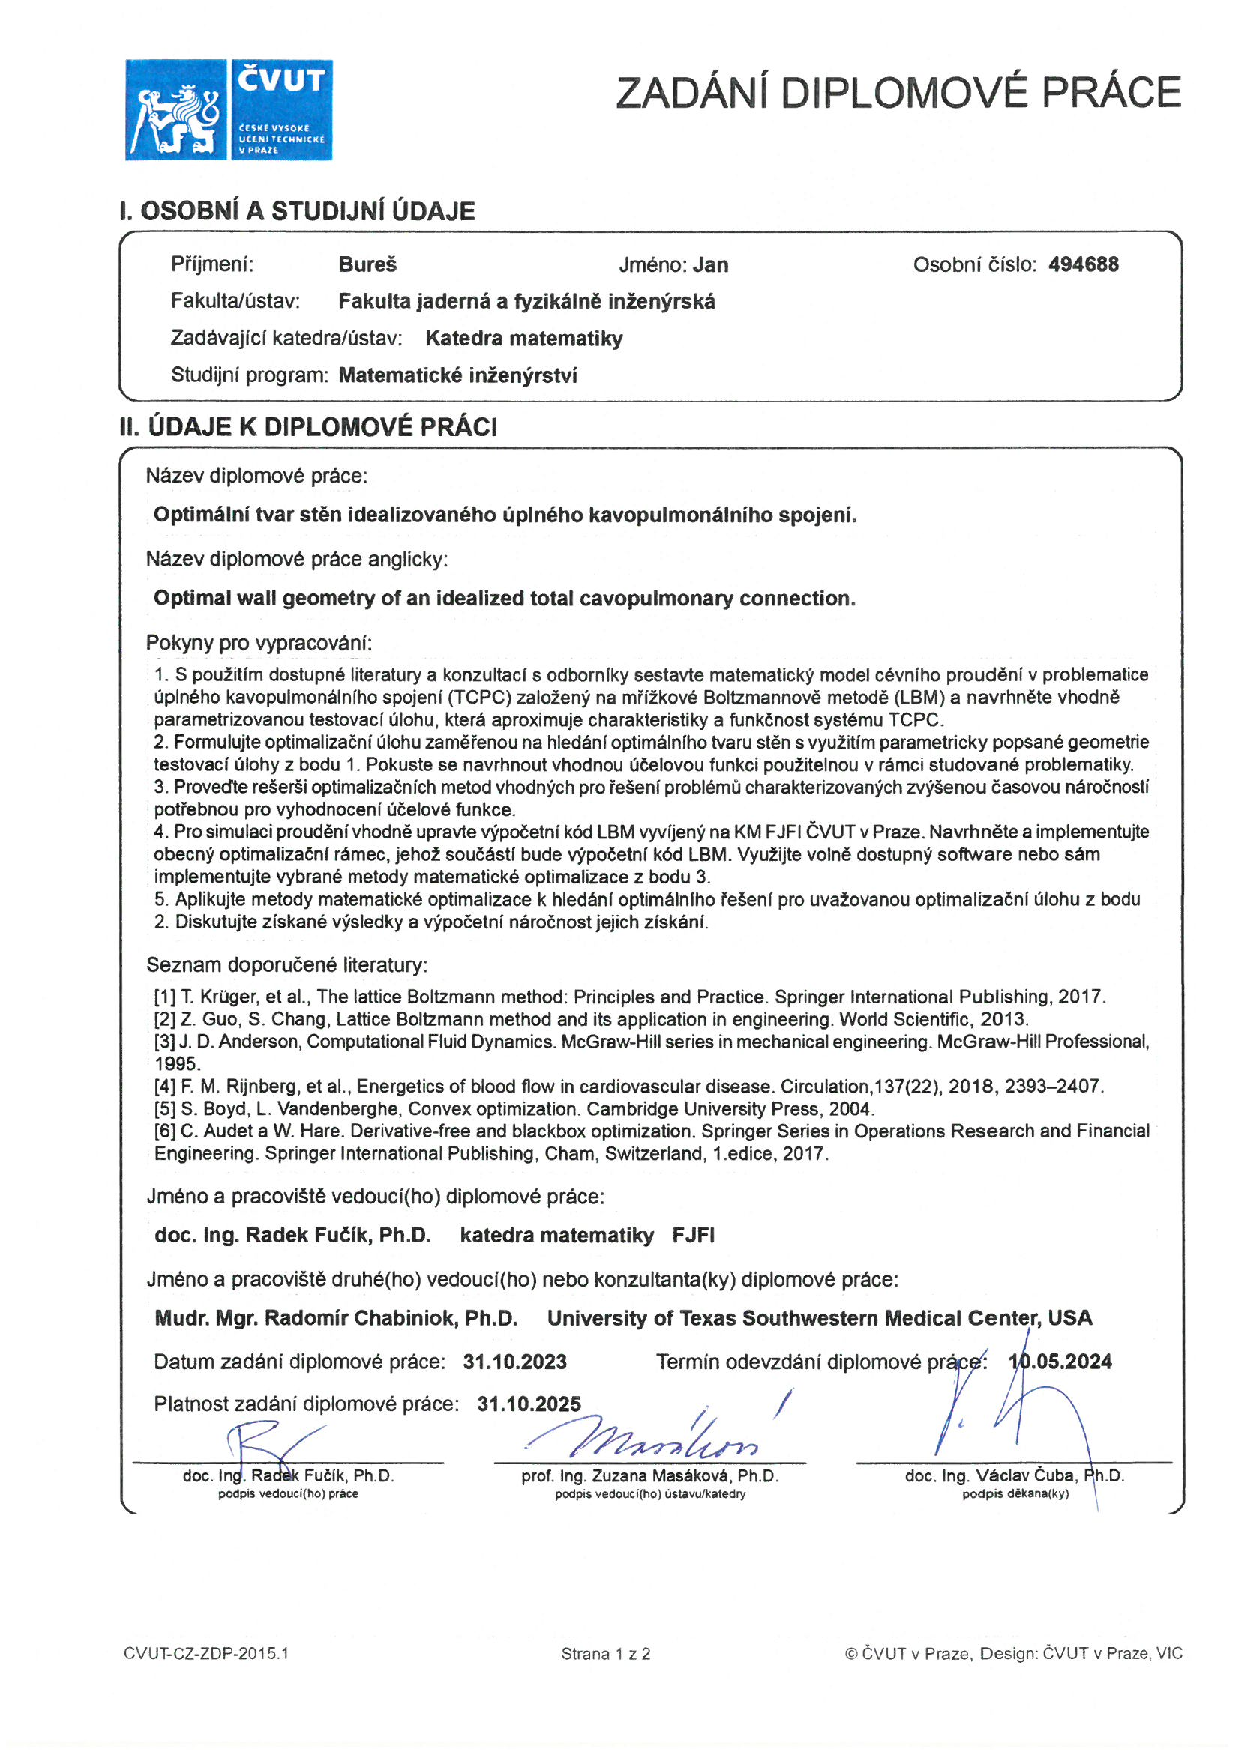
\includepdf[pages=-]{chapters/zadani_signed.pdf}

\newpage
\noindent \vspace*{0pt} % Ensure no vertical spacing before the text
\emph{\Large{}Acknowledgment:}{\Large\par}

\noindent I would like to express my gratitude to my supervisor, doc. Ing. Radek Fučík, Ph.D., whose guidance, expertise, and support were pivotal throughout this work. I am also deeply thankful to my consultant, MUDr. Mgr. Radomír Chabiniok, Ph.D., for his valuable insights on the medical aspects of this thesis.

\vspace*{\fill} % This stretches the space between the Acknowledgment and the Declaration

\noindent \emph{\Large{}Author’s declaration:}{\Large\par}

\noindent I declare that this thesis is entirely my own work and I have listed all the used sources in the bibliography.

\bigskip{}

\noindent Prague, January 2, 2025 \hfill{}Jan Bureš

\newpage{}
%~\newpage{}
\begin{onehalfspace}
\noindent \emph{Název práce:}
\noindent \textbf{Hledání optimálního tvaru stěn matematického modelu proudění krve v problematice úplného kavopulmonálního cévního napojení}
\end{onehalfspace}
\noindent \emph{Autor:} Bc. Jan Bureš\\[2pt]
\noindent \emph{Program:} Matematické inženýrství\\[2pt]
\noindent \emph{Druh práce:} Výzkumný úkol\\[2pt]
\noindent \emph{Vedoucí práce:} doc. Ing. Radek Fučík, Ph.D.,
Katedra matematiky a katedra softwarového inženýrství, FJFI ČVUT v Praze
Trojanova 13, 120 00 Praha\\[2pt]
\noindent \emph{Konzultant:} Ing. Pavel Eichler, Katedra softwarového inženýrství, FJFI ČVUT v Praze
Trojanova 13, 120 00 Praha 2\\[2pt]
\noindent \emph{Abstrakt:} Tato práce se zabývá optimalizací tvaru stěn v rámci modelování proudění nestlačitelné newtonovské tekutiny se zaměřením na modelování proudění krve v cévách. Je představen a implementován optimalizační rámec, který lze následně využít pro řešení optimalizačních úloh týkajících se proudění tekutin okolo rigidních překážek ve 2D. Pro numerické řešení matematického modelu je zvolena mřížková Boltzmannova metoda, která je stručně popsána.
Na hranici obtékaných těles jsou předepsány interpolační okrajové podmínky, které jsou popsány a dále použity. Díky interpolačním okrajovým podmínkám je zohledněn skutečný tvar hranice těles.
V teoretické části jsou pak dále popsány metody matematické optimalizace použité v této práci. Dále je popsán balík využitý k automatickému generování geometrií použitelných v numerických simulací, který byl implementován pro účely této práce. Praktická část demonstruje a analyzuje použití optimalizačního rámce na sérii vhodně navržených testovacích úloh. Na závěr jsou prezentovány výsledky optimalizační úlohy zjednodušeného modelu totálního kavopulmonálního spojení ve 2D, které jsou ve shodě s dostupnou literaturou. Použití optimalizačního rámce lze tedy považovat za úspěšné.

\bigskip{}

\noindent \emph{Klíčová slova:} matematická optimalizace, modelování proudění krve, mřížková Boltzmannova metoda, optimalizace tvarů, úplné kavopulmonární spojení
\vfill{}
~

%Interpolation boundary conditions are prescribed on the boundary of the enveloped bodies, which are described and used below. Due to the interpolation boundary conditions, the actual shape of the boundary of the bodies is taken into account.

\selectlanguage{american}%
\begin{onehalfspace}
\noindent \emph{Title:}
\noindent \textbf{Optimal shape design of walls of blood flow mathematical model focusing on the total cavopulmonary connection}
\end{onehalfspace}
\noindent \emph{Author:} Bc. Jan Bureš\\[2pt]
\noindent \emph{Abstract:} This thesis deals with the optimization of shape of walls and with flow modelling of incompressible Newtonian fluid with a focus on modelling of blood flow in blood vessels. An optimization framework is presented and implemented, which can then be used to solve optimization problems involving fluid flow around rigid objects in 2D. The lattice Boltzmann method is used as the numerical solver and is briefly described. The theoretical section then describes the mathematical optimization methods used in this work. Interpolation boundary conditions, which are described and later used, are prescribed on the boundary of the objects. Thanks to the interpolation boundary conditions, the actual shape of the boundary of the objects is taken into account. Furthermore, the package used to automatically generate geometries used in the numerical simulations, which was implemented for the purpose of this work, is described. The next part demonstrates and analyses the application of the optimization framework on a series of test problems. Finally, the results of the optimization problem of a simplified 2D total cavopulmonary connection model are presented, which are in agreement with the available literature. Thus, the application of the optimization framework can be considered successful.

\bigskip{}

\noindent \emph{Key words:} mathematical optimization, modeling of blood flow, lattice Boltzmann method, shape optimization, total cavopulmonary connection
\selectlanguage{czech}%
\newpage{}

%~\newpage{}

\pagestyle{plain}

\tableofcontents{}

\newpage{}

\chapter*{Introduction}

\addcontentsline{toc}{chapter}{Introduction}

This work deals with the mathematical modeling of fluid flow with a focus on finding the optimal shape of walls, particularly in the issue of total cavopulmonary connection. In many engineering fields such as the automotive or aerospace industries, incorporating optimization processes to find the optimal shape of the studied object is common practice. However, in the field of clinical medicine, for various reasons, the use of optimization techniques is still not so common. To obtain relevant results, it is necessary to model the complex blood flow inside often complicated geometries as accurately as possible using thoroughly tested methods. Validation of numerical simulation results against measured data is also often complicated, as performing experiments \textit{in vivo} (in a living organism) is naturally very difficult, sometimes even impossible.

Nevertheless, the process of shape optimization can find great potential especially in cardiac and vascular surgery \cite{Abraham2005, Weddell2015, Marsden2008}. Developing an optimization process usable in the medical environment would provide doctors with an \textit{in vitro} (outside a living organism) way to assess surgical procedures within patient-specific geometries. Designing and implanting objects such as stents or artificial valves would then be directly tailored to the patient's anatomy, which can lead to improved clinical outcomes, reduced risk of postoperative complications, and a general improvement in the patient's quality of life after the procedure \cite{Marsden2008}.

An example of a specific surgical procedure where the process of wall shape optimization can find its application is the so-called total cavopulmonary connection (\textit{TCPC}). TCPC is performed in children diagnosed with a so-called functionally single ventricle, i.e., in patients with a severe congenital heart defect, due to which their heart can effectively utilize only one functional ventricle, and in whom it is not possible to surgically ensure a functioning two-ventricle circulation \cite{Chaloup}. It is a surgery in which the superior vena cava (\textit{vena cava superior}, labeled \textit{d} in Fig.~\ref{fig:tcpc}) is surgically connected to the pulmonary artery. The inferior vena cava (\textit{vena cava inferior}, labeled \textit{b} in Fig.~\ref{fig:tcpc}) is also connected directly to the pulmonary artery (\textit{arteria pulmonalis}, labeled \textit{a} in Fig.~\ref{fig:tcpc}), usually using a so-called extracardiac conduit (labeled \textit{c} in Fig.~\ref{fig:tcpc}), or extracardiac channel, created from a vascular prosthesis \cite{Rubtsova, Delorme}.

\begin{figure}[h]
	\centering
	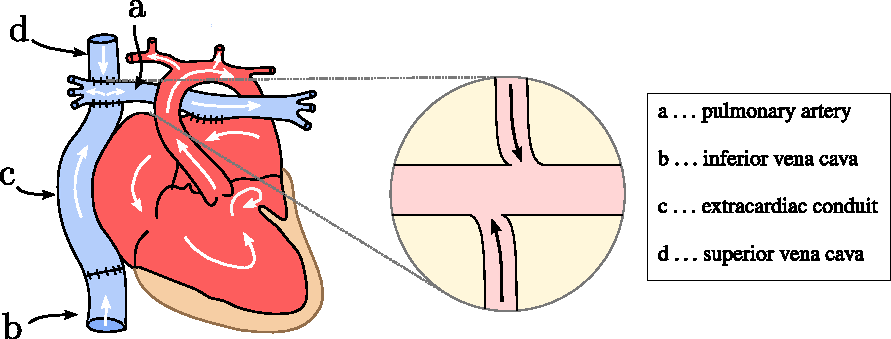
\includegraphics[width=0.97\textwidth]{figures/heart.pdf}
	\vspace{5mm}
	\caption{Diagram of the total cavopulmonary connection. The enlarged section shows the site of the extracardiac conduit connection.}
	\label{fig:tcpc}

\end{figure}

TCPC allows the creation of a functional blood circulation; however, the resulting circulatory system is specific and sensitive to several factors that undesirably contribute to energy loss in the system. This gradually leads to the overall failure of the system. These are mainly the influences of turbulent flow and collision of flows, which occur, for example, at the outlets of the superior and inferior vena cava into the pulmonary artery. The issue of optimal connection of the extracardiac conduit for the purpose of minimizing energy loss or minimizing tissue stress can be the subject of the optimization process \cite{Chaloup, vanBake, Wang}. There are a number of studies dealing with the design of the optimal shape of the conduit connection; however, they often rely only on the trial-and-error method and do not use optimization methods \cite{Rijnberg2018, Porfiryev2020, Tang2014}.

To create an optimization framework usable for cardiac surgery when simulating blood flow, it is necessary to use an efficient and reliable numerical method to compute the values of the objective function, which is subject to minimization. In this work, we use the lattice Boltzmann method (\textit{LBM}) for numerical computations. Note that for the LBM, a code developed at the Department of Mathematics of FNSPE CTU in Prague was used and modified according to the needs of this work. The main advantage of LBM is the possibility of massive parallelization on GPUs (graphics processing units), thanks to which computations take orders of magnitude less time than standard numerical methods used for modeling fluid flow \cite{PE, Kruger}. On the other hand, a significant disadvantage of LBM in terms of boundary geometry is that it uses a regular grid for spatial discretization. This presents a significant problem in the context of this work, as the boundaries of the bodies being modeled or the boundaries of vessels are discretized in a stair-step manner. Therefore, part of this work and the previous bachelor's thesis \cite{buresBP} is devoted to the study and implementation of interpolated boundary conditions, which allow the actual shape of the boundary of the modeled bodies to be taken into account within the discretization. Due to the use of these boundary conditions, even a small change in the shape of the geometry used in the numerical simulation leads to a change in the result obtained by the numerical simulation; therefore, within optimization, gradient optimization methods can be used, for example.

The structure of the work is as follows. The first chapter focuses on the mathematical model of fluid flow with an emphasis on modeling blood flow in vessels. The second chapter discusses the numerical method LBM in detail. In the third chapter, the tool developed for efficient parameterization and subsequent automatic geometry generation is further discussed. The fourth chapter contains the theory of mathematical optimization and the optimization methods used in this work; moreover, the proposed optimization framework is presented in this chapter. The last chapter presents the results of the numerical simulations performed. First, the functionality of the used optimization framework is tested on a series of designed test problems with one optimization parameter. Then, optimization is tested on more complex problems with multiple optimization parameters, and among other things, the influence of the optimization method used and the choice of the initial solution estimate is examined. One of the more complex problems includes a simplified 2D model of a vascular junction arising in total cavopulmonary connection.




\chapter{Mathematical model}


\chapter{Lattice Boltzmann method}\label{lbm}

We can consider a fluid as a continuum and use a macroscopic description, meaning we view the fluid as a whole and utilize macroscopic quantities such as density, flow velocity, or pressure for the state description, with the governing equations being \eqref{NS}. On the other hand, we can describe the dynamics of each particle in a given volume and thus use a microscopic description. Describing the dynamics of a particle at a microscopic scale is not difficult, but a significant drawback of this approach is its evident computational complexity, which is directly proportional to the number of particles being studied.

A middle ground between the above-mentioned descriptions is the mesoscopic description \cite{PE}, which is based on kinetic theory. The fluid is described using one-particle probability distribution functions of density \( f(\vec{x},\vec{\xi}, t) \) \si{[kg.s^3.m^{-6}]}, which describe the system in the space of coordinates \( \vec{x} \), microscopic velocities \( \vec{\xi} \), and time \( t \). The distribution functions \( f \) give the density of particles occurring in the vicinity of \( \vec{x} \) at time \( t \) with a microscopic velocity \( \vec{\xi} \).

The one-particle distribution functions in the vicinity of \( \vec{x} \) satisfy the Boltzmann transport equation \cite{Kruger}
\begin{equation}\label{eq:BTR}
	\frac{\partial f}{\partial t} + \sum_{i = 1}^{3} \xi _{i} \frac{\partial f}{\partial x_{i}} + \sum_{i = 1}^{3} g_{i} \frac{\partial f}{\partial \xi _{i}} = \mathcal{C}(f), 
\end{equation}
where \( \vec{g} \) \si{[m.s^{-2}]} is the acceleration vector of external forces, and \( \mathcal{C}(f)\) \si{[kg.s^2.m^{-6}]} is the collision operator.

Using the distribution functions \( f \), certain macroscopic quantities can be expressed as statistical moments \cite{Kruger}, such as

\begin{subequations}\label{eq:macroscopic basic}
	\begin{alignat}{1}
		\rho(\vec{x}, t) & =\int\displaylimits_{\mathbb{R}^3} f(\vec{x}, \vec{\xi}, t) \mathrm{~d} \vec{\xi} \label{subeq:rho}, \\
		\rho(\vec{x}, t) \vec{u}(\vec{x}, t) & =\int\displaylimits_{\mathbb{R}^3} f(\vec{x}, \vec{\xi}, t) \, \vec{\xi} \mathrm{~d} \vec{\xi} \label{subeq:momentum}.
	\end{alignat}
\end{subequations}


The lattice Boltzmann method (LBM) is a numerical method based on the mesoscopic description of fluids. The numerical scheme of LBM can be derived by discretizing \eqref{eq:BTR}. In LBM, the spatial discretization is performed using a discrete equidistant lattice, and the discretization of velocity space is carried out using a finite set of microscopic velocities. We introduce velocity models denoted as D$d$Q$q$, where $ d$ and $q$ represent the dimension of the considered space and the number of different directions in which movement from each lattice node is possible, respectively.

In this thesis, we consider the D3Q27 velocity model, which is schematically shown in Figure~\ref{fig:d3q27}.

\begin{figure}[h]
	\centering
	\vspace{4mm}
	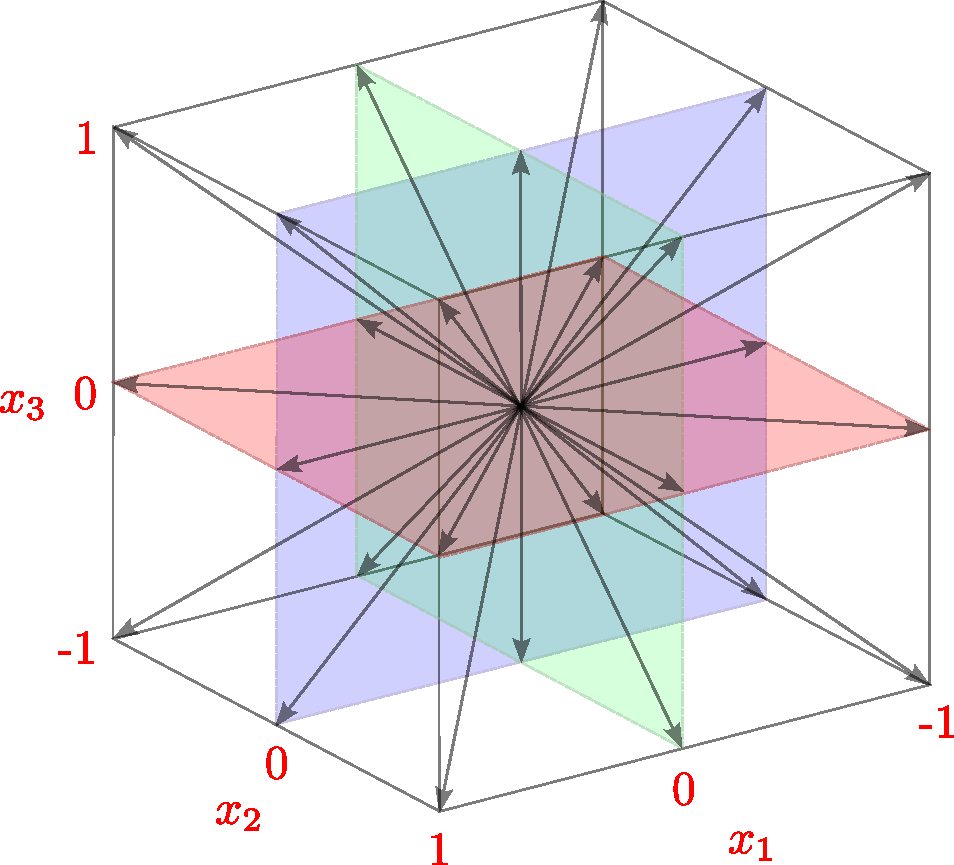
\includegraphics[width=.6\textwidth]{figures/d3q27.pdf}
	\caption{Geometric representation of the D3Q27 velocity model.}
	\label{fig:d3q27}
\end{figure}

The velocity space of the microscopic particle velocity is discretized by a finite set of microscopic velocities, which, in the case of the D3Q27 model, is defined as

\begin{equation}\label{eq:velocities}
	\begin{gathered}
		\left(\boldsymbol{\xi}_k\right)_{k=1}^{27}=\left(\left(\begin{array}{l}
			0 \\
			0 \\
			0
		\end{array}\right),\left(\begin{array}{l}
			1 \\
			0 \\
			0
		\end{array}\right),\left(\begin{array}{l}
			0 \\
			1 \\
			0
		\end{array}\right),\left(\begin{array}{l}
			0 \\
			0 \\
			1
		\end{array}\right),\left(\begin{array}{c}
			-1 \\
			0 \\
			0
		\end{array}\right),\left(\begin{array}{c}
			0 \\
			-1 \\
			0
		\end{array}\right),\left(\begin{array}{c}
			0 \\
			0 \\
			-1
		\end{array}\right)\right., \\
		\left.\left(\begin{array}{l}
			0 \\
			1 \\
			1
		\end{array}\right),\left(\begin{array}{c}
			0 \\
			1 \\
			-1
		\end{array}\right),\left(\begin{array}{c}
			0 \\
			-1 \\
			1
		\end{array}\right),\left(\begin{array}{c}
			0 \\
			-1 \\
			-1
		\end{array}\right),\left(\begin{array}{l}
			1 \\
			1 \\
			0
		\end{array}\right),\left(\begin{array}{c}
			1 \\
			-1 \\
			0
		\end{array}\right),\left(\begin{array}{c}
			-1 \\
			1 \\
			0
		\end{array}\right),\left(\begin{array}{l}
			-1 \\
			-1 \\
			0
		\end{array}\right),\left(\begin{array}{l}
			1 \\
			0 \\
			1
		\end{array}\right),\left(\begin{array}{l}
			1 \\
			0 \\
			-1
		\end{array}\right)\right., \\
		\left.\left(\begin{array}{c}
			-1 \\
			0 \\
			1
		\end{array}\right),\left(\begin{array}{c}
			-1 \\
			0 \\
			-1
		\end{array}\right),\left(\begin{array}{l}
			1 \\
			1 \\
			1
		\end{array}\right),\left(\begin{array}{c}
			1 \\
			1 \\
			-1
		\end{array}\right),\left(\begin{array}{c}
			1 \\
			-1 \\
			1
		\end{array}\right),\left(\begin{array}{c}
			1 \\
			-1 \\
			-1
		\end{array}\right),\left(\begin{array}{c}
			-1 \\
			1 \\
			1
		\end{array}\right),\left(\begin{array}{c}
			-1 \\
			1 \\
			-1
		\end{array}\right),\left(\begin{array}{c}
			-1 \\
			-1 \\
			1
		\end{array}\right),\left(\begin{array}{l}
			-1 \\
			-1 \\
			-1
		\end{array}\right)\right).
	\end{gathered}
\end{equation}

\section{Non-dimensionalization and discretization}
The computational domain \( (0 ; L_1) \times(0 ; L_2) \times(0 ; L_3)\), where \( L_i\) \si{[m]}, $i=1,2,3$, represent the dimensions of the domain, is discretized using an equidistant grid with a spatial step size \( \Delta l \) \si{[m]}. The time interval is discretized uniformly using a time step size \( \Delta t \)~\si{[s]}.

In LBM, it is common to work with non-dimensional quantities instead of physical ones, as discussed in \cite{Kruger}. This section introduces the conversion relationships for transitioning to a non-dimensional system, defines the lattice used for domain discretization, and describes the discretized Boltzmann transport equation.

\subsection{Non-dimensional units}
The transition between unit systems can be performed using the law of similarity for fluid dynamics, which ensures that the values of relevant non-dimensional quantities remain constant \cite{Kruger}. One such non-dimensional quantity that can be used during the transition is, for example, the Reynolds number \eqref{Re}. It should be emphasized that the physical principles remain valid regardless of the choice of the unit system. 

In the following conversion relations, all quantities in lattice units are marked with the superscript \( L \). It can be shown \cite{Kruger} that the following holds:
\begin{eqnarray}
	l^{L}_0 &=& \dfrac{l_{0}}{\Delta l},\\[5pt]
	t^{L}_0 &=& \dfrac{t_{0}}{\Delta t},\\[5pt]
	\nu^L &=& \nu \dfrac{\Delta t}{\Delta l^{2}},\\[5pt]
	u^{L}_{i} &=& \dfrac{\Delta t}{\Delta l} u_{i}, \ i \in \{1, 2, 3\}.
\end{eqnarray}
The characteristic length, time, and velocity values are chosen based on the given physical problem. The computational domain's largest dimension or the size of an obstacle within the flow is typically chosen as \( l_{0} \). Detailed derivations of these relations can be found in \cite{Kruger}. From the relationship for kinematic viscosity, it can be seen that for a given spatial step \( \Delta l \), the time step \( \Delta t \) is linked to the value of \( \nu^L \).

For simplicity, in this work, we will assume that the spatial step \( \Delta l ^L \) and the time step \( \Delta t ^L \) in lattice units are \( \Delta l ^L  =  \Delta t ^L = 1 \). In the remainder of this chapter, we use lattice units exclusively and for brevity we omit the superscript \( L \), though all quantities will be non-dimensional.
\subsection{Computational Domain and Discrete Grid}
From this point forward, we assume that all quantities are expressed in lattice units, meaning $ \Delta l $ and $ \Delta t $ now represent non-dimensional spatial and time steps, respectively. We consider a cuboidal computational domain $ \Omega \subset \mathbb{R}^3 $, see section \ref{pred}. This domain in LBM is discretized using an equidistant grid

\begin{subequations}\label{eq:domain}
	\begin{eqnarray}
		&\hat{\Omega} = \left\{ \vec{x}_{i,j,k} = (i \Delta l,\,j \Delta l, \,k \Delta l)^T \ \middle| \ i \in \{1, \dots, N_{1} - 1\}, j \in \{1, \dots, N_{2} - 1 \}, k \in \{1, \dots, N_{3} - 1 \} \right\},\\[4pt]
		&\overline{\hat{\Omega}} = \left\{ \vec{x}_{i,j} = (i \Delta l,\,j \Delta l)^T \ \middle| \ i \in \{0, \dots, N_{1} \}, j \in \{0, \dots, N_{2} \}, k \in \{0, \dots, N_{3} \} \right\},
	\end{eqnarray}
\end{subequations}
where $ N_{i} $ [-] denotes the number of grid points in the $ x_i $ direction, $ i = 1, 2, 3 $.

The boundary of the domain $ \Omega $ will be denoted by $ \partial \Omega $ and understood as the closure of the disjoint union of the individual parts 
\begin{equation}\label{eq:border decomposition}
	\partial \Omega = \overline{\partial \Omega_{\mathrm{W}} \cup \partial \Omega_{\mathrm{E}} \cup \partial \Omega_{\mathrm{N}} \cup \partial \Omega_{\mathrm{S}} \cup \partial \Omega_{\mathrm{F}} \cup \partial \Omega_{\mathrm{B}}},
\end{equation}
where the meanings of $\partial \Omega_{\mathrm{W}} , \partial \Omega_{\mathrm{E}} , \partial \Omega_{\mathrm{N}}, \partial \Omega_{\mathrm{S}}, \partial \Omega_{\mathrm{F}}$, $  \partial \Omega_{\mathrm{B}} $ are illustrated in Figure \ref{fig:domain}. We will further consider the discretization of the boundary of the computational domain as
\begin{equation}\label{eq:border}
	\partial\hat{\Omega} = \overline{\hat{\Omega}} \, \backslash \, \hat{\Omega},
\end{equation}
with the corresponding parts of the discrete boundary denoted as $ \partial \hat{\Omega}_{\mathrm{W}} , \partial \hat{\Omega}_{\mathrm{E}} , \partial \hat{\Omega}_{\mathrm{N}}, \partial \hat{\Omega}_{\mathrm{S}}, \partial \hat{\Omega}_{\mathrm{F}}$,  and $ \partial \hat{\Omega}_{\mathrm{B}} $.
\begin{figure}[H]
	\centering
	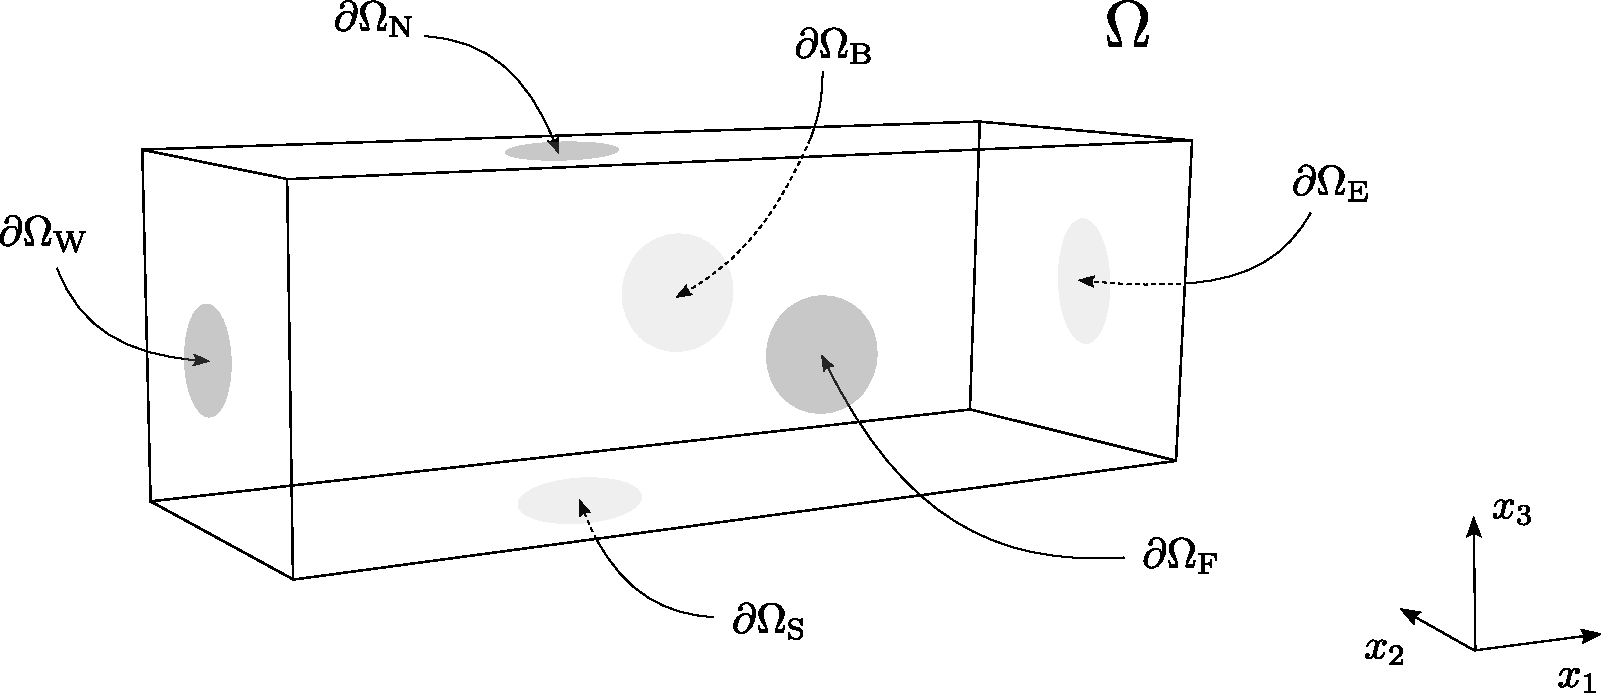
\includegraphics[width=0.99\textwidth]{figures/omega.pdf}
	\caption{Schematic representation of the computational domain $ \Omega $ and its boundary $ \partial \Omega $.}  
	\label{fig:domain}
	\vspace{1.8mm}
\end{figure}

The time interval over which the problem will be investigated will be denoted by $ \mathcal{I} $ , where ${\mathcal{I} = \langle 0, T \rangle}$, and $ T > 0 $. The interval $ \mathcal{I} $ is discretized as
\begin{equation}\label{eq:timediscrete}
	\hat{\mathcal{I}} = \left\{ t_{i} = i \frac{T}{N_t} \ \middle| \ i \in \left\{0, \dots, N_{t} \right\} \right\},
\end{equation}
where $ N_t $ represents the number of discrete time steps for the discretization of the interval $ \mathcal{I} $.

\subsection{Discrete Boltzmann transport equation}
When using the D3Q27 model, we work with a set of distribution functions
\begin{equation}\label{eq:ddfs}
	\left\{ f_k (\vec{x}, t) \ \middle| \ k = 1, \dots, 27 \right\}, \ \forall \vec{x} \in \hat{\Omega}, \ \forall t \in \hat{\mathcal{I}},
\end{equation}
where the indices correspond to the directions of microscopic velocities from \eqref{eq:velocities}.

It can be shown that by discretizing the equation \eqref{eq:BTR}, we obtain the form
\begin{equation}\label{eq:BTRdiscrete}
	f_{k}\left(\vec{x}+\Delta t \vec{\xi}_{k}, t+\Delta t \right) =
	f_{k}(\vec{x}, t) + \mathcal{C}_{k}(\vec{x}, t) + \mathcal{S}_{k}(\vec{x}, t), \hspace{2.5mm} k \in \{1, \dots, 27 \}, \ \forall \vec{x} \in \hat{\Omega}, \ \forall t \in \hat{\mathcal{I}},
\end{equation}
where $ \mathcal{C}_{k} $ represents the discrete collision operator and $ \mathcal{S}_{k} $ is the discrete forcing term. Details of the derivation of the discrete form of the Boltzmann transport equation can be found in \cite{Kruger}.

The discrete collision operator $\mathcal{C}_{k}$ in equation \eqref{eq:BTRdiscrete} defines the specific variant of LBM. Several choices for $\mathcal{C}_{k}$ exist, each corresponding to different LBM formulations. These include, for instance, the single relaxation time (SRT-LBM) \cite{GeierCuLBM}, multiple relaxation time (MRT-LBM) \cite{MRT}, central moment (CLBM) \cite{GeierCLBM}, entropic (ELBM) \cite{ELBM}, and cumulant-based (CuLBM) \cite{GeierCuLBM} approaches. In this work, we use the cumulant collision operator, as detailed in \cite{GeierCuLBM}.


We can further introduce the post-collision distribution functions $ f^{*}_{k} $ as
\begin{equation}\label{eq:fstar}
	f^{*}_{k}(\vec{x}, t) = f_{k}(\vec{x}, t) + \mathcal{C}_{k}(\vec{x}, t) + \mathcal{S}_{k}(\vec{x}, t), \hspace{2.5mm} k \in \{1, \dots, 27 \}, \ \forall \vec{x} \in \hat{\Omega}, \ \forall t \in \hat{\mathcal{I}}.
\end{equation}
Using $ f^{*}_{k} $, we can express \eqref{eq:BTRdiscrete} in the form
\begin{equation}\label{eq:collision}
	f_{k}\left(\vec{x}+\Delta t \vec{\xi}_{k}, t+\Delta t\right) = f^{*}_{k}(\vec{x}, t), \hspace{2.5mm} k \in \{1, \dots, 27 \}, \ \forall \vec{x} \in \hat{\Omega}, \ \forall t \in \hat{\mathcal{I}},
\end{equation}
which can be interpreted as an explicit prescription for calculating the distribution functions.
\subsection{Macroscopic Quantities}\label{macro}
Finally, we present the relations for calculating some of the macroscopic quantities. Some of these relations can be derived through the process of discretization from the general relations \eqref{eq:macroscopic basic} \cite{Kruger}. The relations for calculating density, momentum, and pressure are as follows:

\begin{subequations}\label{macroeq}
	\begin{eqnarray}
		\label{rho}
		\rho &=& \sum_{k=1}^{27} f_{k},\\[3pt]
		\rho \vec{u} &=& \sum_{k=1}^{27} f_{k} \vec{\xi_{k}} + \rho \dfrac{\Delta t}{2} \vec{g},\\[3pt]
		p &=& p_0 + c_{s}^{2} (\rho - \rho_0),
	\end{eqnarray}
\end{subequations}
where $ p_0 $ \si{[-]} is the non-dimensional reference value of pressure, $ c_s $ \si{[-]} is the non-dimensional (lattice) speed of sound, and $ \rho_0 $ is the non-dimensional reference value of density. For $ c_s $ in the D3Q27 model, $ c_s = \frac{1}{\sqrt{3}} $. Furthermore, we consider $ \rho_0 = 1 $. A detailed description of the calculation of macroscopic quantities is provided in \cite{Kruger}.
\section{LBM algorithm}\label{algoritmus LBM}
The LBM algorithm can be summarized in several steps:
\begin{enumerate}
	\item \textbf{Initialization} of initial conditions on the grid, discussed in section \ref{pocatecni a okrajove podminky}.
	\item \textbf{Cycle} ending with the fulfillment of a user-specified termination condition.
	\begin{enumerate}
		\item \textbf{Streaming} of post-collision distribution functions \( f^{*}_{k} \) in the respective directions \( \vec{\xi_{k}} \).
		\item \textbf{Calculation of macroscopic quantities} using the relations \eqref{macroeq}.
		\item \textbf{Collision}, where the post-collision state of the distribution function is calculated using \eqref{eq:collision}, and \textbf{application of boundary conditions}, discussed in section \ref{pocatecni a okrajove podminky}.
	\end{enumerate}
	\item \textbf{End of the algorithm.}
\end{enumerate}
A flowchart of the LBM algorithm is shown in Figure \ref{fig:algo}.
\begin{figure}[h]
	\centering
	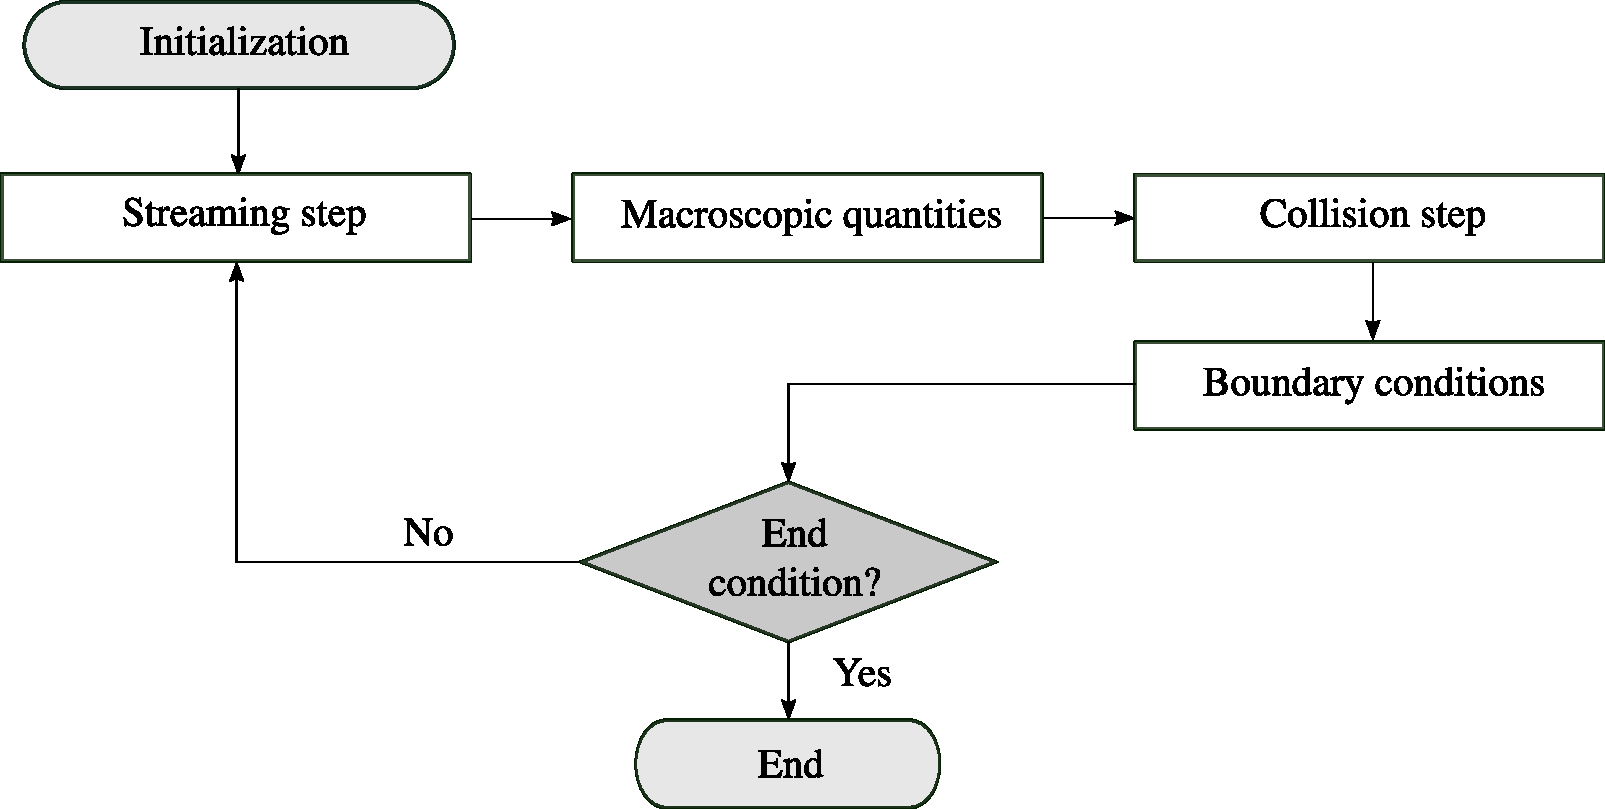
\includegraphics[width=0.78\textwidth]{figures/algo-bw.pdf}
	\caption{Flowchart of the LBM algorithm.}
	\label{fig:algo}
\end{figure}
\input{chapters/lbm/collision.tex}
\section{Initial and boundary conditions}\label{pocatecni a okrajove podminky}

The choice of initial and boundary conditions is an integral part of the lattice Boltzmann method to ensure consistency the mesoscopic description. Therefore, the chosen initial and boundary conditions are described in more detail in this section.

\subsection{Initial condition}\label{pocatecni podminka}
Let us now consider the domain defined by relations \eqref{eq:domain}. In this work, the equilibrium distribution function \( f^{\mathrm{eq}} \) is used to set the initial condition. The equilibrium distribution function is given by
\begin{equation}\label{eq:feq}
	f^{\mathrm{eq}}_{k} = \rho w_{k} \, \left(1 + \frac{\vec{\xi_{k}} \cdot \vec{u}}{c^{2}_{s}} + \frac{(\vec{\xi_{k}} \cdot \vec{u})^2}{2c^{4}_{s}} - \frac{\vec{u} \cdot \vec{u}}{2c^{2}_{s}} \right)\, , \hspace{2mm} k \in \{1,\dots,27\},
\end{equation}
where \( w_{k} \) are the weights specific to the chosen velocity model. For the D3Q27 model, these weights are defined as \cite{Kruger}
\begin{equation}
	w_k= \begin{cases}\frac{8}{27}, & k=1, \\ \frac{2}{27}, & k = 2,3, \ldots, 7, \\ \frac{1}{54}, & k = 8,9, \ldots, 19, \\ \frac{1}{216}, & k = 20,21, \ldots, 27.\end{cases}
\end{equation}
The initial density \( \rho \) and the velocity \( \vec{u} \), are denoted as \( \rho _{\mathrm{ini}} \) and \( \vec{u} _{\mathrm{ini}} \), respectively. At each lattice node \( \vec{x} \in \hat{\Omega} \) at time \( t=0 \), the distribution functions are initialized as
\begin{equation}\label{eq:initial condition}
	f^{}_{k} (\vec{x}, 0) = f^{\mathrm{eq}}_{k} (\rho _{\mathrm{ini}} (\vec{x}), \vec{u} _{\mathrm{ini}} (\vec{x})), \hspace{3mm} k \in \{1, \dots 27\}.
\end{equation}

This approach assumes that the non-equilibrium component of the distribution functions, defined as \( f^{\mathrm{neq}}_{k} = f_{k} - f^{\mathrm{eq}}_{k} \), can be neglected, and the distribution functions can be approximated by their equilibrium part. A significant advantage of this choice of initial condition approximation is its easy implementation. While more advanced initialization methods exist  \cite{PE}, the equilibrium-based approach is used in this work.

\subsection{Boundary conditions}


\subsubsection*{Bounce-back boundary condition}\label{bounce-back}
The first boundary condition discussed is the bounce-back boundary condition, specifically its \textit{fullway} variant \cite{Kruger}. The bounce-back boundary condition is typically used for modeling the interface between a fluid and a solid. Its advantage is that it satisfies the no-slip condition at the fluid-solid interface while remaining straightforward to implement. The principle of the bounce-back boundary condition is that at the interface, the distribution functions corresponding to particles with microscopic velocity \( \vec{\xi_{k}} \) are reflected back into the directions from which they arrived at the node, with velocity \( \vec{\xi_{\bar{k}}} = -\vec{\xi_{k}} \).

When using this boundary condition, the fluid-solid interface is located halfway between the fluid and solid nodes. For curved boundaries that are not parallel to the grid, the bounce-back method leads to a "staircase" shape of the boundary, which can limit the accuracy of the simulation.

In this approach, particles are reflected over two time steps. During this time, the particles reach the solid nodes, where their direction is reversed and they are streamed back, as schematically shown in Figure \ref{fig:fbb}.

\begin{figure}[h]
%	\vspace{-.5cm}
	\centering

	\begin{subfigure}{0.48\textwidth}
		\centering
		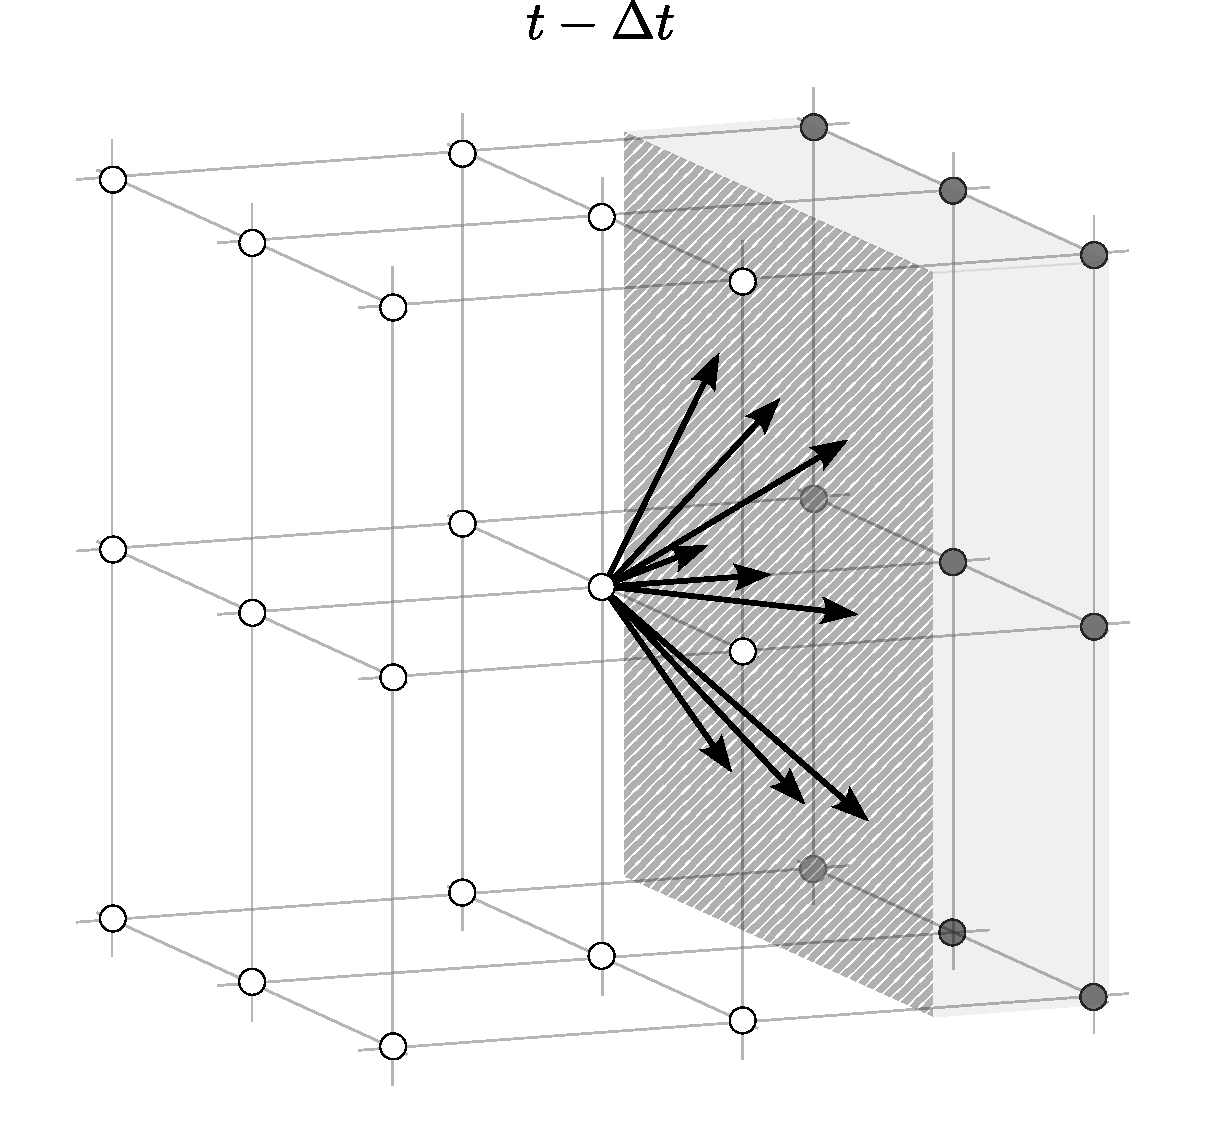
\includegraphics[width=0.9\textwidth, trim={0mm 0mm 0mm 0mm}]{figures/fwbba.pdf}
		\caption{Step before the streaming at time $t - \Delta t$.}
		\label{fig:bba}
	\end{subfigure}
	\begin{subfigure}{0.48\textwidth}
		\centering
		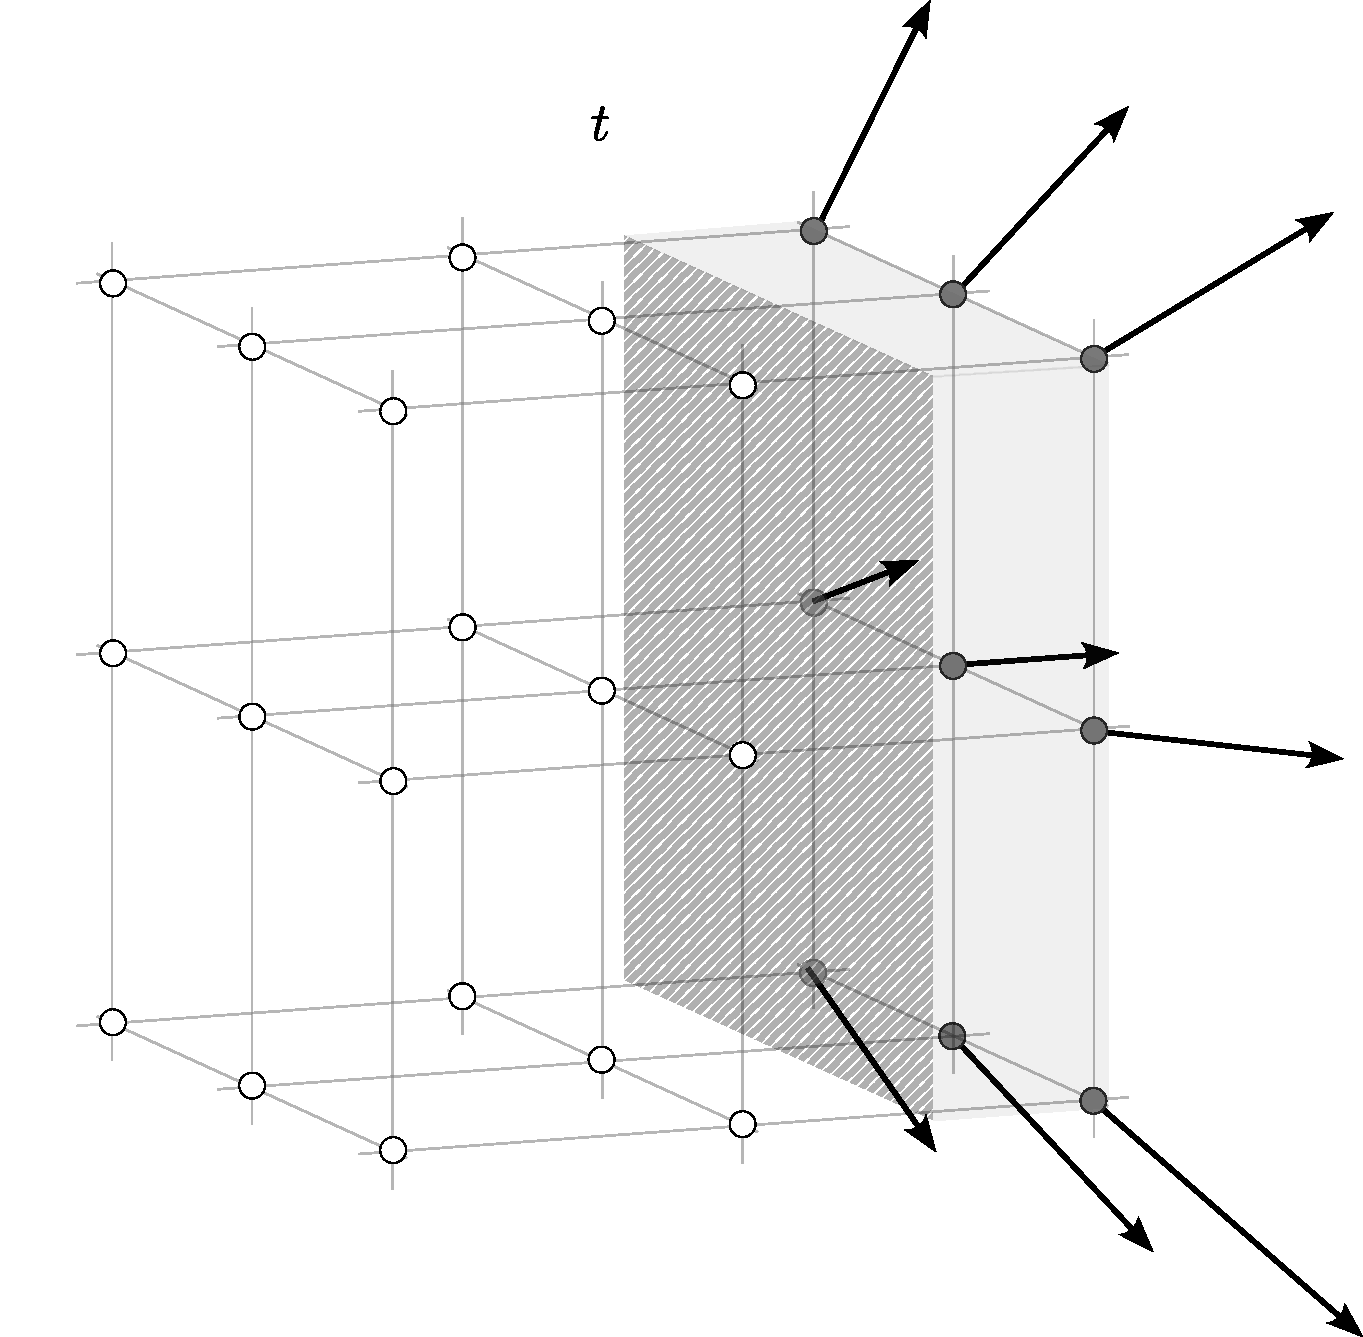
\includegraphics[width=0.9\textwidth, trim={0mm 0mm 0mm 0mm}]{figures/fwbbb.pdf}
		\caption{Step after streaming at time $t$.}
		\label{fig:bbb}
	\end{subfigure}
	\par\bigskip
	\par\bigskip
	\begin{subfigure}{0.48\textwidth}
		\centering
		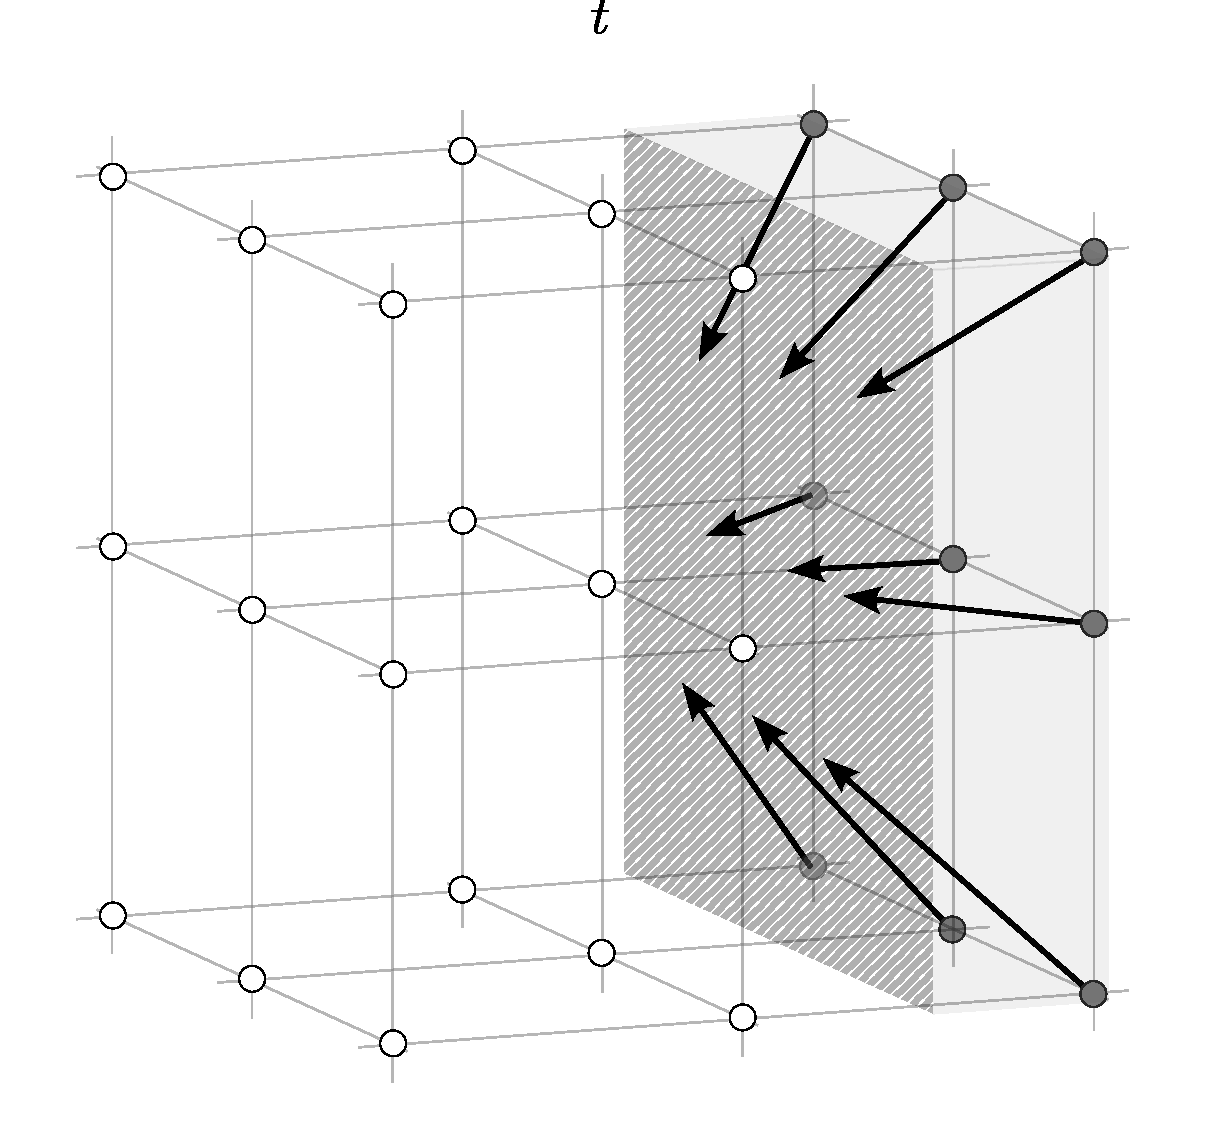
\includegraphics[width=0.9\textwidth, trim={0mm 0mm 0mm 0mm}]{figures/fwbbc.pdf}
		\caption{The distribution functions are reversed.}
		\label{fig:bbc}
	\end{subfigure}
	\begin{subfigure}{0.48\textwidth}
		\centering
		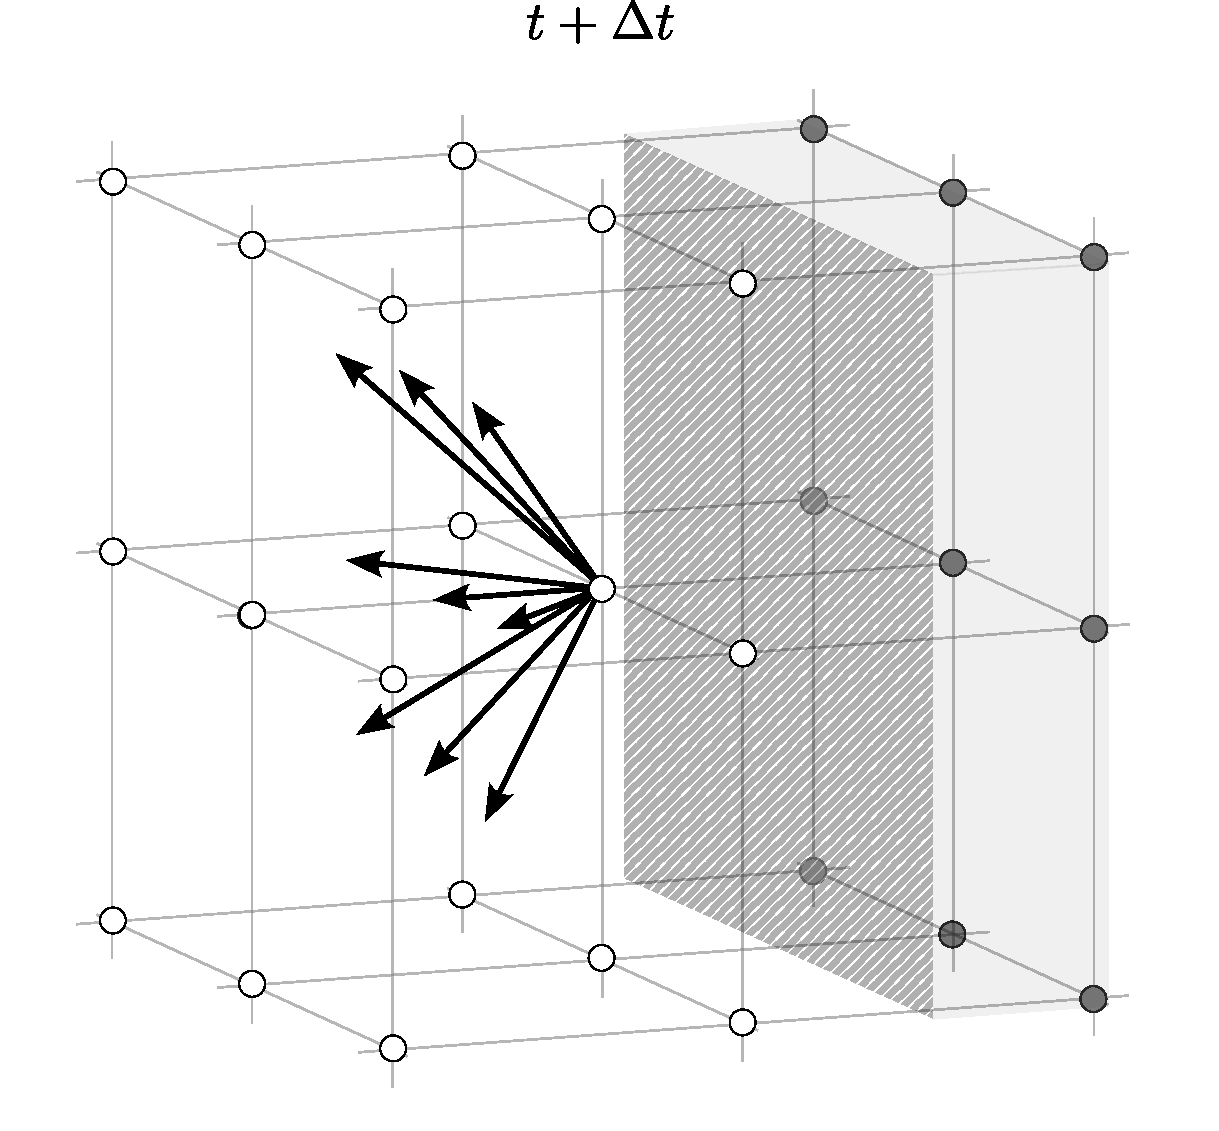
\includegraphics[width=0.9\textwidth, trim={0mm 0mm 0mm 0mm}]{figures/fwbbd.pdf}
		\caption{Step after the streaming at time $t + \Delta t$.}
		\label{fig:bbd}
	\end{subfigure}
	\vspace{5mm}
	\caption{Schematic representation of the fullway bounce-back boundary condition for the D3Q27 velocity model. White points represent fluid nodes, and gray points represent wall nodes. The wall is represented by a gray plane.}
	\label{fig:fbb}
\end{figure}

An alternative to the fullway method is the \textit{halfway} variant of the bounce-back boundary condition, which completes the reflection process within a single time step. Details can be found in \cite{Kruger}. In this work, however, we limit ourselves to the fullway variant.

%\subsubsection{Equilibrium boundary condition}\label{equilibrium bc}
%One option for approximating unknown distribution function values at the boundary nodes is to use the equilibrium distribution function, defined as \cite{PE}
%\begin{equation}
%	f_i(\vec{x}, t)=f_{i}^{\text{(eq)}}(\rho(\vec{x}, t), \vec{u}(\vec{x}, t)), \hspace{2mm}  \forall k \in \{1,\dots,27\}, \forall t \in \hat{\mathcal{I}}.
%\end{equation}
%The advantage of this approximation is its simple implementation, while the disadvantage is the neglect of the non-equilibrium part of the distribution function \cite{PE}.

%\subsubsection{Symmetric boundary condition}\label{symmetric bc}
%The symmetric boundary condition assumes that the domain is symmetric relative to a given mirror plane. This boundary condition can be understood as a bounce-back-like method. The distribution functions leave the boundary node at time $t$, meet the symmetry surface at time $t + \frac{\Delta t}{2}$, where they are mirrored, and return to the fluid nodes at time $t + \Delta t$. The components of the mirrored velocity depend on the normal vector of the symmetry plane, the tangential components of the velocity remain unchanged. The symmetric boundary condition is illustrated in Figure~\ref{fig:symmetric bc}.
%\vspace{2mm}
%\begin{figure}[H]
%	\centering
%	\begin{subfigure}{0.47\textwidth}
%		\centering
%		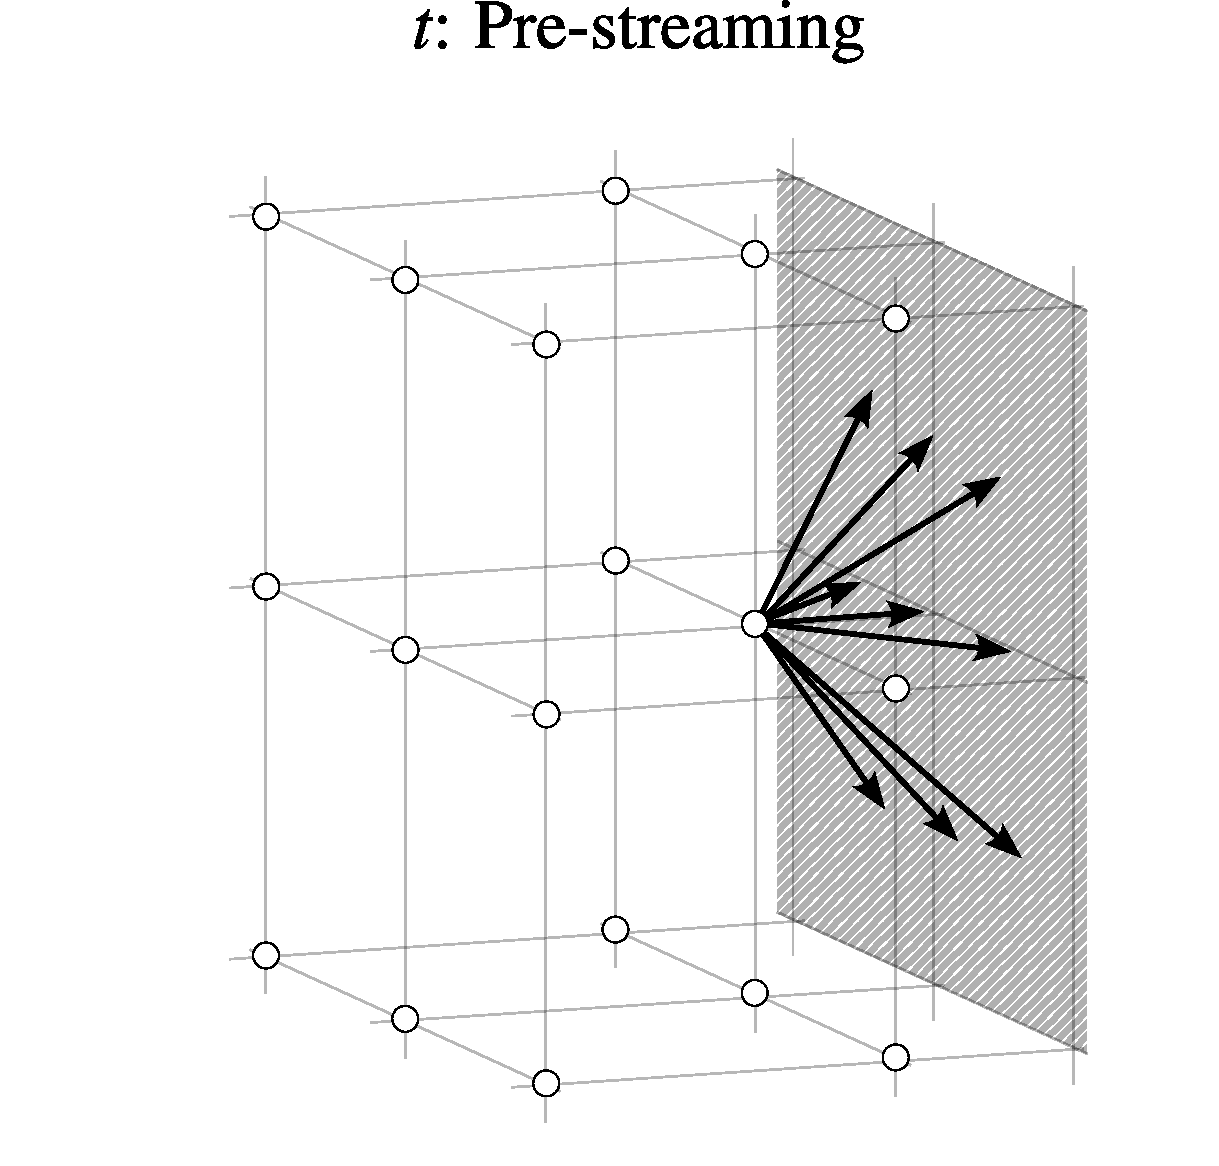
\includegraphics[width=0.99\textwidth, trim={0mm 0mm 0mm 0mm}]{figures/symmetric-a.pdf}
%		\caption{The distribution functions leave the boundary node at time $t$.}
%		\label{fig:sym a}
%	\end{subfigure}\hfill% 
%	\begin{subfigure}{0.47\textwidth}
%			\centering
%			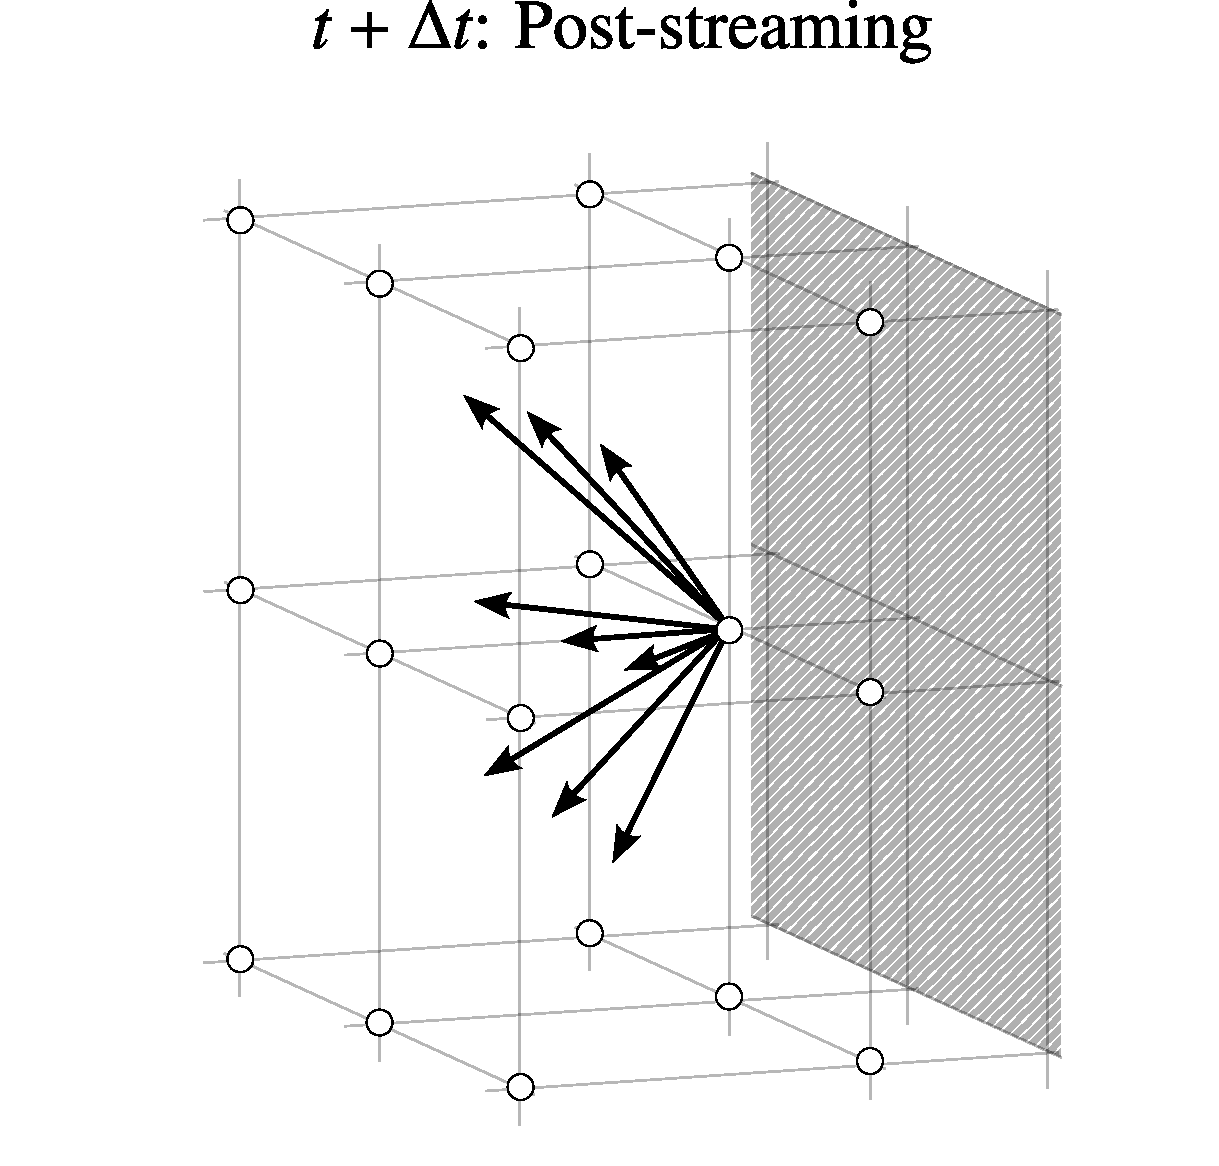
\includegraphics[width=0.99\textwidth, trim={0mm 0mm 0mm 0mm}]{figures/symmetric-b.pdf}
%			\caption{The mirrored distribution functions return to fluid nodes at time $t + \Delta t$.}
%			\label{fig:sym b}
%	\end{subfigure}
%	\vspace{2mm}
%	\caption{Illustration of the symmetric boundary condition for the symmetry plane with the normal vector \( (-1, 0, 0) \) using the D3Q27 velocity model. White points represent fluid nodes, and gray plane resents the symmetry plane.}
%	\label{fig:symmetric bc}
%
%\end{figure}

\subsubsection*{Free outflow boundary condition}\label{symmetric bc}
When using the free outflow boundary condition at the outlets, each distribution function for directions pointing out of the domain is set equal to the value it had at the adjacent node inside the computational domain in the previous timestep. While this boundary condition is numerically stable, its usage can cause unphysical behavior of pressure and velocity field near the outflow boundary. Details on the free outflow boundary condition can be found in \cite{PE}.
\section{Notes on the implementation}\label{poznamky k implementaci LBM}
As mentioned in the introduction, the numerical solution using LBM was based on a code developed at the Department of Mathematics of FNSPE, CTU in Prague, which is used to solve the Navier-Stokes equations for a Newtonian incompressible fluid. The program is implemented in C++ using the TNL library \cite{Oberhuber2021, Klinkovsky2022} and employs parallelization on a GPU using the CUDA platform. The used variant of the lattice Boltzmann method CuLBM is implemented in the code for the D3Q27 model.

For the purposes of this work, the code developed within a previous bachelor's thesis \cite{JB} was extended, in which several modifications were made compared to the code developed at the Department of Mathematics of FNSPE, specifically:
\begin{itemize}
	\item implementation of the stress tensor integration method for force calculation using difference,
	\item implementation of various methods for the local calculation of the stress tensor,
	\item implementation of interpolation boundary conditions,
	\item calculation of monitored quantities and their subsequent output to files.
\end{itemize}


\chapter{Geometry generation}\label{geometry}

In this chapter, the process of geometry generation for the optimization workflow is described. The generated geometry serves as the foundation for simulation using the lattice Boltzmann method described in Chapter \ref{lbm} and is directly defined by the optimization parameters that arise from the used optimization algorithm. 

These parameters are used to dynamically populate predefined geometry templates implemented in Gmsh -- a mesh generation software supporting parametric definition of geometries (associated with the file extension \texttt{.geo}) \cite{gmsh}. The filled template is used to generate an~\texttt{.stl} file. This generated \texttt{.stl} is then loaded into the Trimesh \cite{trimesh} Python package, which voxelizes the geometry based on the specified resolution for the LBM simulation. The voxelized geometry is stored as a 3D NumPy array \cite{numpy}, with options for exporting it in either plain \texttt{.txt} format or the~\texttt{.tnl} format compatible with the TNL library. The~\texttt{.tnl} format offers performance advantages when used with TNL-based LBM implementations.

An overview of the entire process illustrating key steps from parameter definition to simulation-ready output files is presented in Figure \ref{fig:meshgen overview}.


\begin{figure}[H]
	\centering
	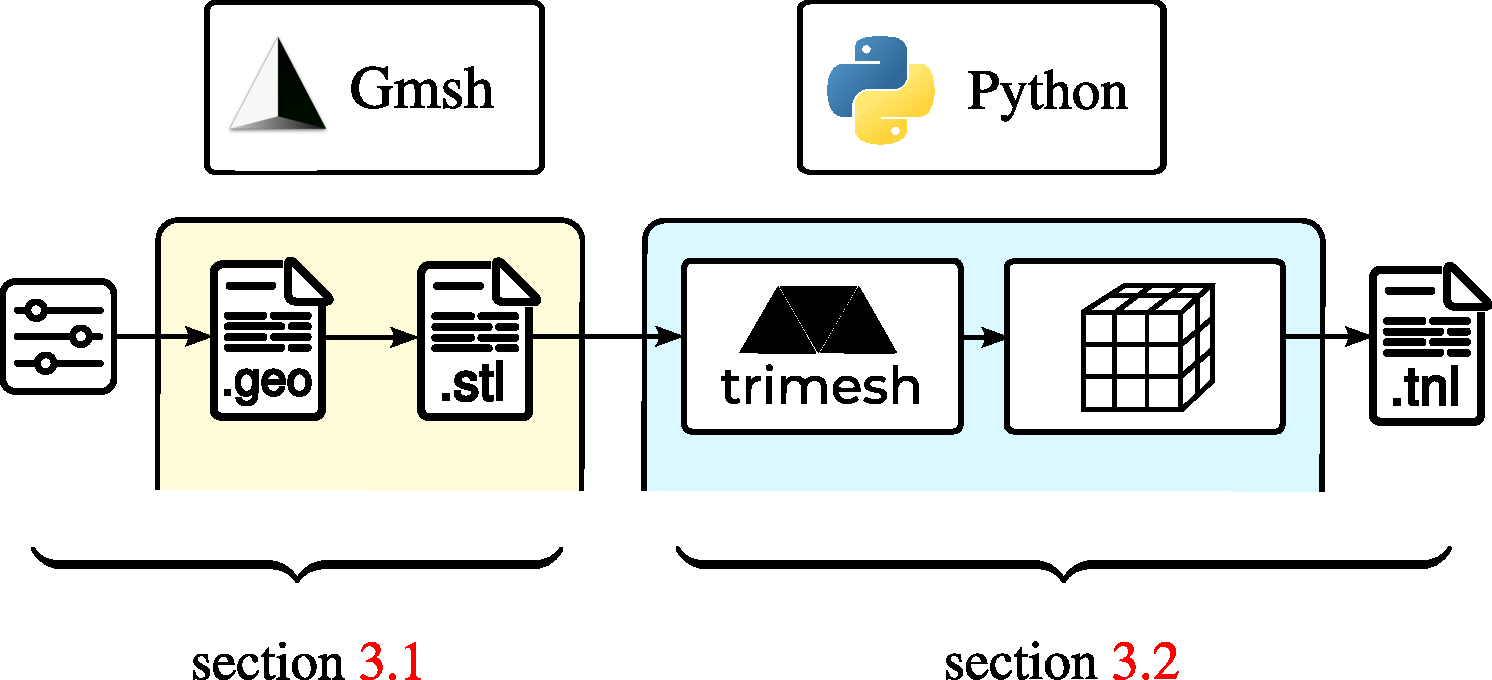
\includegraphics[width=.92\textwidth]{figures/meshgen.pdf}
	\caption{Overview of the geometry generation process. The optimization parameters are used to fill in a Gmsh \text{.geo} template file, which is used to generate an \texttt{.stl} geometry. This geometry is subsequently loaded by the Trimesh Python package and is voxelized and exported either as a \texttt{.tnl} object or a plain \texttt{.txt} file.}
	\label{fig:meshgen overview}
\end{figure}

A custom installable Python package, named \texttt{meshgen}, was implemented to encapsulate the entire process of geometry generation, from defining the geometry templates to preparing the output files for simulations. Its structure reflects the key steps in this process. The Python modules within the package are designed to handle specific tasks, such as loading and processing templates, voxelizing geometries, and providing utility functions. The modules and its specific roles in the process are discussed in detail in the following sections.

Figure  \ref{fig:meshgen structure} provides an overview of the package's structure.  The package is available upon request on Github at \href{https://github.com/buresjan/meshgen}{\texttt{https://github.com/buresjan/meshgen}}.

\begin{figure}[H]
	\centering
	\vspace{6mm}
	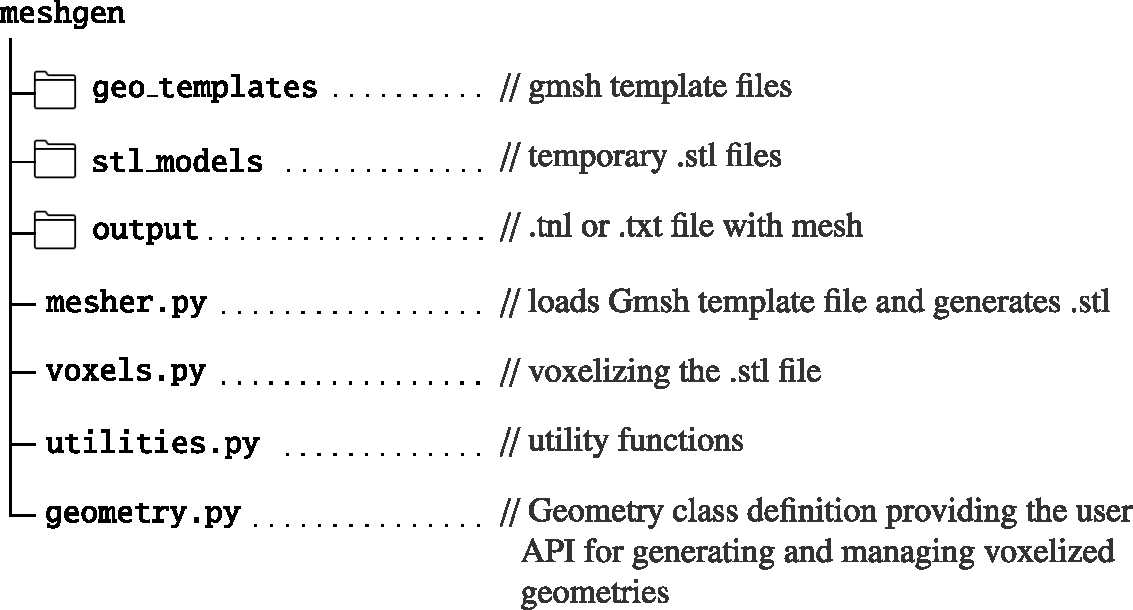
\includegraphics[width=.85\textwidth]{figures/package_overview.pdf}
	\vspace{7mm}
	\caption{Overview of the \texttt{meshgen} package structure. Each module has its specific role in the geometry generation process.}
	\label{fig:meshgen structure}
\end{figure}
\section{Template-Based Geometry Generation}

\todo[inline]{improve the mainly placeholder text, use the things we agreed upon with RF}

\subsection{Gmsh Template Files}

The geometry generation process relies on predefined Gmsh template files. These templates serve as flexible blueprints for creating a variety of geometries, with key parameters such as dimensions, resolution, and specific geometric features being dynamically filled based on the optimization parameters. The template files are structured to allow for easy modification, where placeholders represent variable values that are substituted programmatically during the optimization process.

% [Optional Figure suggestion: A snippet of a Gmsh template file, showing the placeholders and how they are replaced with actual values.]

Each Gmsh template is parameterized to accommodate variations in geometry. For example, the templates can define features such as the dimensions of the extracardiac conduit, pulmonary artery, or vena cava superior. Parameters such as the rotation angle or the mesh density are key elements that allow flexibility in the final geometry generated.

\subsection{Parameterization}

The optimization parameters dictate how the geometry templates are modified. Each parameter maps to a placeholder within the Gmsh file, which is replaced by the actual value provided during the optimization. This process ensures that each geometry is tailored precisely to the current set of optimization requirements.

One of the main challenges during parameterization is ensuring consistency across different geometries. This involves making sure that the parameters result in valid geometries that meet the required constraints for numerical simulations. Additionally, the range of allowable parameter values must be carefully managed to avoid issues such as mesh inconsistencies or geometry deformations.

\subsection{Example Workflow}

To illustrate the process, consider the generation of an extracardiac conduit. The Gmsh template defines the conduit using several geometric points, splines, and surfaces. The optimization parameters, such as the conduit diameter and length, are substituted into the template at predefined positions. Once the template is modified, Gmsh generates a 3D mesh of the conduit, which can then be further processed.

\begin{lstlisting}[language=C++]
	...
	// Define points along the axis of the upper cylinder
	Point(101) = {0.0, 0.0, LOWER_LENGTH + UPPER_LENGTH, h};
	Point(102) = {0.0, 0.0, LOWER_LENGTH, h};
	
	// Create line and wire for upper cylinder extrusion
	Line(101) = {102, 101};
	Wire(102) = {101};
	
	// Disk representing the base of the upper cylinder
	Disk(101) = {0.0, 0.0, LOWER_LENGTH + UPPER_LENGTH, UPPER_RADIUS};
	
	// Extrude the surface to form the second cylinder volume
	Extrude { Surface{101}; } Using Wire {102}
	...
\end{lstlisting}


\begin{figure}[H]
	\centering
	\vspace{6mm}
	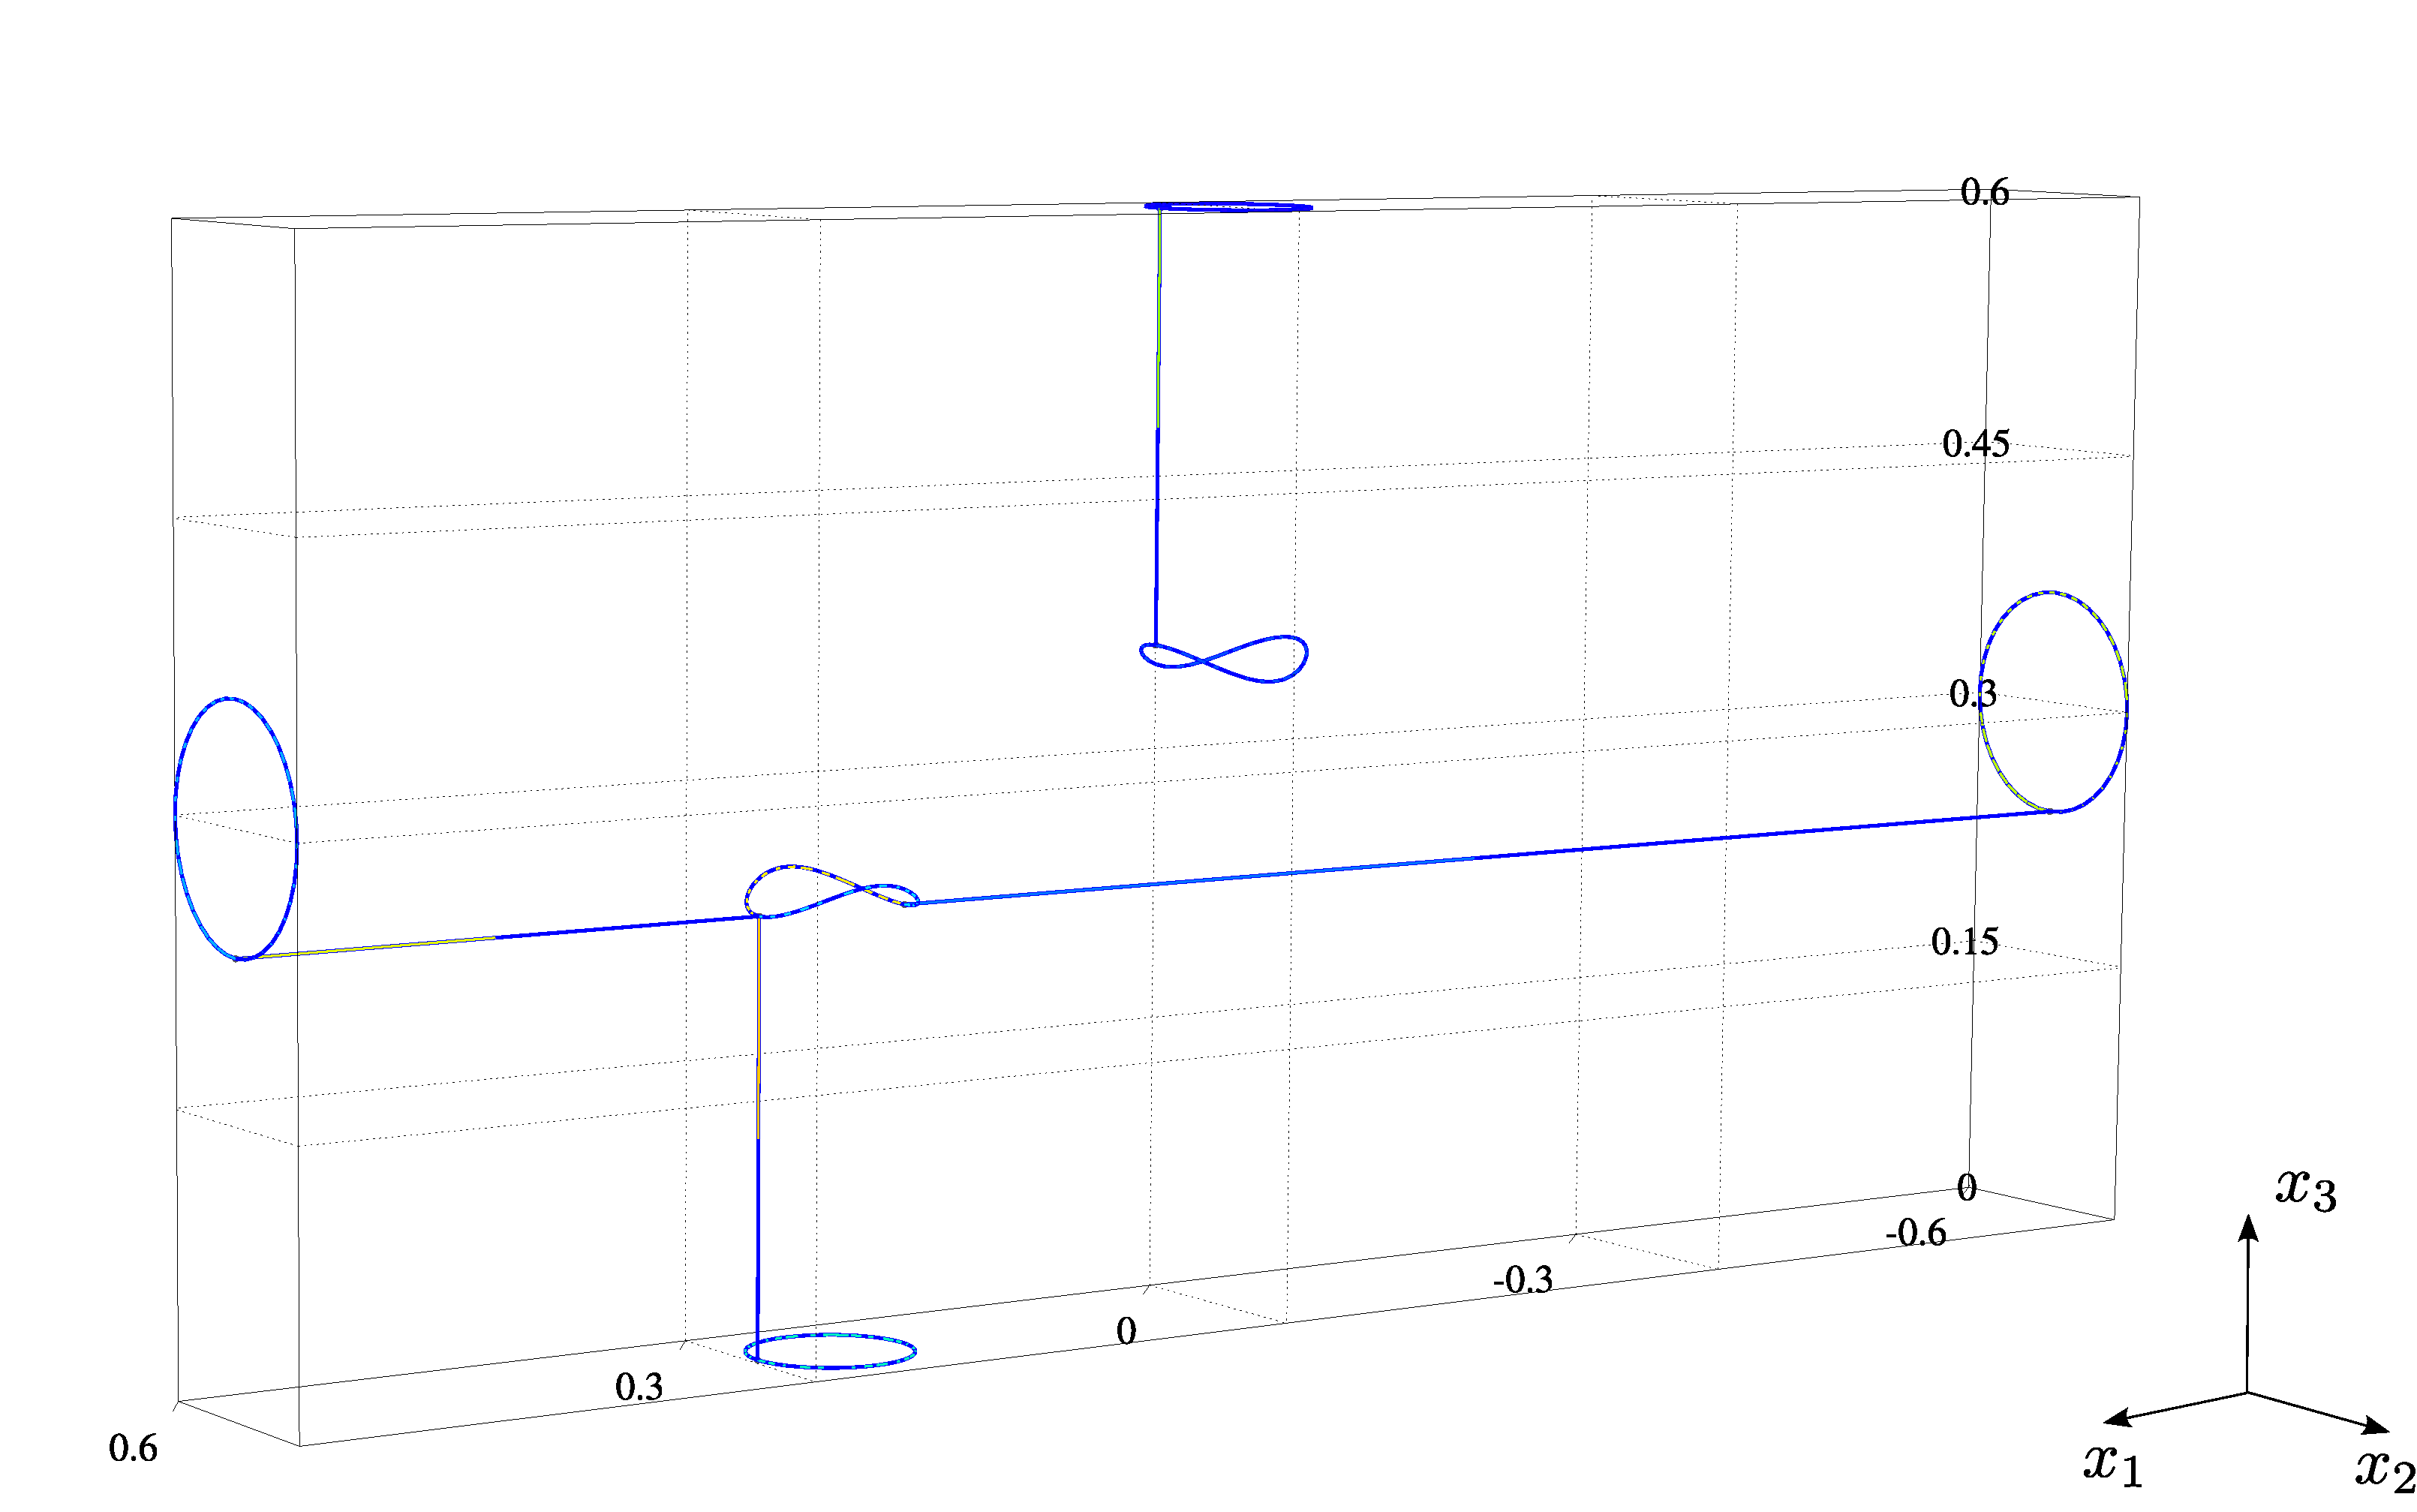
\includegraphics[width=.99\textwidth]{figures/gmsh.pdf}
	\vspace{4mm}
	\caption{Overview of the \texttt{meshgen} package.}
	\label{fig:gmsh}
\end{figure}



\begin{figure}[H]
	\centering
	\vspace{6mm}
	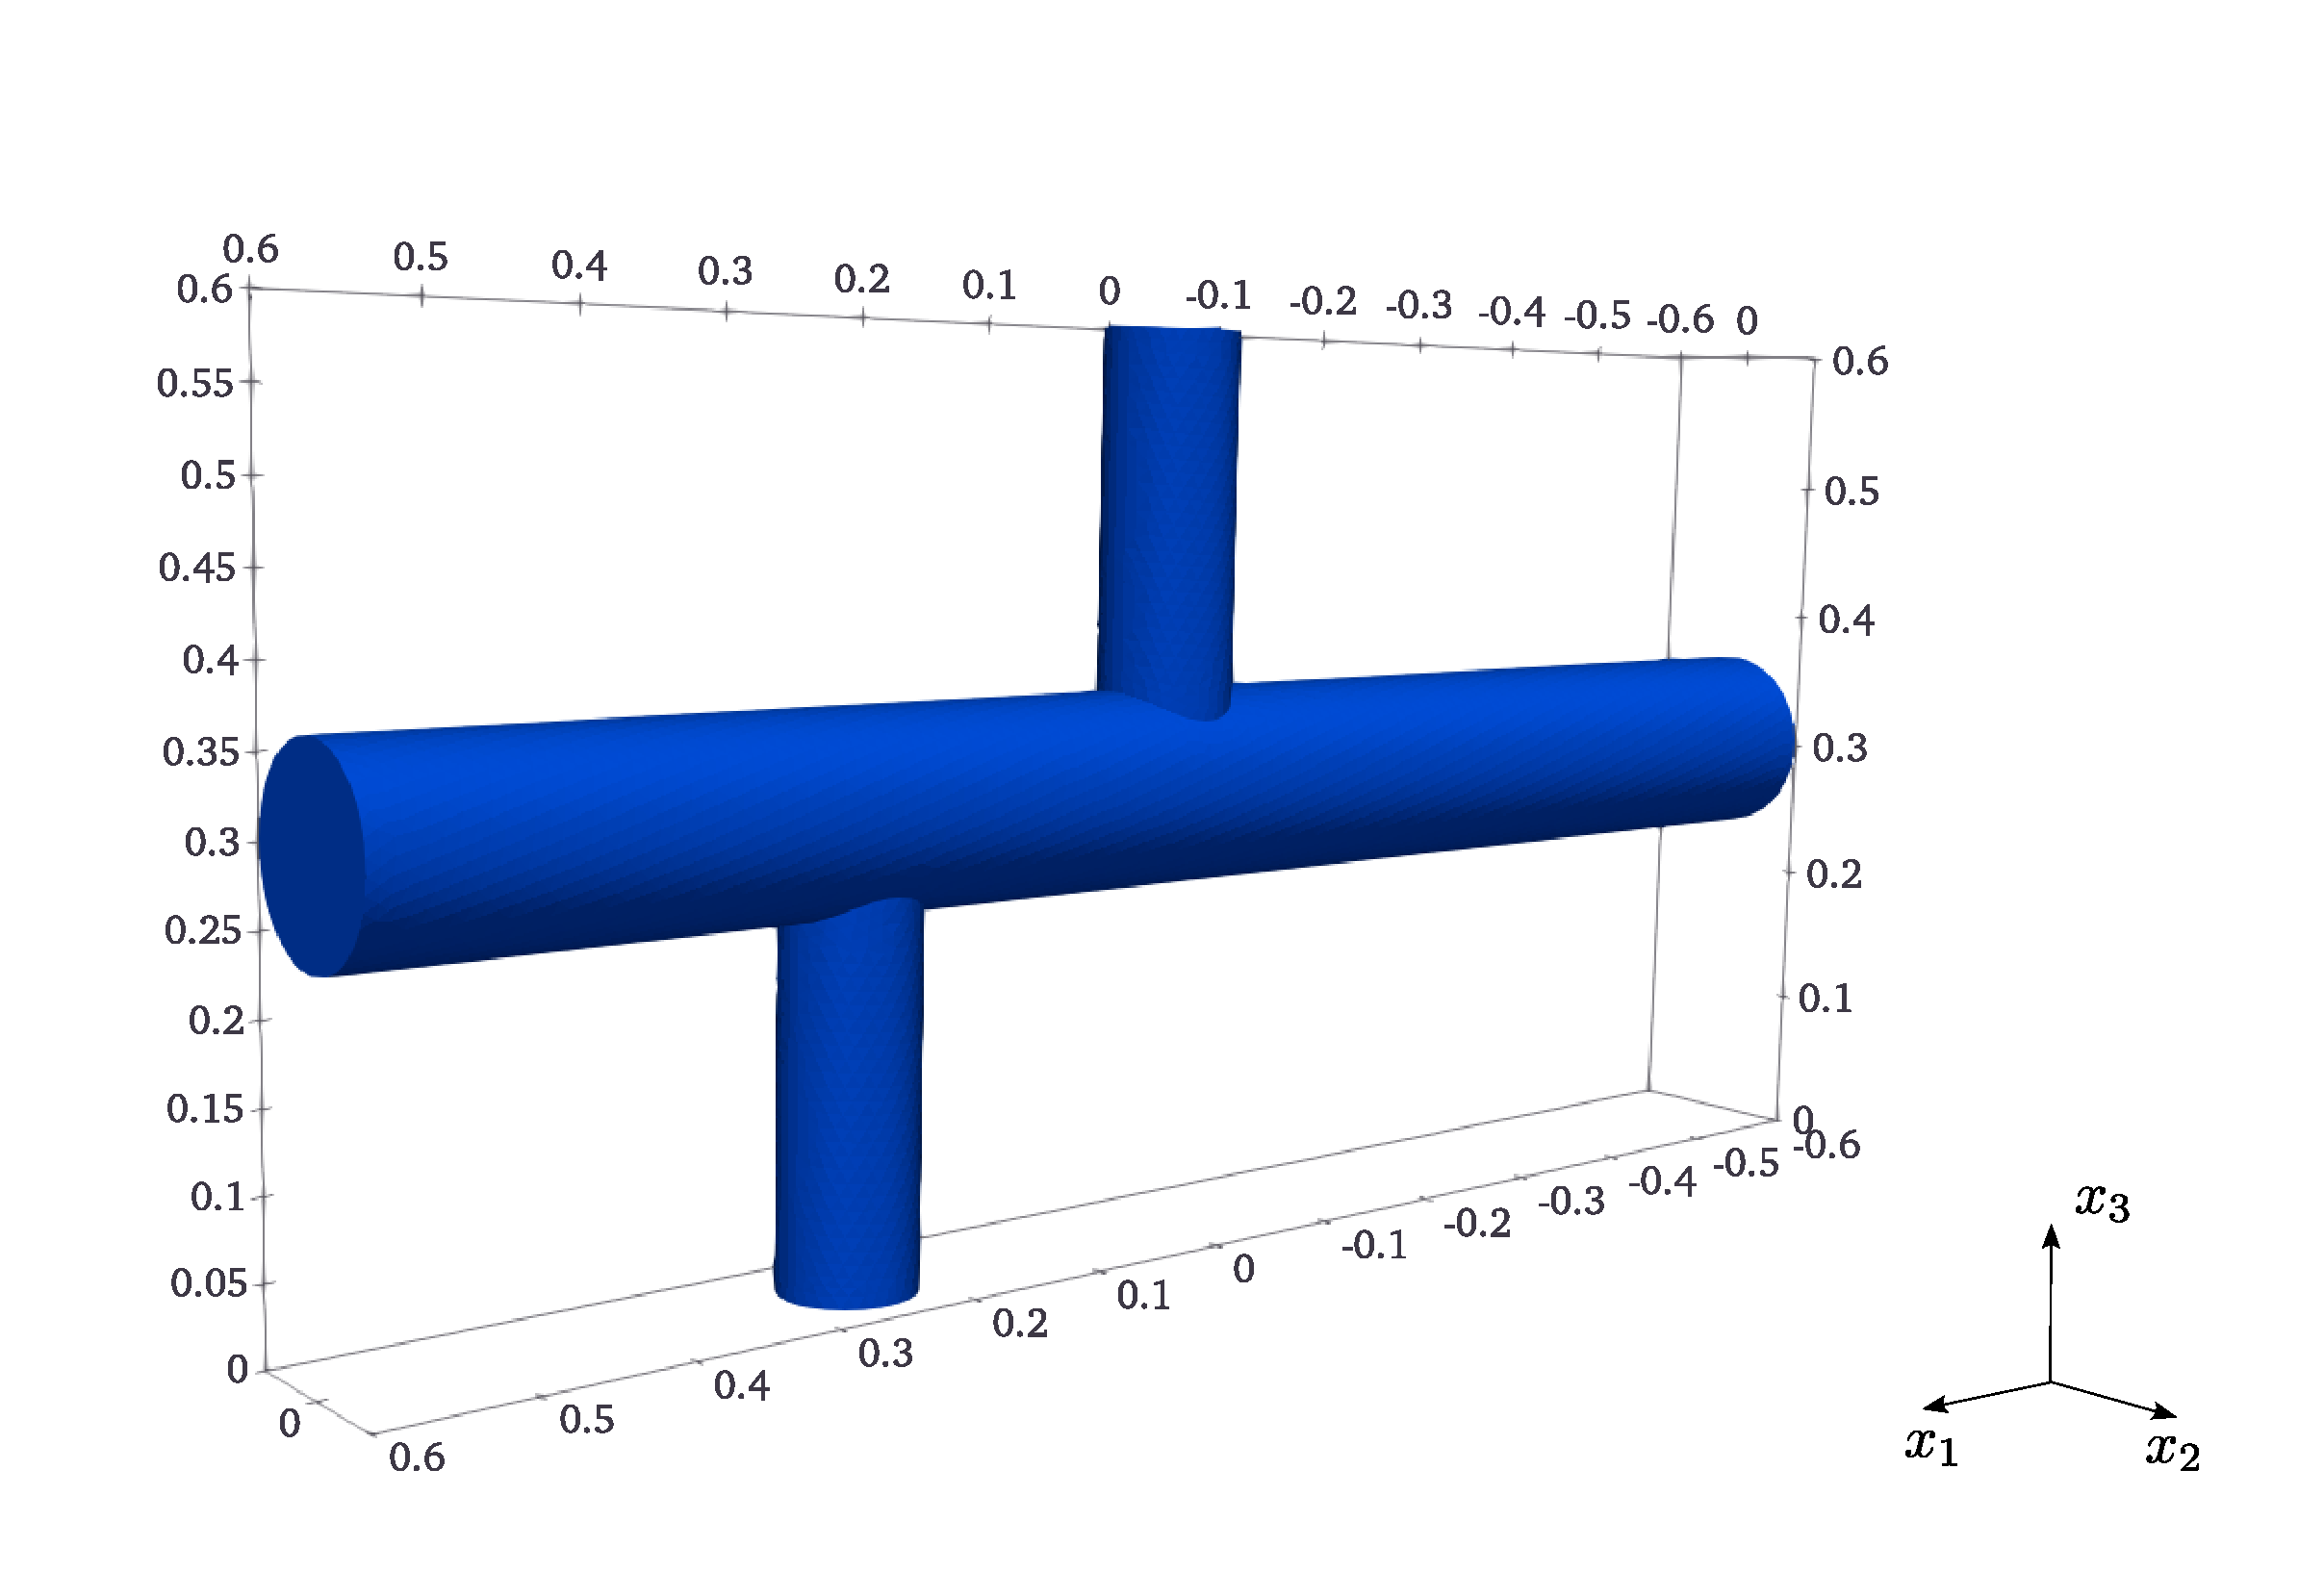
\includegraphics[width=.99\textwidth]{figures/stl.pdf}
	\vspace{4mm}
	\caption{Overview of the \texttt{meshgen} package.}
	\label{fig:stl}
\end{figure}

\section{Mesh processing}\label{mesh}

The mesh processing pipeline is designed to take raw \texttt{.stl} files generated from the geometry and convert them into a voxelized representation suitable for numerical simulations. This section describes the main steps involved in the mesh processing pipeline as illustrated in Figure \ref{fig:voxelizing}.

\begin{figure}[H]
	\centering
	\vspace{2mm}
	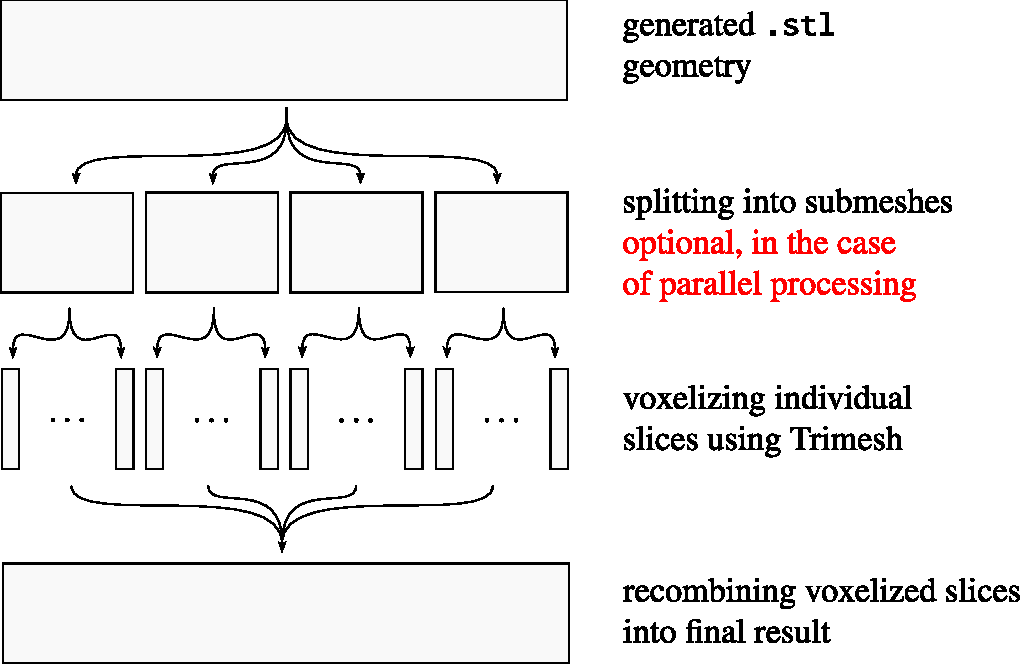
\includegraphics[width=.66\textwidth]{figures/voxelizing.pdf}
	\vspace{2mm}
	\caption{Overview of the mesh processing pipeline, including optional splitting into submeshes, voxelization of slices, and recombination into the final voxelized geometry.}
	\label{fig:voxelizing}
\end{figure}

While the Trimesh package can load and voxelize an \texttt{.stl} file in a single step, this approach becomes computationally expensive for large-scale geometries such as those used in this work. To address this issue, the mesh is split into smaller individual slices along the leading direction, which are then voxelized and recombined. On top of that, the process supports parallelization by grouping the slices into multiple independent groups.

\subsection{Parallel processing of submeshes}\label{parallelization}
 The \texttt{.stl} file can be first loaded as a mesh using the Trimesh package and then divided into smaller submeshes along its leading direction. This division reduces the computational cost by distributing the workload across multiple CPU cores, hence significantly reducing processing time.

The parallelization is achieved by using Python’s \texttt{ProcessPoolExecutor} available in the built-in \texttt{concurrent.futures} module \cite{concurrent-futures}, as shown in Listing \ref{lst:parallel}. The \texttt{ProcessPoolExecutor} allows tasks to be executed in parallel each running independently on separate CPU cores \cite{concurrent-futures}.

\begin{lstlisting}[
language=Python,
caption={Parallel processing of submeshes for voxelization.},
label={lst:parallel}]
# Parallel processing of submeshes
with ProcessPoolExecutor(max_workers=num_processes) as executor:
	# Prepare arguments for each submesh processing
	futures = [
		executor.submit(
		process_submesh,
		submsh,
		margin,
		voxel_size,
		leading_direction
		) for submsh, margin in zip(submeshes, margins)
	]
	
	# Collecting results with progress display
	comps = [
		future.result() for future in 
		tqdm(futures, total=len(submeshes), desc="Voxelizing")
	]
\end{lstlisting}

\subsection{Voxelization and recombination of slices}\label{voxelizing and recombining}

The mesh, whether processed as a whole or divided into submeshes (if parallelization is used), is split into individual slices based on thickness that is defined by the user. Each slice is then converted into a voxelized representation using the Trimesh package, which provides a tool for voxelizing 3D geometries, as shown in Listing \ref{lst:voxelize}.

\begin{lstlisting}[
	language=Python,
	caption={Voxelization of a mesh slice using the Trimesh package \cite{trimesh}.},
	label={lst:voxelize}]
def voxelize_elementary(mesh, voxel_size):
	# Voxelize mesh with the specified voxel size
	# In this case, the mesh represents an elementary slice
	return mesh.voxelized(voxel_size).matrix
\end{lstlisting}

Finally, the voxelized slices are recombined using the \texttt{numpy.concatenate} function \cite{numpy} along the leading direction to form the final geometry ready for simulation.


\subsection{The \texttt{Geometry} class: a user-friendly interface}

The \texttt{Geometry} class serves as a high-level interface that encapsulates the entire process of mesh generation. It provides users with control over the voxelization process, including options to define the slice thickness and distribute the workload into parallel tasks. The class also supports visualization and file export in multiple formats.

The \texttt{Geometry} class supports the following key functionalities:
\begin{itemize}
	\item \textbf{Voxelization}: Converts the geometry into a voxelized representation based on a Gmsh \texttt{.geo} template as discussed in \ref{voxelizing and recombining}. 
	
	\item \textbf{Parallel Processing}: Allows users to split the geometry into slices paramater) and process them in parallel across multiple CPU cores as discussed in \ref{parallelization}.
	
	The \texttt{split} parameter determines the number of slices into which the mesh is divided along its leading direction. The \texttt{num\_processes} parameter specifies the number of groups into which the slices are distributed, with each group processed on a separate CPU core. 
	
	\item \textbf{Mesh Exporting}: Exports the voxelized mesh as binary NumPy object (\texttt{.npy}), plain text file (\texttt{.txt}), or LBM simulation-compatible \texttt{.tnl} format. Exporting in the \texttt{.tnl} format is achieved using the PyTNL package \cite{pytnl}, which provides Python bindings for TNL.
	
	\item \textbf{Visualization}: Visualizes the voxelized geometry, primarily for debugging purposes. Visualization is implemented using the Mayavi Python package \cite{mayavi}, which allows inspecting geometries in an interactive 3D environment. An example visualization, generated using the \texttt{.geo} template file from Appendix \ref{appendix A}, is shown in Figure \ref{fig:visualization}.
\end{itemize}

\begin{figure}[H]
	\centering
	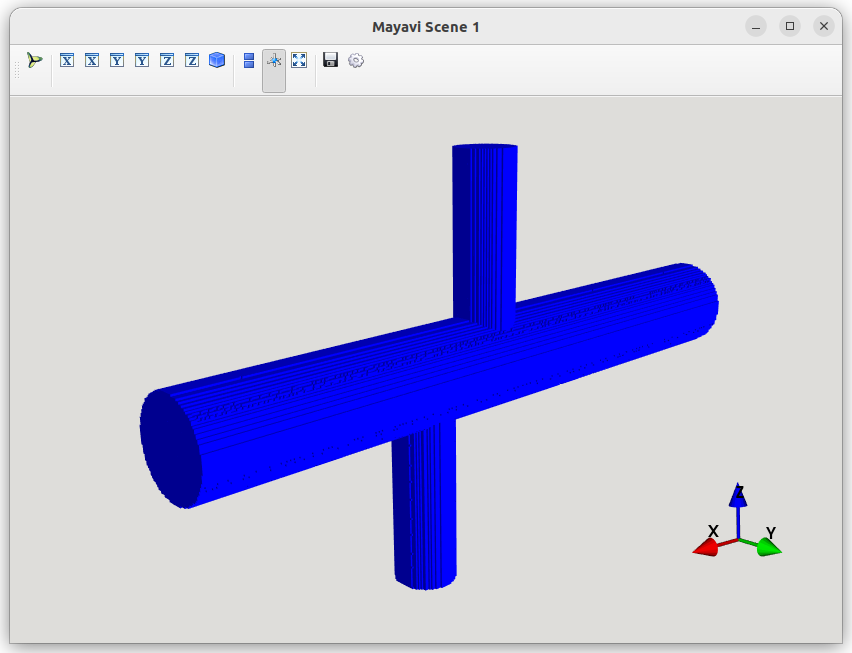
\includegraphics[width=.7\textwidth]{figures/mayavi.png}
	\caption{Visualization of the voxelized geometry using the Mayavi package \cite{mayavi}.}
	\label{fig:visualization}
\end{figure}


Finally, the following code demonstrates the usage of the \texttt{Geometry} class, from defining the object to exporting the voxelized geometry in multiple formats and visualizing it.

\begin{lstlisting}[
	language=Python,
	caption={Example usage of the \texttt{Geometry} class.},
	label={lst:geometry}
	]
from meshgen.geometry import Geometry
	
# Initialize a Geometry instance with parameters
geom = Geometry(
	name="junction_1d",  # name of the .geo template file
	resolution=8,        # desired resolution for the LBM simulation
	split=1024,          # slice thickness; mesh is split into 1024 
						 # slices
	num_processes=8,     # distribute slices into 8 groups, each
						 # processed on a separate CPU core
	offset=0.02,		 # any optimization parameters specific to
						 # the problem
	expected_in_outs={"W", "E", "S", "N"} # list of the parts of the
										  # computational domain that
										  # are expected to include 
										  # the inlets and outlets;
										  # for practical purposes
)
	
# Generate the voxel mesh
geom.generate_voxel_mesh()

# Save the voxel mesh in various formats
geom.save_voxel_mesh("voxel_mesh.npy")
geom.save_voxel_mesh_to_text("voxel_mesh.txt")
geom.save_voxel_mesh_to_tnl("voxel_mesh.tnl")

# Visualize the voxelized geometry
geom.visualize()
\end{lstlisting}

\chapter{Mathematical optimization}\label{optimization}

%Mathematical optimization, also known as mathematical programming, is a broad field that covers various disciplines, including linear and nonlinear optimization, convex programming, integer programming, and more. The goal of this chapter is to summarize the key concepts and techniques relevant to the scope of this work. Specifically, we will focus on methods for solving optimization problems with constraints and those where the objective function is generally unknown and its evaluation is computationally expensive. Classic methods applicable to unconstrained optimization, such as the Davidon-Fletcher-Powell \cite{Fletcher1963} and Broyden-Fletcher-Goldfarb-Shanno \cite{broyden1970} algorithms, while fundamental, fall outside the scope of this work and details on these methods can be found for instance in \cite{Bert}.
%
%%This chapter focuses on methods that address the specific challenges posed by constrained and generally unknown objective functions. First, a general optimization problem is defined, followed by an introduction to basic techniques for solving constrained problems. Next, black-box optimization methods are discussed. Finally, the proposed optimization framework, including its components and their interconnections, is presented in detail.
%
%This chapter focuses on methods that address the specific challenges posed by constrained and generally unknown objective functions. First, a general optimization problem is defined. Next, black-box optimization methods are discussed. Finally, the proposed optimization framework, including its components and their interconnections, is presented in detail.

%\section{General optimization problem}

Let $m, n, q \in \mathbb{N}$. Define the continuous functions $f : \mathbf{D} \rightarrow \mathbb{R}$, $ \vec{g} : \mathbf{D} \rightarrow \mathbb{R}^m$, $ \vec{h} : \mathbf{D} \rightarrow \mathbb{R}^q $, where $ \mathbf{D} = \mathrm{Dom} \, (f) \cap \mathrm{Dom} \, (\vec{g}) \cap \mathrm{Dom} \, (\vec{h})$, i.e., $ \mathbf{D} $ is the intersection of the domains of the given functions. Next, define the set

\begin{equation}\label{eq:feasible solution}
	\mathbf{X} = \big\{ \vec{x} \in \mathbf{D} \subseteq \mathbb{R}^n \ | \ \vec{g} (\vec{x}) \leq \vec{0} \wedge \vec{h} (\vec{x}) = \vec{0} \, \big\},
\end{equation}
where the inequality $ \vec{g} \leq \vec{0} $ and equality $ \vec{h} = \vec{0} $ are understood component-wise. The general goal of mathematical optimization is to solve the problem
\begin{equation}\label{eq:basic problem}
	\min_{\vec{x} \in \mathbf{X}} f(\vec{x}).
\end{equation}

The function $f$ being minimized is called the objective function, $\mathbf{D}$ is referred to as the domain of the problem, and $\mathbf{X}$~is called the set of feasible solutions of the problem \cite{Bert}. Note that, henceforth, $f$ denotes only the objective function and not the distribution function discussed in Chapter \ref{lbm}.

When classifying optimization problems, we refer to what are known as constraints. These are determined by the definition of the set $ \mathbf{X} $, i.e., the equality and inequality conditions for the functions $ \vec{g} $~and $ \vec{h} $, and by the domain $ \mathbf{D} $. Constraints defined by $ \vec{g} (\vec{x}) \leq \vec{0} \wedge \vec{h} (\vec{x}) = \vec{0} $ are called explicit constraints, while those determined by the domain $ \mathbf{D} $ are called implicit constraints.
\newpage
The optimal solution of the problem \eqref{eq:basic problem} is denoted by $ \vec{x}^{\star} \in \mathbf{X} $ and is defined as
\begin{equation}
	\vec{x}^{\star} = \operatorname*{argmin}_{\vec{x} \in \mathbf{X}} \, f(\vec{x}).
\end{equation}
Note that the optimal solution may not be unique, and we refer to the set of all optimal solutions as the optimal set. It is also important to recognize that the search for an optimal solution can equivalently be formulated as finding the maximum of the function $ -f$ over the same set $ \mathbf{X}$, enabling the use of the same techniques for solving maximization problems \cite{Bert, non-linear-textbook}.
%%\section{Solving constrained problems}\label{constrained}
We will now consider the problem \ref{eq:basic problem}, where the set of admissible solutions is given by \ref{eq:admissible solution}. In this section, we describe how to generally solve this problem by converting it into a sequence of unconstrained optimization problems. There exist several other methods for solving constrained problems, but here we will focus on the penalty and the barrier methods.

\subsection{Penalty methods}\label{penalty method}
As mentioned earlier, penalty methods convert constrained optimization problems into unconstrained ones. The fundamental principle of penalty methods is to incorporate the conditions that define the set of admissible solutions by adding a penalty term to the objective function, which reflects the degree of violation of those conditions \cite{Bert}. The penalty function is defined as a continuous scalar function on $ \mathbb{R}^n $ that satisfies

\begin{align}
	\begin{split}
		p(\vec{x}) &= 0, \ \ \forall \vec{x} \in \mathbf{X},\\[6pt]
		p(\vec{x}) &> 0, \ \ \text { otherwise. }
	\end{split}
\end{align}
A typical choice for the penalty function is, e.g.,
\begin{equation}\label{eq:penalty function}
	p (\vec{x}) = \sum_{j=1}^{m} \left( \, \max  \left\{ \, g_j (\vec{x}), 0 \, \right\} \, \right)^2 + \sum_{j=1}^{q} h_j (\vec{x})^2.
\end{equation}
Using the penalty function $ p $, we construct the modified objective function
\begin{equation}\label{eq:cost function with penalty}
	\phi (\vec{x}, r) = f (\vec{x}) + r p(\vec{x}),
\end{equation}
where $ r > 0 $ is called the penalty coefficient \cite{Bert}. From the definition of the penalty function, it can be seen that the values of the modified objective function $ \phi (\vec{x}, r)$ differ from the original function $ f $ only for such $ \vec{x} $ that violate the specified condition.

To solve the constrained problem, we iteratively construct a new term in an increasing sequence of penalty coefficients $ r_1, r_2, \dots$, for which we solve the unconstrained optimization problem for the modified function $ \phi (\vec{x}, r_k)$. The optimal solution $ \vec{x}_k $ of this unconstrained problem is then used as the starting point for the next iteration. This process is repeated until the condition $ r_k p(\vec{x}_k) < \varepsilon$ for some $ \varepsilon > 0$ is satisfied. When this condition is met, $ \vec{x}_k $ can be considered a sufficiently accurate approximation of the solution to the constrained problem. It should be noted that penalty methods allow searching for an optimal solution outside the set of admissible solutions during the iterations \cite{non-linear-textbook}, and thus are categorized as exterior point methods. A key assumption of penalty methods is that the domain of the problem satisfies $ \mathbf{D} = \mathbb{R}^n $.

The construction of the sequence of penalty parameters and the principle of the penalty method are illustrated in Figure~\ref{fig:penalty} on a trivial example of minimizing the function $ f(x) = 0.5x $ with the constraint $ g(x) = 4 - x \leq 0 $. The modified objective function in this case takes the form
\begin{equation}
	\phi (x, r) = 0.5x + r \left(\max  \left\{ \,  4-x, 0 \right\}\right)^2.
\end{equation}
\begin{figure}[H]
	\vspace{-2.25cm}
	\centering
	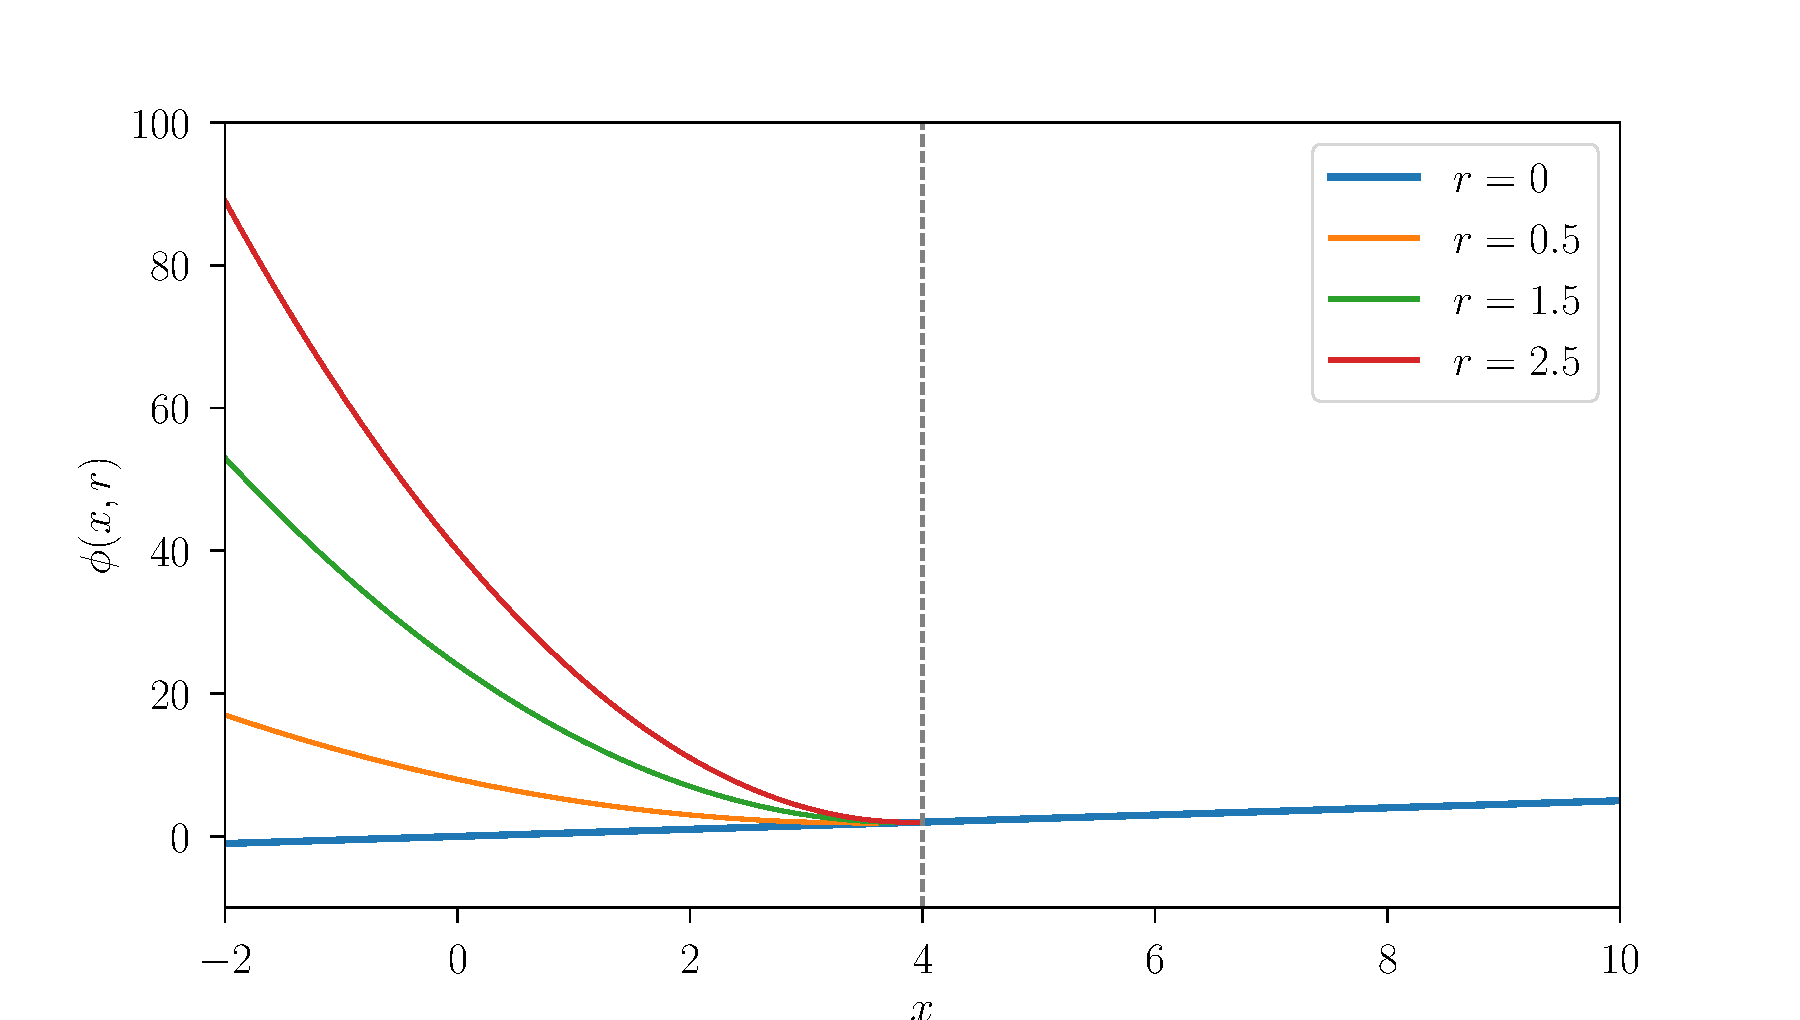
\includegraphics[width=0.9\textwidth]{figures/penalty.pdf}
%	\vspace{0.2cm}
	\caption{An illustration of the penalty method applied to minimizing the function $ f(x) = 0.5x $ with the constraint $ g(x) = 4 - x \leq 0 $. Different shapes of the modified objective function $ \phi (x, r) $ depending on the value of the penalty parameter $ r $ are distinguished by color. The condition defining the set of admissible solutions is indicated by the gray dashed line. The set of admissible solutions lies in the half-plane to the right of this gray dashed line.}
	\label{fig:penalty}
\end{figure}


\subsection{Barrier method}\label{barrier method}
The barrier method operates on a principle similar to that of the penalty method, but its main difference is that, during the iterative process of finding an optimal solution to a constrained problem, it ensures that the solution estimates always remain within the interior of the feasible set, which is defined as
\begin{equation}
	\mathbf{X}^{\mathrm{o}} = \left\{ \vec{x} \in \mathbf{D} \subseteq \mathbb{R}^n \ \middle| \ \vec{g}(\vec{x}) < \vec{0} \right\}.
\end{equation}
Methods that satisfy this condition are generally referred to as interior-point methods \cite{non-linear-textbook}.

As with penalty methods, we account for the conditions defining the feasible set by adding a new term to the objective function, which reflects the degree to which these conditions are violated. The barrier function $ B $ is a continuous scalar function on $ \mathbf{X}^{\mathrm{o}} $ that satisfies the condition
\begin{equation}
	(\exists j \in \{1,2,\dots,m\})(\lim\limits_{\substack{\vec{x} \to \vec{y} \\ \mathbf{X}^{\mathrm{o}}}} g_j (\vec{x}) = 0) \Rightarrow \lim\limits_{\substack{\vec{x} \to \vec{y} \\ \mathbf{X}^{\mathrm{o}}}} B (\vec{x}) = + \infty.
\end{equation}
A typical choice for the barrier function is the logarithmic barrier function
\begin{equation}\label{eq:log barrier function}
	B (\vec{x}) = -\sum_{j=1}^{m} \ln \left( - g_j (\vec{x}) \right),
\end{equation}
or alternatively, the reciprocal barrier function
\begin{equation}\label{eq:reciprocal barrier function}
	B (\vec{x}) = -\sum_{j=1}^{m} \frac{1}{g_j (\vec{x})}.
\end{equation}
Using the barrier function $ B $, similar to the penalty methods, we construct the modified objective function
\begin{equation}\label{eq:cost function with barrier}
	\phi (\vec{x}, r) = f (\vec{x}) + r B(\vec{x}),
\end{equation}
where $ r > 0 $ is a chosen parameter \cite{non-linear-textbook}.

To solve the constrained problem using the barrier method, at each iteration we construct a new term in a strictly decreasing sequence of positive parameters $ r_1, r_2, \dots$, for which we solve the unconstrained optimization problem for the modified function $ \phi (\vec{x}, r_k)$. The vector $ \vec{x}_k  = \operatorname*{argmin}_{\vec{x} \in \mathbf{X}^\mathrm{o}} (f(\vec{x}) + r_k B(\vec{x})) $, obtained by optimizing the unconstrained problem, is used as the starting point for the next iteration. This process is repeated until the condition $ r_k < \varepsilon$ for some chosen $ \varepsilon > 0$ is satisfied, at which point $ \vec{x}_k $ is considered a sufficient approximation to the solution of the constrained problem \cite{non-linear-textbook}.

The construction of the parameter sequence $ (r_k)_{k \in \mathbb{N}} $ and the principle of the barrier method are illustrated in Fig.~\ref{fig:barrier} using the example of minimizing the function $ f(x) = 0.5x $ with the constraint $ g(x) = 4 - x \leq 0 $ and the choice of the reciprocal barrier function. The modified objective function in this case is
\begin{equation}
	\phi (x, r) = 0.5x - \frac{r}{4-x}.
\end{equation}

\begin{figure}[H]
	\centering
	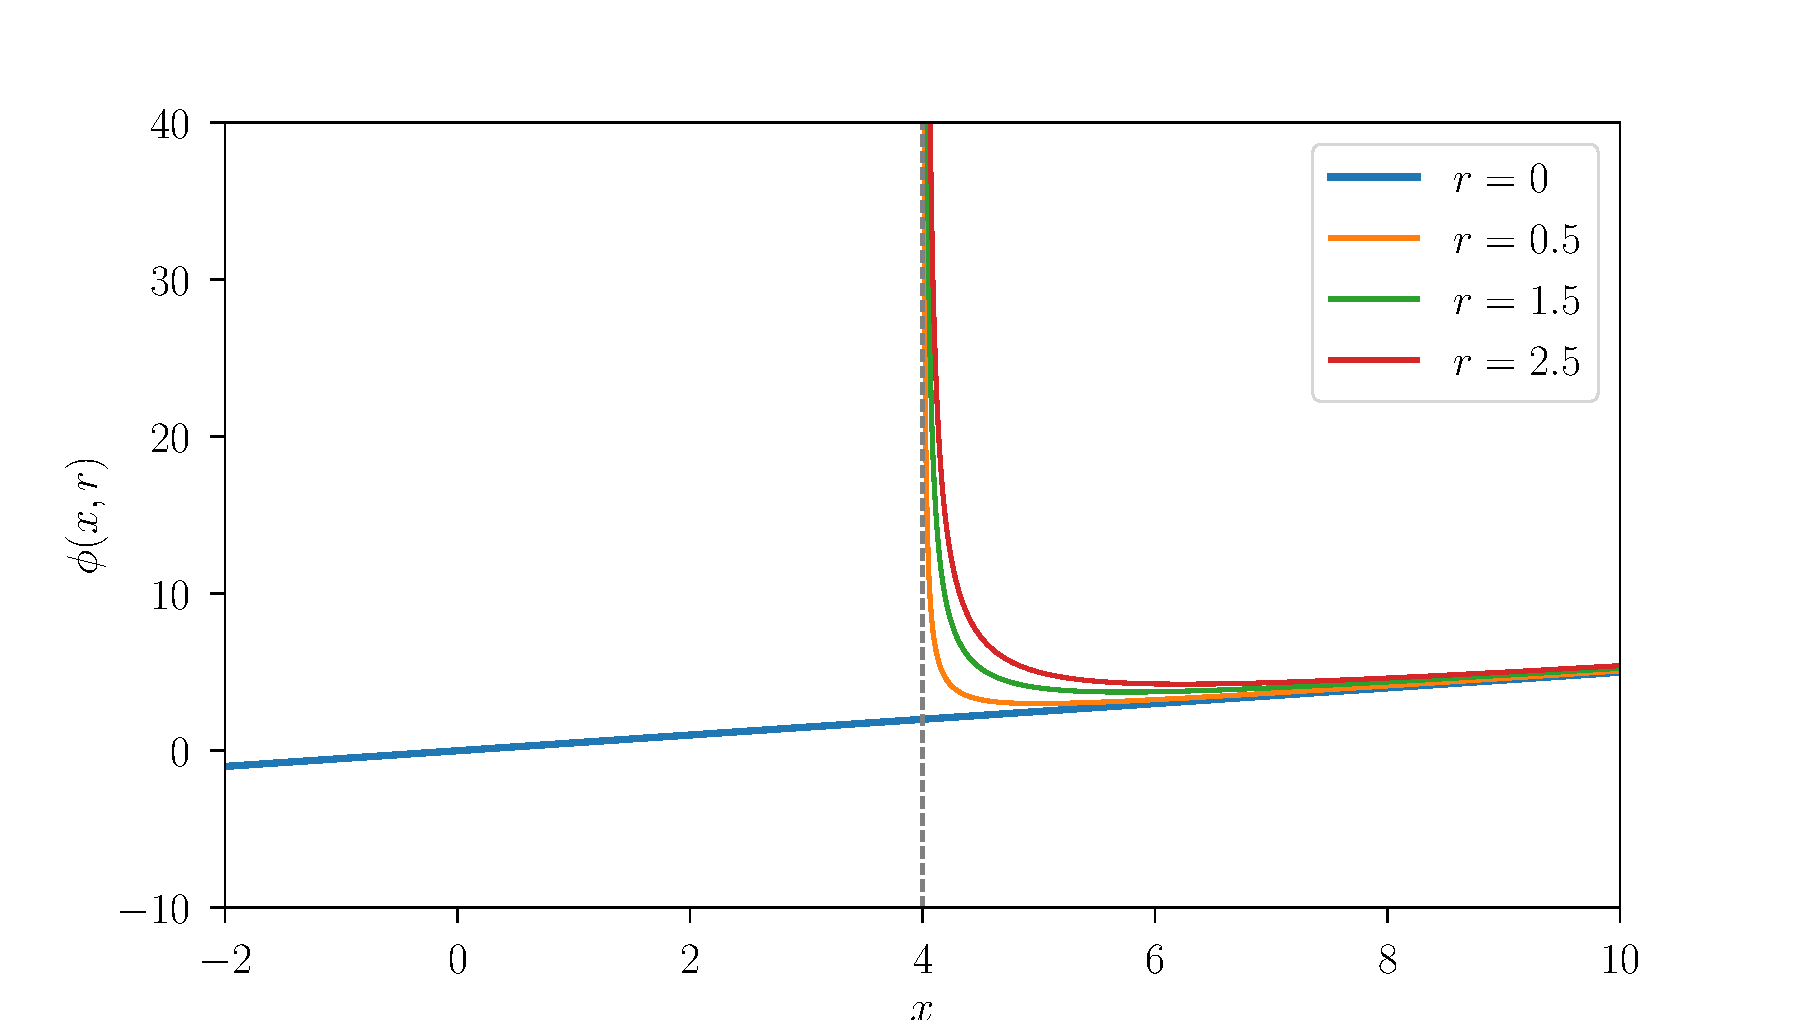
\includegraphics[width=0.9\textwidth]{figures/barrier.pdf}
	\caption{An illustration of the barrier method applied to minimizing the function $ f(x) = 0.5x $ with the constraint $ g(x) = 4 - x \leq 0 $. Different shapes of the modified objective function $ \phi (x, r) $ depending on the value of the barrier parameter $ r $ are distinguished by color. The condition defining the set of feasible solutions is indicated by the gray dashed line. The set of feasible solutions lies in the half-plane to the right of this gray dashed line.}
	\label{fig:barrier}
\end{figure}

Finally, we mention the choice of the barrier function $ B_{\infty} $ used to define the so-called extreme barrier function, as the modified objective function is called with this choice \cite{BBO-textbook}. This barrier function mirrors the asymptotic behavior of the aforementioned barrier functions and is given by
\begin{align}
	\begin{split}
		B_{\infty}(\vec{x}) &= 0, \ \ \forall \vec{x} \in \mathbf{X},\\[6pt]
		B_{\infty}(\vec{x}) &= +\infty, \ \ \text{otherwise.}
	\end{split}
\end{align}
The modified objective function (extreme barrier function) is then given by
\begin{align}\label{eq:extreme barrier}
	\begin{split}
		f_{\infty}(\vec{x}) &= f(\vec{x}) , \ \ \forall \vec{x} \in \mathbf{X},\\[6pt]
		f_{\infty}(\vec{x}) &= +\infty, \ \ \text{otherwise.}
	\end{split}
\end{align}
%\section{Black-box optimization}\label{black-box}
In practice, we often need to optimize an objective function $f$ whose exact form and derivative are unknown. This is common in numerical simulations, where the function can only be evaluated at specific points. Moreover, evaluating the function at a point may be difficult, time-consuming, or computationally expensive. As a result, standard optimization algorithms are not well-suited for these problems.

The discipline that deals with problems where the objective function (or constraints) is given by a so-called black-box\footnote{In programming, a black-box refers to a system whose internal mechanisms are unknown to the user. This means that the user generally has access only to the system’s input and output \cite{BBO-textbook}.}, is called black-box optimization (hereafter referred to as BBO). In BBO, it is typically not assumed that the objective function is continuous or differentiable \cite{BBO-textbook, derivative-free-review, two-decades}.

It is worth noting that in the literature, black-box optimization is often confused with derivative-free optimization (DFO), which encompasses methods and techniques for objective functions whose derivatives are unknown or difficult to compute \cite{BBO-textbook, derivative-free-review, Kramer2011}. These two disciplines share many common characteristics, but they differ primarily in that, within DFO, the formula for calculating the derivative of the objective function may still be known. Furthermore, BBO includes heuristic methods, whereas DFO focuses mainly on methods that can be reliably analyzed mathematically in terms of convergence and stopping criteria, which is often not possible for BBO methods \cite{BBO-textbook}. Therefore, although the terms BBO and DFO are often used interchangeably, in this work, we will treat them as two distinct disciplines \cite{BBO-textbook}.

Additionally, it should be noted that various classifications of methods within BBO can be found in the literature. In this work, we will adhere to the classification presented in \cite{BBO-textbook}, distinguishing between heuristic methods, direct search methods, and methods based on surrogate models. Each of these classes will be briefly described in this section.


\subsection{Heuristic Methods}\label{heuristic}
Heuristic optimization methods often rely on different predefined rules or even trial and error when seeking the solution of an optimization problem. These methods usually do not guarantee optimal solutions, but they are often effective for finding near-optimal results in a reasonable amount of time. Heuristic methods include genetic algorithms, detailed in \cite{BBO-textbook}, along with various other heuristic approaches.

In this section, however, we will focus on a different widely used heuristic method, the Nelder-Mead method, also known as the simplex method\footnote{A simplex in $ \mathbb{R}^n $ is defined as a bounded convex polytope (a generalization of a polyhedron to any dimension) with a non-empty interior and exactly $ n+1 $ vertices \cite{BBO-textbook}.}\footnote{The term "simplex method" more commonly refers to the algorithm used to find the optimal solution in linear programming. This algorithm was developed by George Dantzig \cite{Dantzig1990}.}\cite{Nelder1965}.

The Nelder-Mead method finds a solution to an optimization problem by iteratively constructing simplexes. The process begins by initializing a starting simplex. The objective function is then evaluated at each vertex of this simplex. In each subsequent iteration, the simplex is transformed in order to move closer to the position of the sought stationary point of the objective function. The transformation of the simplex involves manipulating its points using predefined operations -- expansion, reflection, contraction (inner and outer), and shrinking, which are schematically illustrated in Figure~\ref{fig:NM operations}. 

\begin{figure}[H]
	%	\vspace{5mm}
	\centering
	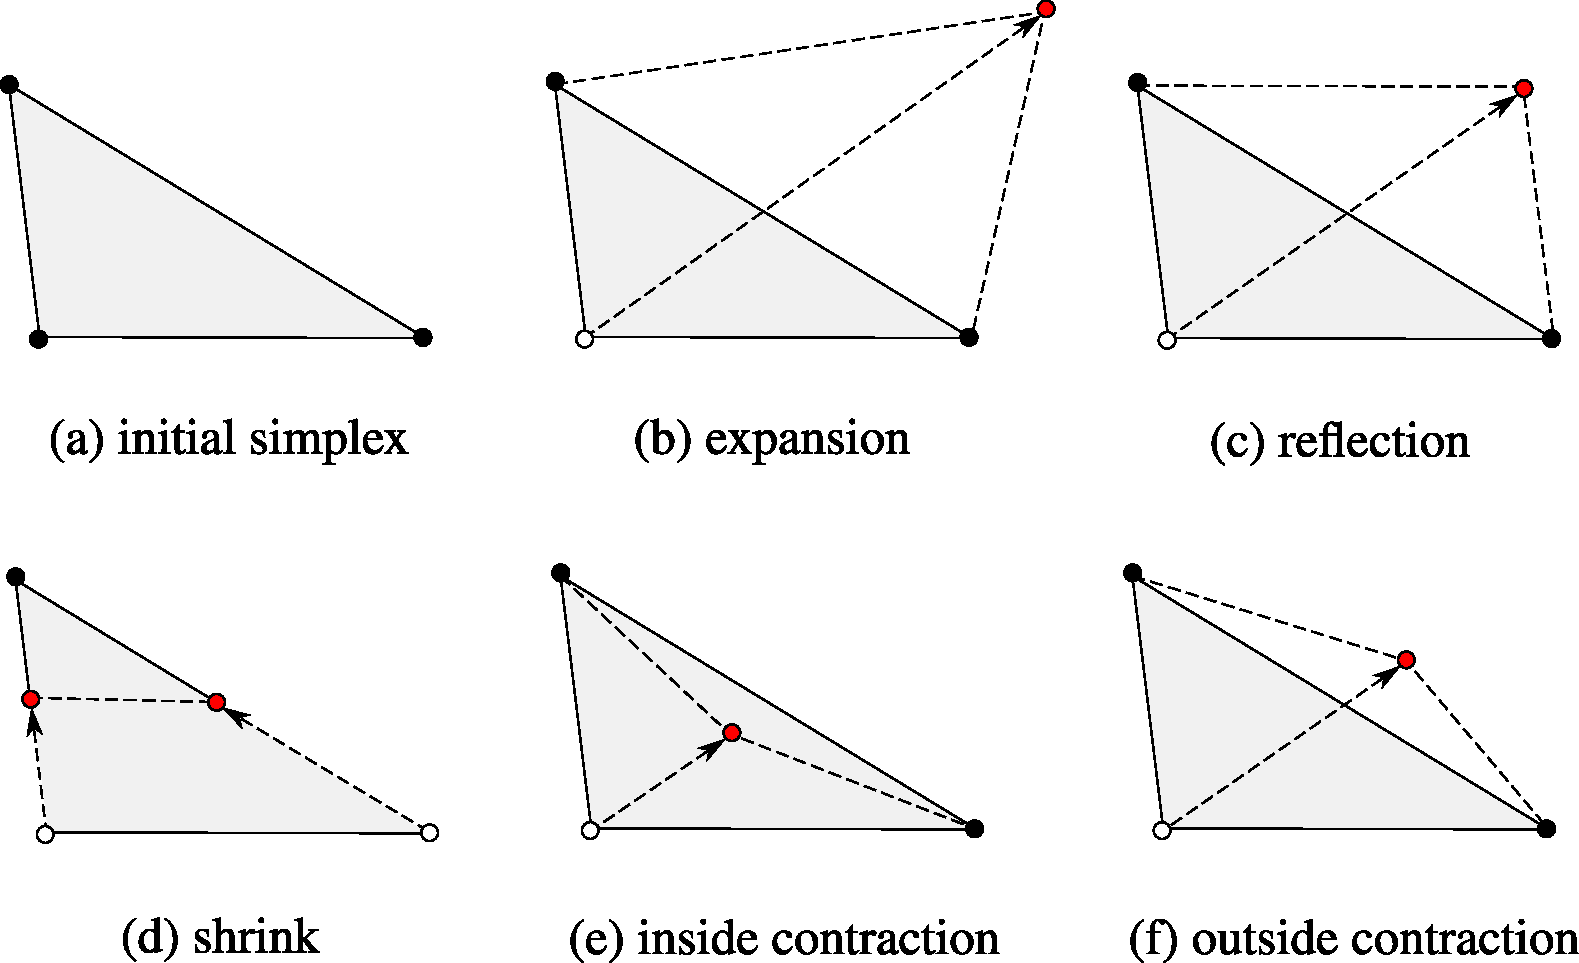
\includegraphics[width=0.96\textwidth]{figures/neldermead.pdf}
	\vspace{2mm}
	\caption{A schematic representation of the operations used to transform simplexes in the Nelder-Mead method. The vertices generated by applying each operation are shown in red. For clarity, the operations are depicted in $ \mathbb{R}^2 $.}
	%	\vspace{2mm}
	\label{fig:NM operations}
\end{figure}

The transformations performed during each iteration are determined by comparing the function values at the vertices of the simplex. The newly formed simplex shares either exactly one vertex or exactly $ n $ vertices with the simplex from the preceding iteration. The algorithm continues to iteratively transform the simplex until a stopping condition (specified by the user) is met \cite{BBO-textbook}. Details of the Nelder-Mead method, including the algorithm's description and the choice of stopping condition, are discussed in \cite{BBO-textbook, derivative-free-review, Nelder1965}. The full Nelder-Mead method algorithm is presented in Algorithm~\ref{neldermead}.

\begin{algorithm}
	\caption{Nelder-Mead algorithm}\label{neldermead}
	\begin{algorithmic}[1]
		\Require Initial simplex $S^0 = \{s^0, s^1, \dots, s^n\}$, function $f: \mathbb{R}^n \to \mathbb{R}$, parameters $\delta^{\text{e}}$, $\delta^{\text{oc}}$, $\delta^{\text{ic}}$, $\gamma$, iteration counter $k \gets 0$
		\Ensure Approximate optimal solution $\vec{x^{\star}}$ for function $f$
		
		\Procedure{Nelder-Mead}{$S^0$}
		\State Reorder $S^k$ so that $f(s^0) \leq f(s^1) \leq \dots \leq f(s^n)$
		\State Set $f^k_{\text{best}} = f(s^0)$
		
		\While{stopping condition not met}
		\Algphase{Reflection}
		\State Compute centroid $x^{\text{c}} = \frac{1}{n} \sum_{i=0}^{n-1} s^i$
		\State Set reflection point $x^{\text{r}} = x^{\text{c}} + (x^{\text{c}} - s^n)$ and compute $f^{\text{r}} = f(x^{\text{r}})$
		\If{$f^k_{\text{best}} \leq f^{\text{r}} < f(s^{n-1})$}
		\State Set $S^{k+1} = \{s^0, s^1, \dots, s^{n-1}, x^{\text{r}}\}$
		\State Increment $k \gets k+1$ and continue
		\EndIf
		
		\Algphase{Expansion}
		\If{$f^{\text{r}} < f^k_{\text{best}}$}
		\State Set expansion point $x^{\text{e}} = x^{\text{c}} + \delta^{\text{e}} (x^{\text{r}} - x^{\text{c}})$ and compute $f^{\text{e}} = f(x^{\text{e}})$
		\If{$f^e < f^r$}
		\State Set $S^{k+1} = \{s^0, s^1, \dots, s^{n-1}, x^\text{e}\}$
		\Else
		\State Set $S^{k+1} = \{s^0, s^1, \dots, s^{n-1}, x^\text{r}\}$
		\EndIf
		\State Increment $k \gets k+1$ and continue
		\EndIf
		
		\Algphase{Contraction}
		\If{$f^\text{r} \geq f(s^n)$}
		\State \textbf{Outside Contraction:} Compute $x^\text{oc} = x^\text{c} + \delta^{\text{oc}}(x^\text{c} - s^n)$ and $f^{\text{oc}} = f(x^{\text{oc}})$
		\If{$f^{\text{oc}} < f(s^n)$}
		\State Set $S^{k+1} = \{s^0, s^1, \dots, s^{n-1}, x^{\text{oc}}\}$
		\Else
		\State \textbf{Shrink:} Set $S^{k+1} = \{s^0, s^0 + \gamma(s^1 - s^0), \dots, s^0 + \gamma(s^n - s^0)\}$
		\EndIf
		\State Increment $k \gets k+1$ and continue
		\Else
		\State \textbf{Inside Contraction:} Compute $x^{\text{ic}} = x^\text{c} + \delta^{\text{ic}}(x^\text{c} - s^n)$ and $f^{\text{ic}} = f(x^{\text{ic}})$
		\If{$f^{\text{ic}} < f(s^n)$}
		\State Set $S^{k+1} = \{s^0, s^1, \dots, s^{n-1}, x^{\text{ic}}\}$
		\Else
		\State Set $S^{k+1} = \{s^0, s^0 + \gamma(s^1 - s^0), \dots, s^0 + \gamma(s^n - s^0)\}$
		\EndIf
		\State Increment $k \gets k+1$ and continue
		\EndIf
		\EndWhile
		\EndProcedure
	\end{algorithmic}
\end{algorithm}
%
The heuristic nature of the Nelder-Mead method stems from the fact that its principle is based on a somewhat random search of the space using predefined rules. Several iterations of space exploration using simplexes, for a specific choice of initial simplex and a specific function, are shown in Figure \ref{fig:NM}. While the convergence of this method has been proven, it is not guaranteed that the method will always converge to a stationary point \cite{BBO-textbook}. It should be noted that the Nelder-Mead method was primarily developed for unconstrained optimization problems, but it can be adapted for constrained optimization problems  \cite{BBO-textbook}.


\begin{figure}[H]
	\vspace{-5mm}
	\begin{subfigure}[b]{0.325\textwidth}
		\centering
		%		trim={<left> <lower> <right> <upper>}
		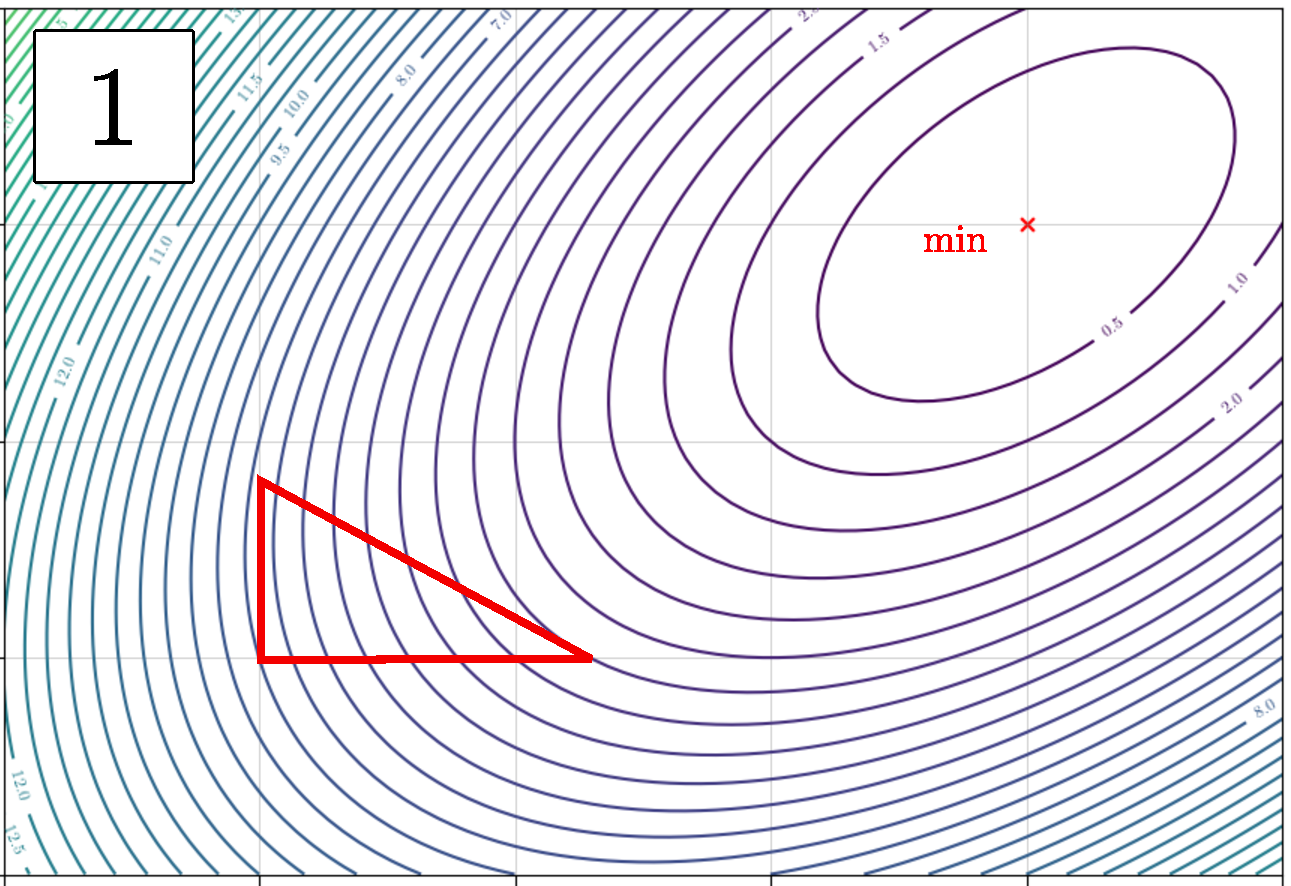
\includegraphics[width=0.96\textwidth, trim={0 0 0 0}, clip]{figures/nelder1.pdf}
	\end{subfigure}
	\begin{subfigure}[b]{0.325\textwidth}
		\centering
		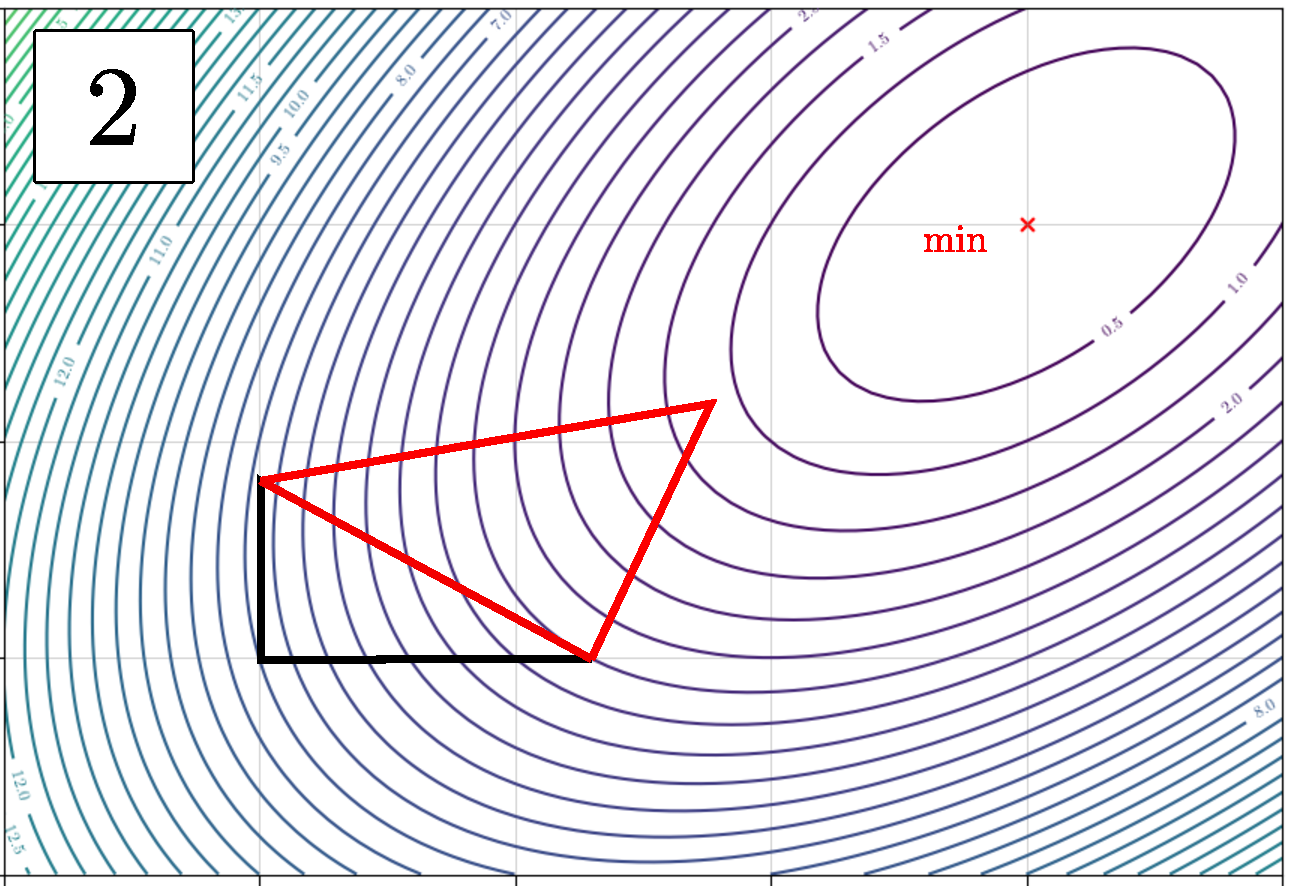
\includegraphics[width=0.96\textwidth, trim={0 0 0 0}]{figures/nelder2.pdf}
	\end{subfigure}
	\vspace{1mm}
	\begin{subfigure}[b]{0.325\textwidth}
		\centering
		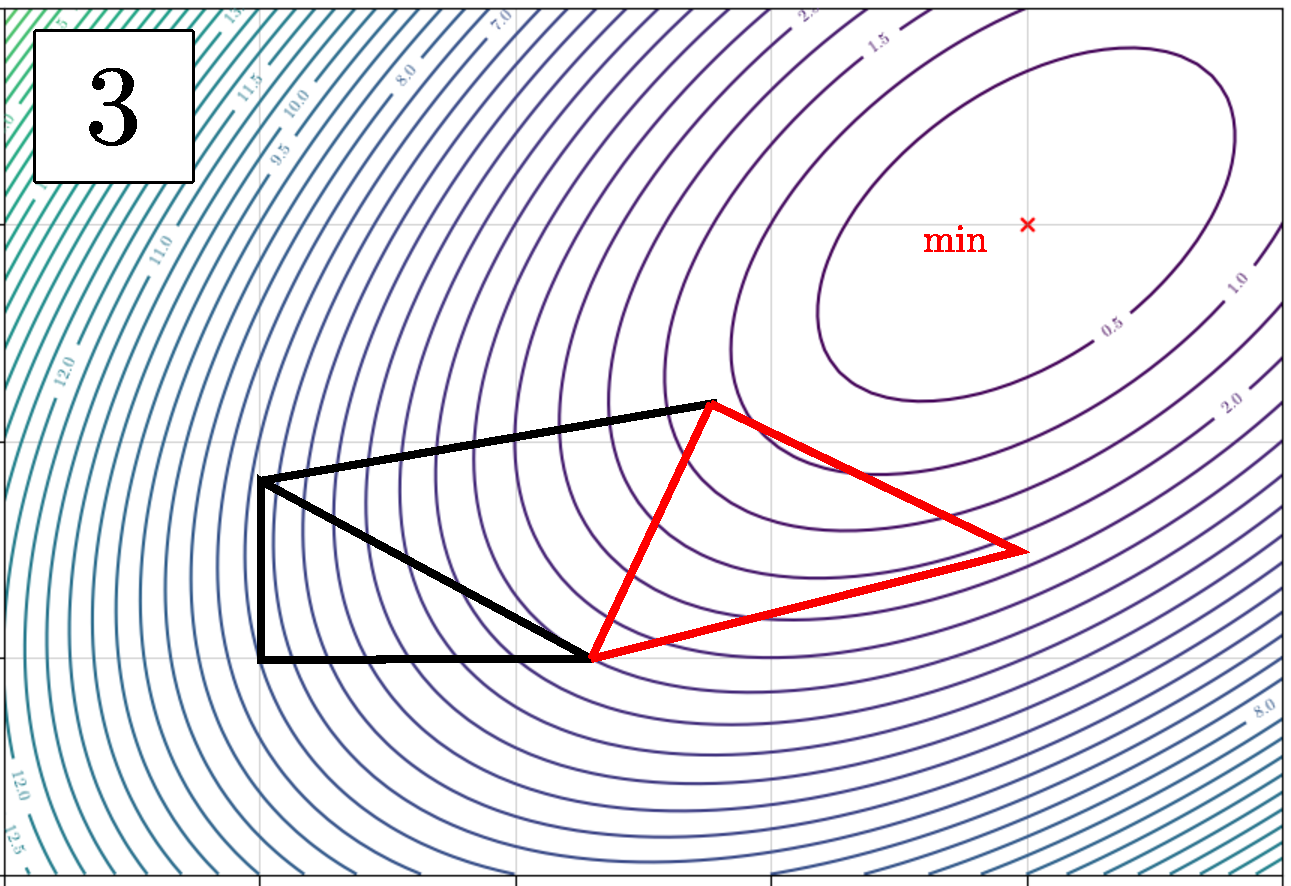
\includegraphics[width=0.96\textwidth, trim={0 0 0 0}]{figures/nelder3.pdf}
	\end{subfigure}
	\vspace{1mm}
	\begin{subfigure}[b]{0.325\textwidth}
		\centering
		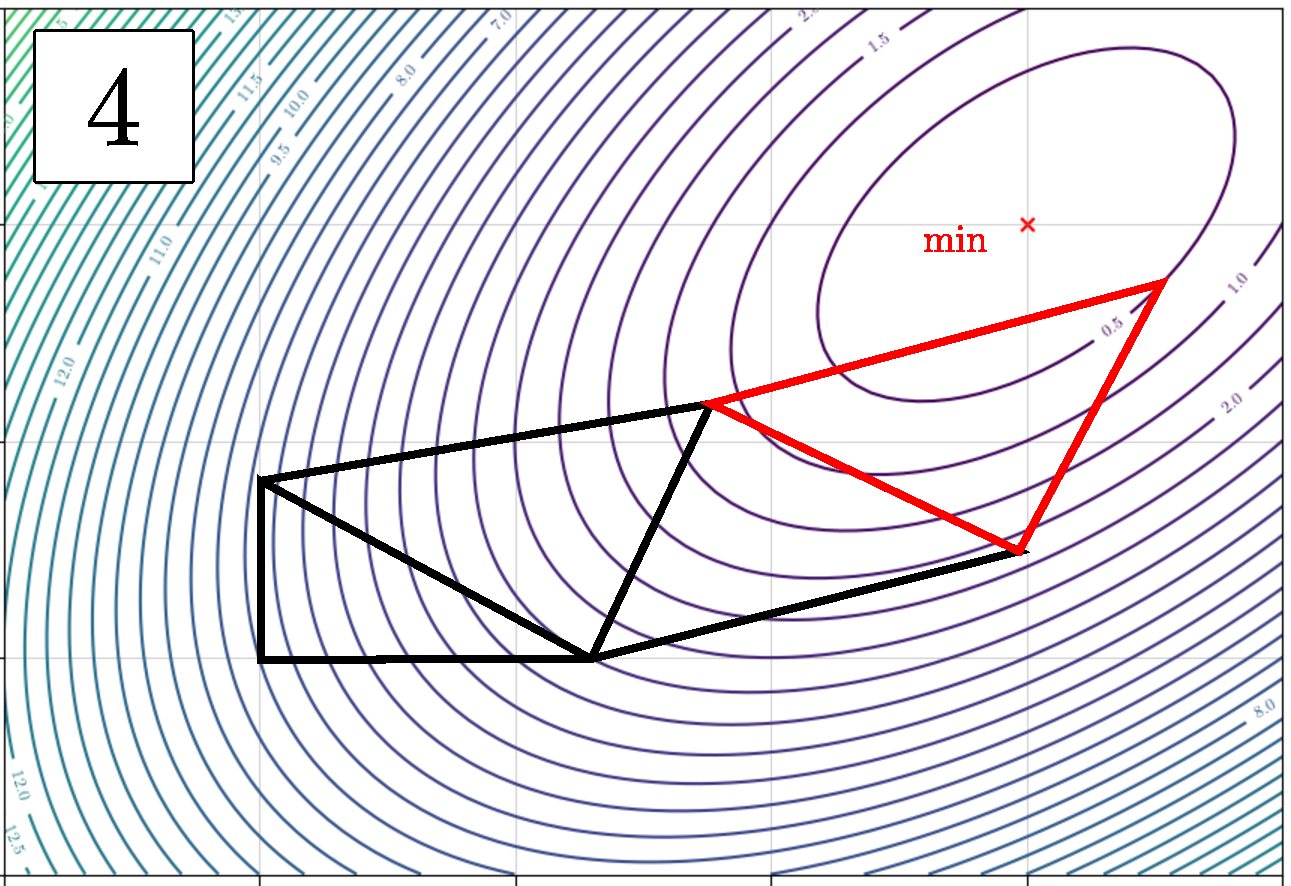
\includegraphics[width=0.96\textwidth, trim={0 0 0 0}]{figures/nelder4.pdf}
	\end{subfigure}
	\begin{subfigure}[b]{0.325\textwidth}
		\centering
		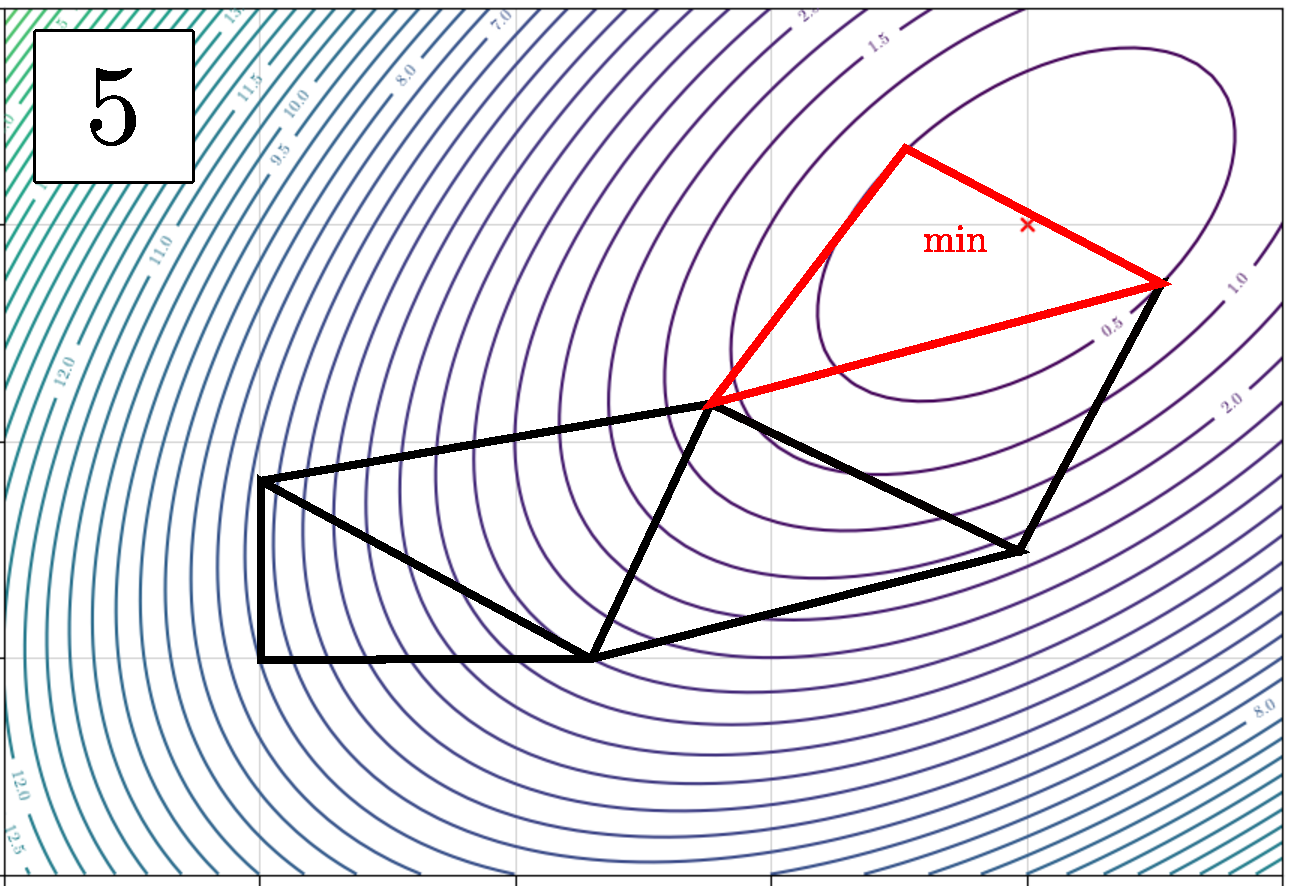
\includegraphics[width=0.96\textwidth, trim={0 0 0 0}]{figures/nelder5.pdf}
	\end{subfigure}
	\begin{subfigure}[b]{0.325\textwidth}
		\centering
		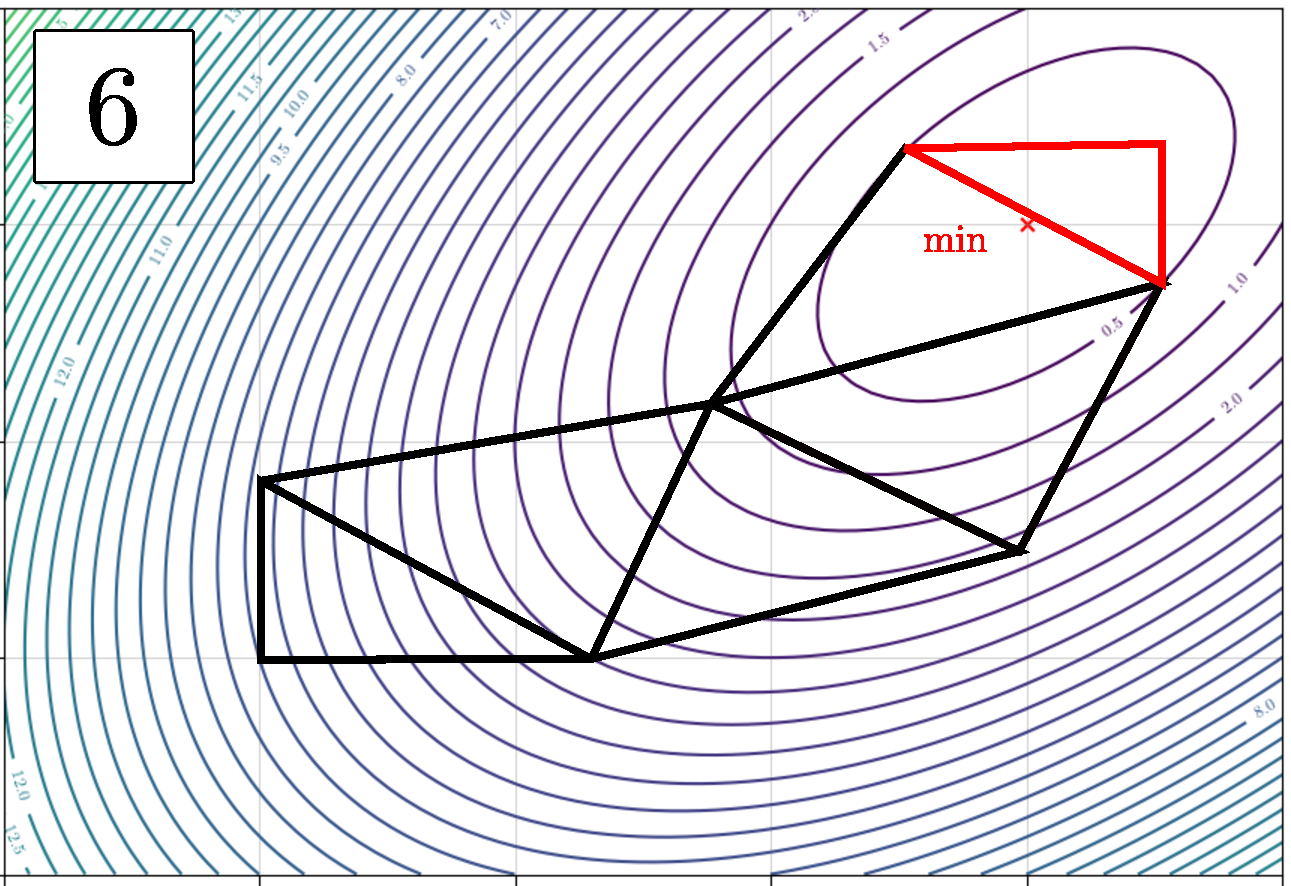
\includegraphics[width=0.96\textwidth, trim={0 0 0 0}]{figures/nelder6.pdf}
	\end{subfigure}
	\centering
	\begin{subfigure}[b]{0.325\textwidth}
		\centering
		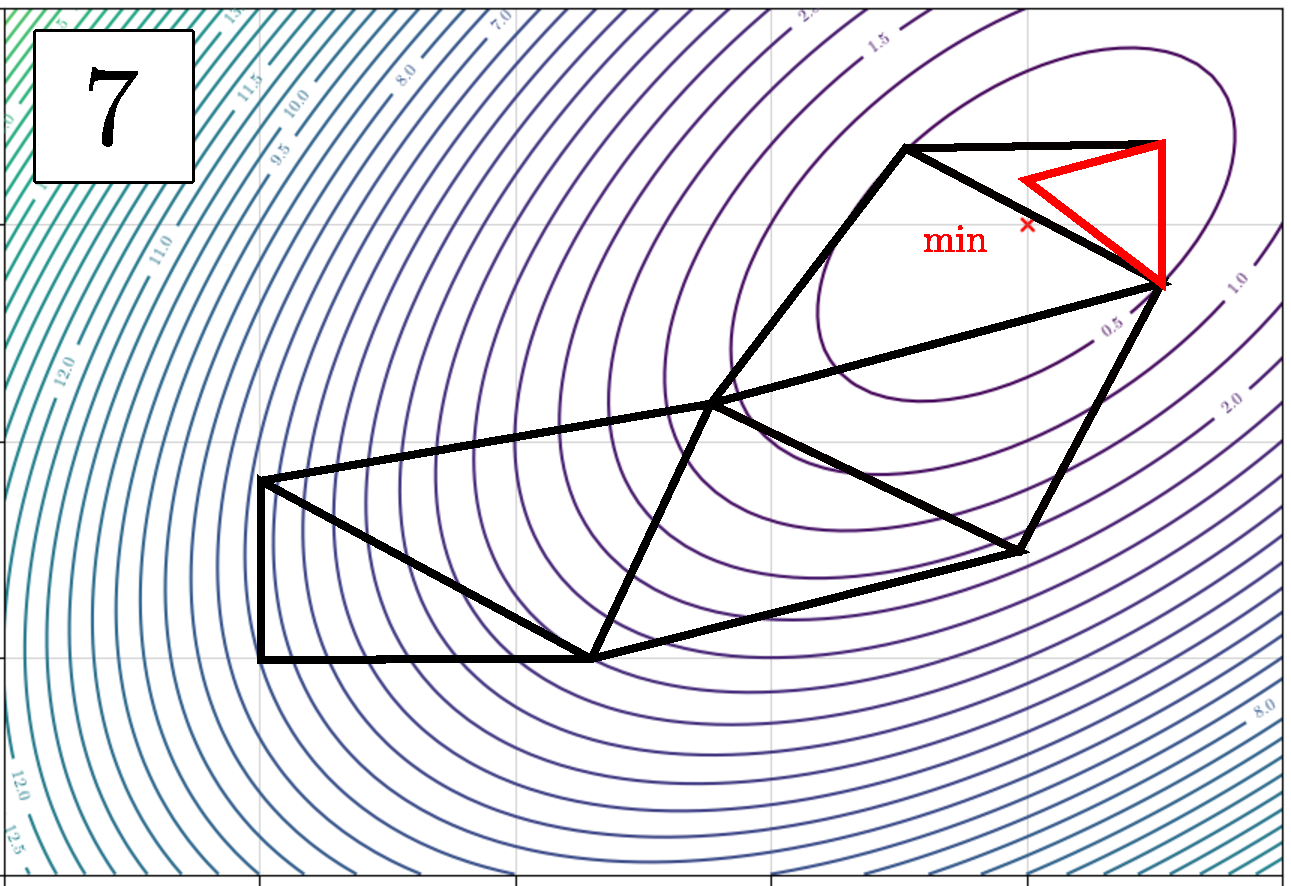
\includegraphics[width=0.96\textwidth, trim={0 0 0 0}]{figures/nelder7.pdf}
	\end{subfigure}
	\begin{subfigure}[b]{0.325\textwidth}
		\centering
		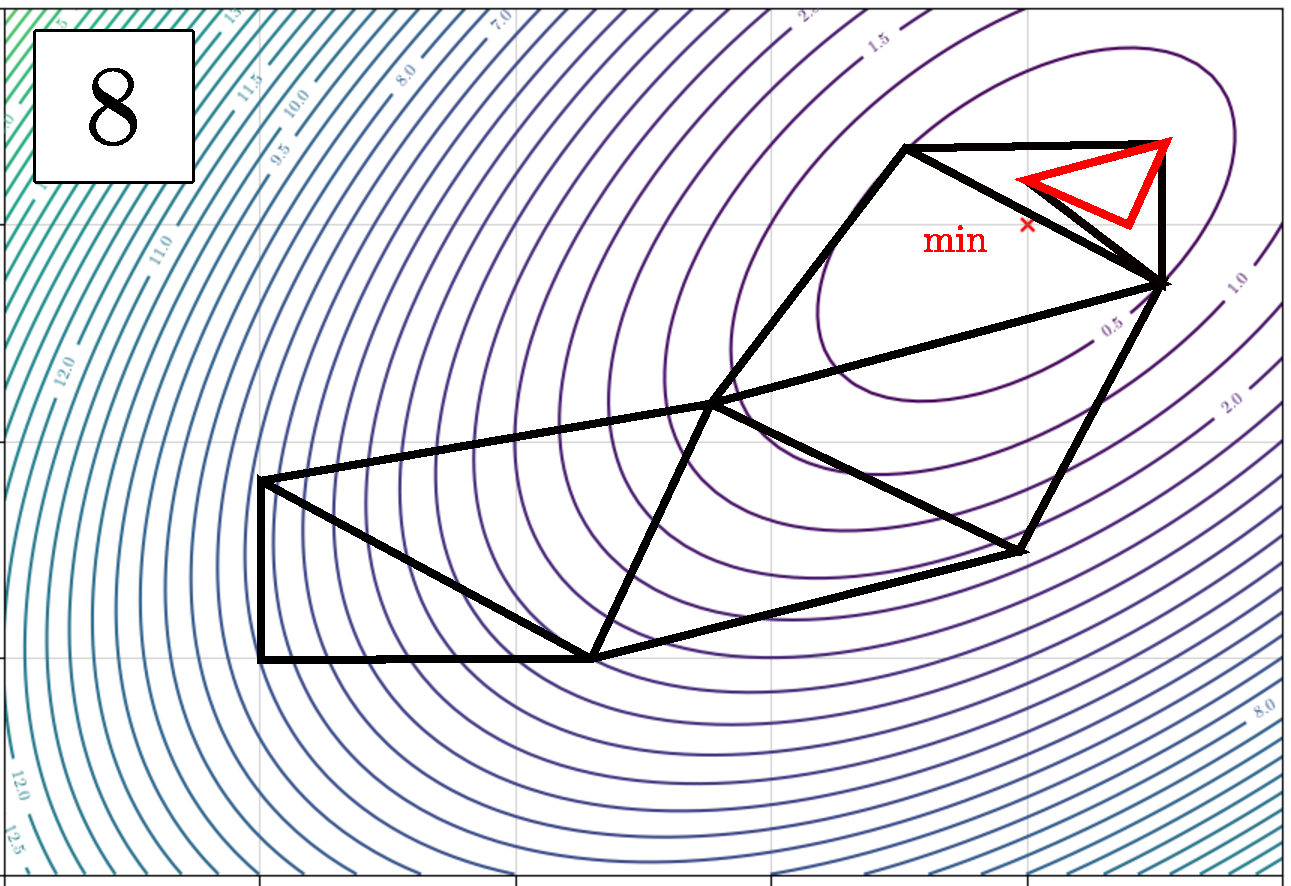
\includegraphics[width=0.96\textwidth, trim={0 0 0 0}]{figures/nelder8.pdf}
	\end{subfigure}
	\begin{subfigure}[b]{0.325\textwidth}
		\centering
		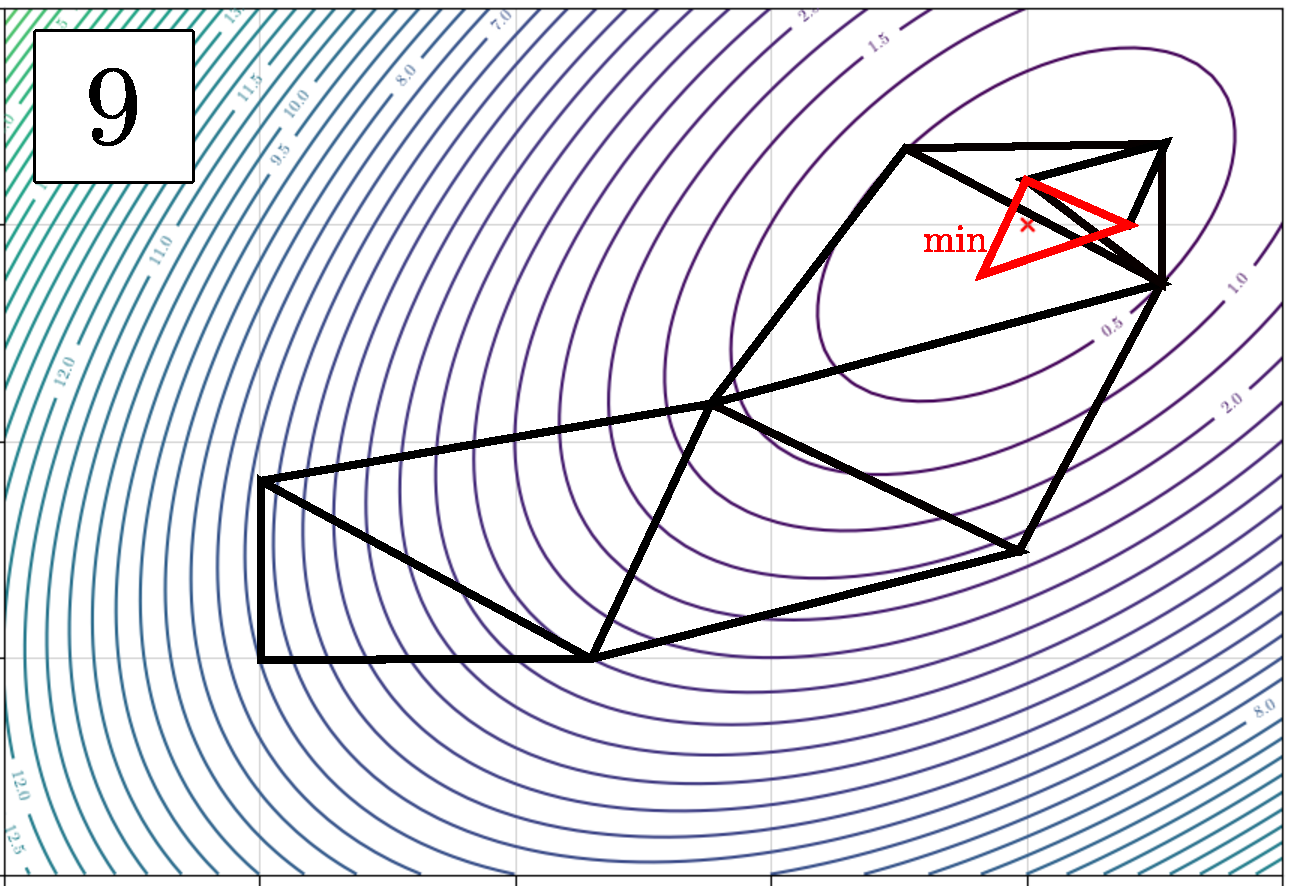
\includegraphics[width=0.96\textwidth, trim={0 0 0 0}]{figures/nelder9.pdf}
	\end{subfigure}
	\begin{center}
		\begin{subfigure}[b]{0.77\textwidth}
			\centering
			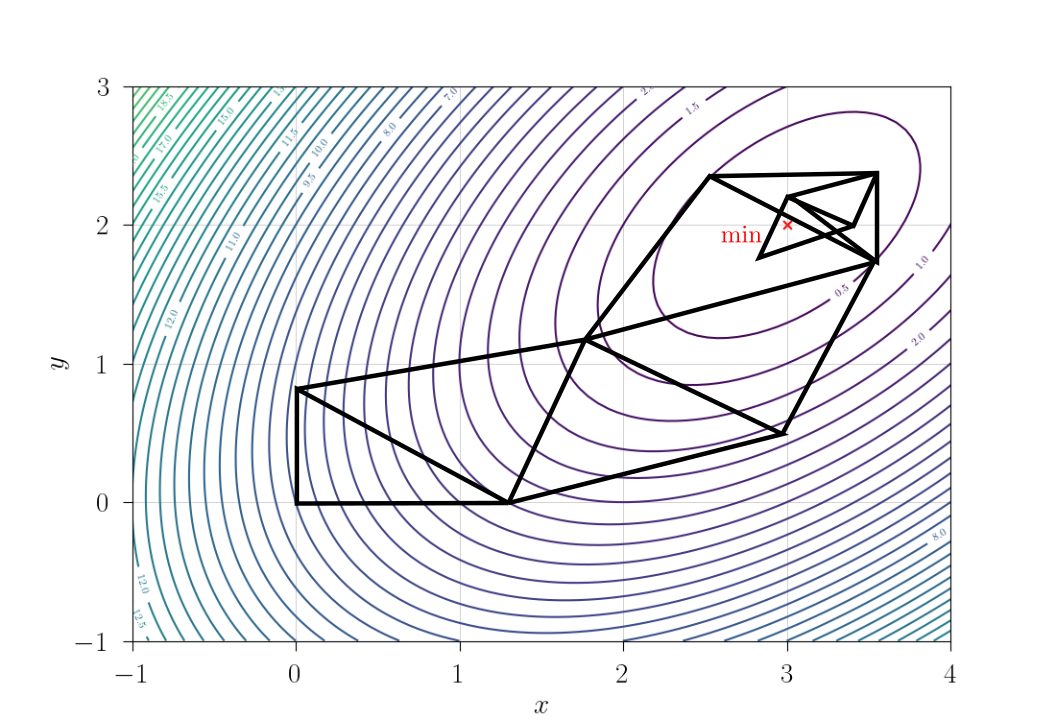
\includegraphics[width=0.985\textwidth, trim={0 6mm 0 7mm}]{figures/nelder.png}
		\end{subfigure}
	\end{center}
	
	\caption{Several iterations of the Nelder-Mead method for a specific choice of the initial simplex when minimizing the function $ x^2 - 4x + y^2 - y - xy + 7 $, with the minimum at the point (3,2) marked by a red cross.}
	\label{fig:NM}
\end{figure}


\subsection{Direct search methods}\label{direct-search}
In this part, we describe the \textit{generalized pattern search} (hereafter GPS) method \cite{Audet2002} and the \textit{mesh adaptive direct search} (hereafter MADS) method \cite{Audet2006}.

To describe the GPS algorithm, it is necessary to define a mesh, which is used to describe the search sets within the GPS algorithm. Let $ \mathbf{G} \in \mathbb{R}^{n \times n} $ be invertible and $ \mathbf{Z} \in \mathbb{Z}^{n \times p} $, $n, p \in \mathbb{N}$. Assume that every vector from $ \mathbb{R}^{n} $ can be expressed as a linear combination of the columns of matrix $ \mathbf{Z} $ (treated as vectors), such that all the coefficients in this linear combination are non-negative. Furthermore, let $ \mathbf{D} = \mathbf{G} \mathbf{Z} $. The mesh $ \mathbf{M} $ generated by $ \mathbf{D} $ centered at point $ \vec{x} $ is defined as
\begin{equation}
	\mathbf{M} = \left\{ \vec{x} + \delta \, \mathbf{D} y \, | \, y \in \mathbb{N}^p \right\},
\end{equation}
where $ \delta $ is called the mesh size parameter \cite{BBO-textbook, Audet2002}. In each iteration of the GPS algorithm, the shape of the mesh generally changes, as it is always centered at the point representing the best estimate in that iteration, and the size of the mesh step also changes. Let $ \vec{x}_k $ and $ \delta_k $ represent the estimate of the solution and the mesh size in the $ k $-th iteration, respectively. We 
then define the mesh in the $ k $-th iteration, denoted as $ \mathbf{M} _k $, as
\begin{equation}
	\mathbf{M} _k = \left\{ \vec{x}_k + \delta_k \, \mathbf{D} y \, | \, y \in \mathbb{N}^p \right\}.
\end{equation}
Note that the columns of matrix $ \mathbf{D} $, as defined above, can be interpreted as the possible directions in which the GPS algorithm searches the optimization space \cite{BBO-textbook, Audet2002}. Examples of search directions and meshes generated by different matrices $\mathbf{G}$ and $\mathbf{Z}$ are presented in Figure~\ref{fig:gps}.


\begin{figure}[H]
	\centering
	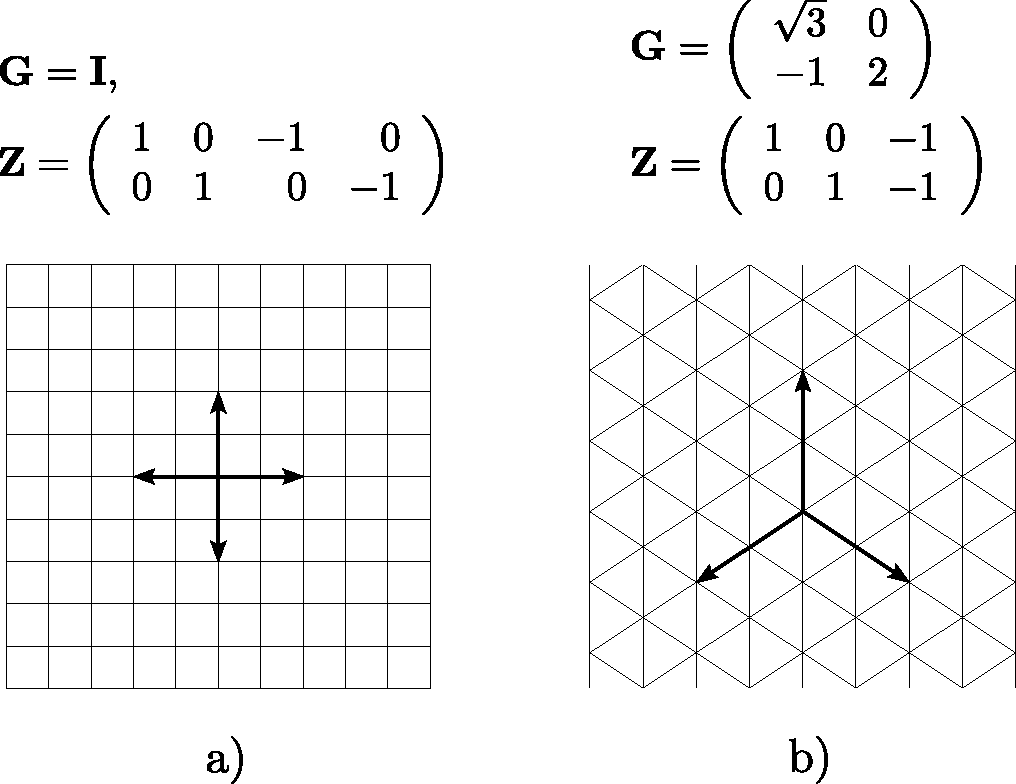
\includegraphics[width=0.70\textwidth]{figures/gps.pdf}
	\caption{Examples of search directions and meshes in $\mathbb{R}^2$ with
		obtained by different choices of $\mathbf{G}$ and~$\mathbf{Z}$. The mesh points
		are at the intersections of the lines, the arrows represent possible search directions.}
	\label{fig:gps}
\end{figure}


After initializing the necessary starting parameters, each iteration of the GPS algorithm is divided into two main steps. The first step is called the search step. During the search step, a finite set $S_k$ of candidate mesh points, selected according to a strategy specified by the user, is evaluated by computing the objective function at each one of the points. If none of the evaluated points represents an improvement over the value $ f(\vec{x}_k) $, the poll step follows. In the poll step, the objective function is evaluated at all neighboring mesh points of $ \vec{x}_k $. The poll set in $k$-th iteration is defined as $P_k = \{x_k + \delta_k d \, | \, d \in \mathbf{D}\}$. If none of the evaluated points represents an improvement over the value $ f(\vec{x}_k) $, we set $ \vec{x}_{k+1} = \vec{x}_k $ and decrease the mesh size, i.e., $ \delta_{k+1} < \delta_k $. However, if a point that improves the estimate of the solution is found in either the search or the poll step, this point is set as $ \vec{x}_{k+1} $, and the mesh size is increased, i.e., $ \delta_{k+1} > \delta_k $~\cite{BBO-textbook, Audet2002}.

The changes described above define a new mesh $ \mathbf{M} _k $ in each iteration. The mesh changes throughout the GPS algorithm. The algorithm terminates when $ \delta_{k+1} < \varepsilon $ for some user-specified $ \varepsilon > 0 $. It can be shown that the mesh step converges to zero, and under appropriate assumptions, the solution estimates converge to a stationary point of the objective function. Details can be found in \cite{BBO-textbook}. It should be noted that the convergence of GPS has been proven for unconstrained problems \cite{BBO-textbook}. The full GPS algorithm is presented in Algorithm~\ref{GPS-algo}.
\\[4pt]
\todo[inline]{Explain what is $t$ and $\tau$ in the algorithm, add typical ranges for $\tau$ maybe.}
\begin{algorithm}[H]
	\caption{Generalized Pattern Search (GPS) for unconstrained optimization}\label{GPS-algo}
	\begin{algorithmic}[1]
		\Require Function $f: \mathbb{R}^n \to \mathbb{R}$, initial point $x_0$, initial mesh size parameter $\delta_0$, positive spanning matrix $\mathbf{D}$, mesh size adjustment parameter $\tau \in (0, 1)$, stopping tolerance $\epsilon_{\text{stop}}$, iteration counter $k \gets 0$
		\Ensure Approximate optimal solution $\vec{x^{\star}}$ for function $f$
		
		\Procedure{GPS}{$x_0$}
		
		\While{$\delta_k > \epsilon_{\text{stop}}$}
		
		\Algphase{1. Search}
		\State Define a finite subset $S_k$ of the mesh $\mathbf{M}_k$
		\If{$f(t) < f(x_k)$ for some $t \in S_k$}
		\State Set $x_{k+1} \gets t$ and $\delta_{k+1} \gets \tau^{-1} \delta_k$
		\State \textbf{continue}
		\Else
		\State Go to Poll step
		\EndIf
		
		\Algphase{2. Poll}
		\State Select a positive spanning set $\mathbf{D}_k \subseteq \mathbf{D}$
		\State Define $P_k = \{x_k + \delta_k d : d \in \mathbf{D}_k\}$
		\If{$f(t) < f(x_k)$ for some $t \in P_k$}
		\State Set $x_{k+1} \gets t$ and $\delta_{k+1} \gets \tau^{-1} \delta_k$
		\Else
		\State $x_k$ is a mesh local optimizer
		\State Set $x_{k+1} \gets x_k$ and $\delta_{k+1} \gets \tau \delta_k$
		\EndIf
		
		\Algphase{3. Termination}
		\If{$\delta_{k+1} \leq \epsilon_{\text{stop}}$}
		\State \textbf{terminate}
		\Else
		\State Increment $k \gets k+1$ and continue
		\EndIf
		
		\EndWhile
		\EndProcedure
	\end{algorithmic}
\end{algorithm}

We turn our attention to the MADS algorithm, which generalizes the GPS algorithm by allowing for a different set of polling directions. The key difference is that MADS introduces the concept of a frame, which allows the poll directions to form a dense subset in $ \mathbb{R}^{n} $ as the algorithm progresses~\cite{BBO-textbook, derivative-free-review}. The frame $\mathbf{F}_k$ at iteration $k$ is defined as
\begin{equation}
	\mathbf{F}_k = \{ \vec{x} \in \mathbf{M}_k \ \big| \ \| \vec{x} - \vec{x}_k \|_\infty \leq \Delta_k b \},
\end{equation}
where $M_k$ represents the current mesh, $ \Delta_k $ is the frame size parameter, satisfying $ \delta_k \leq \Delta_k $, and $b = \max \ \{ \| d \| _\infty \ \big| \ d \in \mathbf{D} \}$. The extent of the frame is determined by the parameter $ \Delta_k $, and the polling directions are taken from this frame.

Each iteration of the MADS algorithm begins similarly to GPS, with a search step where a finite set $S_k$ of candidate points, selected based on the current mesh, is evaluated by computing the objective function at each of the points. If none of these points improves upon the current best solution, the algorithm proceeds to the poll step. 
 
The poll set $P_k$ is a subset of points selected from $\mathbf{F}_k$ and $\mathbf{M}_k$. Trivially, $P_k \subseteq \mathbf{F}_k \subseteq \mathbf{M}_k$. Importantly, the mesh size parameter $ \delta_k $ is allowed to decrease more rapidly than the  enabling the poll directions to asymptotically become arbitrarily dense~\cite{Audet2006}. This aspect is crucial, as it ensures that MADS can explore directions in a finer and more systematic manner than GPS, leading to better convergence properties.


\begin{figure}[H]
	\centering
	\vspace{0.5cm}
	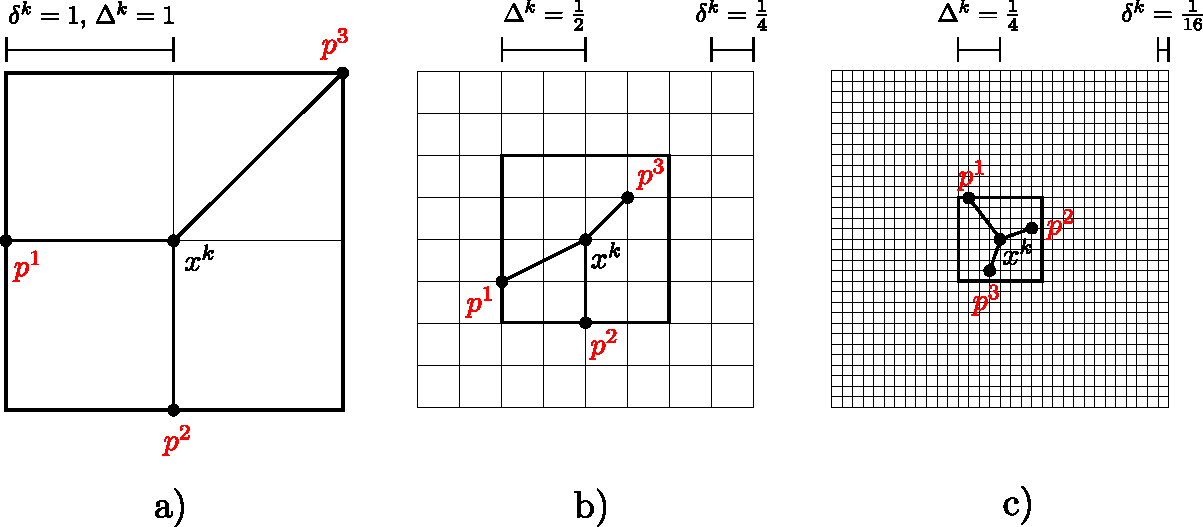
\includegraphics[width=1.01\textwidth]{figures/mads.pdf}
	\caption{Examples of meshes and frames $\mathbb{R}^2$ for different
		values of $\delta_k$ and $\Delta_k$}
	\label{fig:mads}
\end{figure}

If an improvement is found in the poll step, the new point is set as $ \vec{x}_{k+1} $, and the frame size $ \Delta_k $ and mesh size $ \delta_k $ may be increased to encourage further exploration. Conversely, if no improvement is found, $ \vec{x}_{k+1} = \vec{x}_k $, and the mesh size is reduced, i.e., $ \delta_{k+1} < \delta_k $, to allow for a more local search. The process of shrinking and refining the frame and mesh sizes continues until $ \delta_k $ falls below a user-specified threshold, at which point the algorithm terminates.

MADS also incorporates the \textit{extreme barrier function} to handle constraints, similarly to GPS. For constrained optimization problems, the objective function is modified into an extreme barrier function~\cite{BBO-textbook}, which penalizes any infeasible points by assigning them an infinite objective value. This simple yet effective strategy ensures that the optimization remains focused on feasible regions of the search space, and the algorithm converges to a stationary point even for constrained problems. A full description of the MADS algorithm and its implementation details can be found in~\cite{BBO-textbook}.



\begin{algorithm}[H]
	\caption{Mesh Adaptive Direct Search (MADS) for constrained optimization}\label{MADS}
	\begin{algorithmic}[1]
		\Require Function $f_{\infty}: \mathbb{R}^n \to \mathbb{R} \cup \{\infty\}$, initial point, initial frame size parameter $\Delta_0$, positive spanning matrix $\mathbf{D}$, mesh size adjustment parameter $\tau \in (0,1)$, stopping tolerance $\epsilon_{\text{stop}}$, iteration counter $k \gets 0$
		\Ensure Approximate optimal solution $\vec{x^{\star}}$ for function $f$
		
		\Procedure{MADS}{$x_0$}
		
		\While{$\Delta_k > \epsilon_{\text{stop}}$}
		
		\Algphase{1. Parameter Update}
		\State Set the mesh size parameter $\delta_k = \min \{\Delta_k, (\Delta_k)^2\}$
		
		\Algphase{2. Search}
		\State Define a finite set $S_k \subset \mathbf{M}_k$ such that:
		\If{$f_{\infty}(t) < f_{\infty}(x_k)$ for some $t \in S_k$}
		\State Set $x_{k+1} \gets t$ and $\Delta_{k+1} \gets \tau^{-1}\Delta_k$
		\State \textbf{continue}
		\Else
		\State Go to Poll step
		\EndIf
		
		\Algphase{3. Poll}
		\State Select a positive spanning set $\mathbf{D}_{k}$ and define:
		\State $P_k = \{x_k + \delta_k d : d \in \mathbf{D}_{k}\}$, a subset of the frame $\mathbf{F}_k$ with extent $\Delta_k$
		\If{$f_{\infty}(t) < f_{\infty}(x_k)$ for some $t \in P_k$}
		\State Set $x_{k+1} \gets t$ and $\Delta_{k+1} \gets \tau^{-1}\Delta_k$
		\Else
		\State Set $x_{k+1} \gets x_k$ and $\Delta_{k+1} \gets \tau\Delta_k$
		\EndIf
		
		\Algphase{4. Termination}
		\If{$\Delta_{k+1} \leq \epsilon_{\text{stop}}$}
		\State \textbf{terminate}
		\Else
		\State Increment $k \gets k+1$ and continue
		\EndIf
		
		\EndWhile
		\EndProcedure
	\end{algorithmic}
\end{algorithm}
\subsection{Optimization Using a Surrogate Model}\label{model-based}
In cases where evaluating the objective function at a specific point is time-consuming or computationally expensive, it can be useful to employ a surrogate model for the objective function during optimization. We define a surrogate model of the given problem as the problem

\begin{equation}
	\min_{\vec{x} \in \mathbf{\tilde{X}}} \tilde{f}(\vec{x}),
\end{equation}
where
\begin{equation}
	\mathbf{\tilde{X}} = \left\{ \vec{x} \in \mathbf{D} \subseteq \mathbb{R}^n \ \middle| \ \vec{\tilde{g}} (\vec{x}) \leq \vec{0} \wedge \vec{\tilde{h}} (\vec{x}) = \vec{0} \right\},
\end{equation}
and the functions \( \tilde{f}, \vec{\tilde{g}} \), and \( \vec{\tilde{h}} \) have characteristics similar to those of the functions \( f, \vec{g} \), and \( \vec{h} \) in the original problem. The characteristics of \( \tilde{f}, \vec{\tilde{g}} \), and \( \vec{\tilde{h}} \) are intentionally left undefined, reflecting the fact that the surrogate model does not necessarily need to be an accurate approximation of the original problem \cite{BBO-textbook, two-decades, Kramer2011}. A good approximative model may not always be a suitable surrogate for optimization purposes, a situation illustrated in Figure \ref{fig:surrogate}.

\begin{figure}[H]
	\centering
	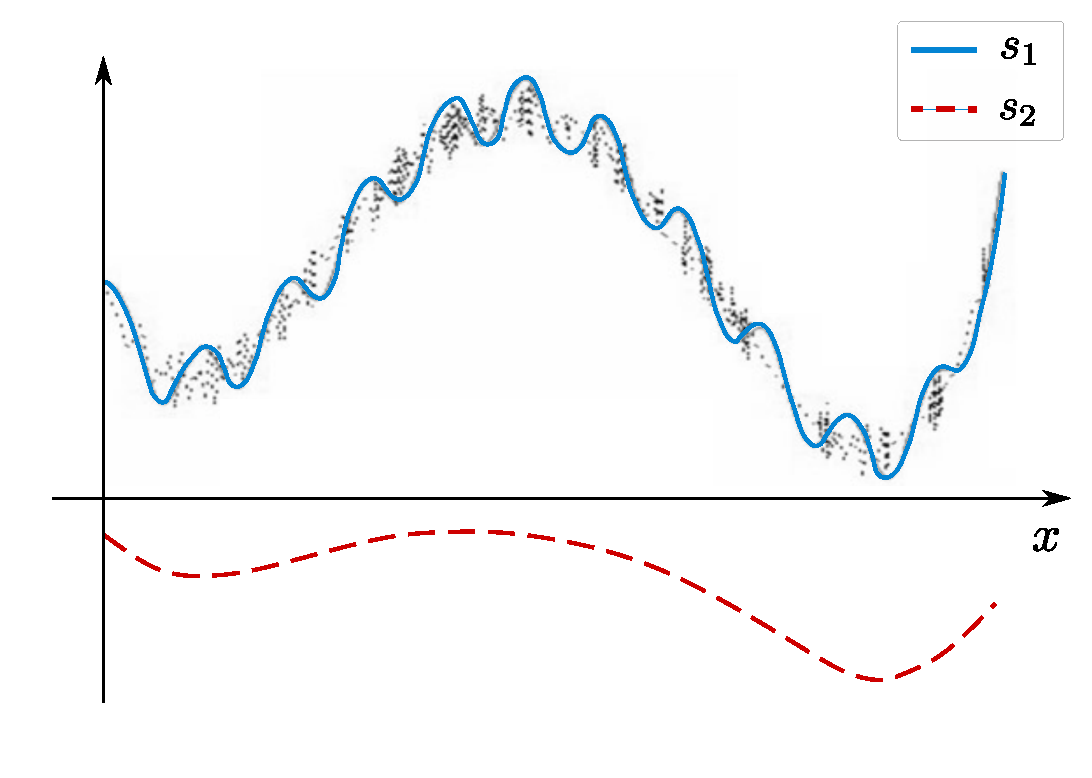
\includegraphics[width=0.6\textwidth]{figures/surrogate.pdf}
	\caption{An illustration of two surrogate models, $ s_1 $ and $ s_2 $. The black points represent noisy values of the objective function. While using surrogate model $ s_1 $ represents a better choice for approximating the function, it is not suitable for optimization since $ s_1 $ contains many undesirable stationary points that the original objective function does not have. On the other hand, while surrogate model $ s_2 $ is not as accurate in approximating the function's values, it is a better choice for optimization because the stationary points of $ s_2 $ are almost identical to those of the optimized objective function.}
	\label{fig:surrogate}
\end{figure}

Using a surrogate model in optimization is often just a part of a more complex optimization method. Surrogate models can, for example, be used within GPS and MADS methods described in section \ref{direct-search}, where, during the poll step, we first evaluate the surrogate function \( \tilde{f} \) at the points from the poll set, sort these values, and use them to sort the poll set used to evaluate the original function \( f \). This potentially allows us to significantly reduce the time required to complete the poll step, as sorting the points increases the probability of finding a better estimate of the solution at one of the first examined points \cite{BBO-textbook}. Surrogate models can also be used within other methods to accelerate the optimization process, and their application is discussed in detail in \cite{BBO-textbook, two-decades}.

%\section{Description of the optimization framework}\label{framework}
A fully automated and modular optimization framework was developed to solve the optimization problems in this work. The proposed framework is composed of several components, which are described in detail below:

\begin{enumerate}
	\item \textbf{Optimization}:  
	The first component encompasses the optimization method, which governs the entire process. In this part, the optimization problem is defined along with any required constraints.
	
	In this study, we use the Nelder-Mead method, implemented in Python specifically for this work and detailed in Appendix~\ref{appendix B}. Additionally, the framework includes the MADS method (see Section~\ref{direct-search}), implemented in the open-source \texttt{NOMAD} library \cite{nomad} in C++. For handling constraints in both the Nelder-Mead and MADS methods, we use the extreme barrier function.
	
	\item \textbf{Geometry Generation}:  
	The optimization parameters, updated at each iteration, are passed to the geometry generator. For generating the geometries used in numerical simulations, we use the \texttt{meshgen} package detailed in Chapter~\ref{geometry}.
	
	\item \textbf{Numerical Simulation}:  
	The final component of the optimization framework is the numerical solver, which evaluates the objective function based on the generated geometry. Numerical simulations are performed using the LBM, which is described alongside additional implementation details in Chapter~\ref{lbm}.
\end{enumerate}

The interconnection of these components within the optimization framework is schematically illustrated in Figure~\ref{fig:framework}.


\begin{figure}[H]
	\vspace{5mm}
	\centering
	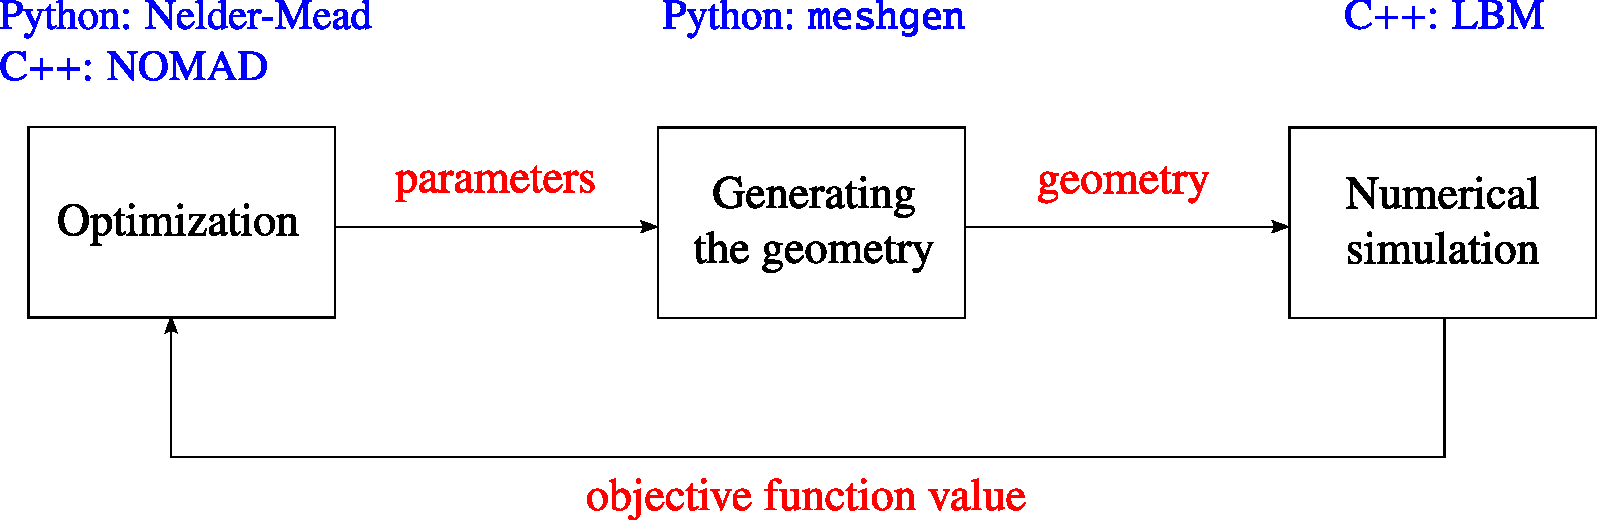
\includegraphics[width=0.95\textwidth]{figures/framework-en.pdf}
	\vspace{5mm}
	\caption{Schematic representation of the modular optimization framework. It consists of three main components: (1) Optimization, which defines the problem and governs the iterative process, (2) Geometry generation, where optimization parameters are translated into geometric models using \texttt{meshgen}, and (3) Numerical simulation, where the objective function is evaluated using the LBM.}
	\label{fig:framework}
	
\end{figure}

Mathematical optimization, also known as mathematical programming,  is a broad field that covers wide range of methods and problem types, including linear and nonlinear optimization, convex programming, and integer programming \cite{Kochenderfer2019}. Selecting an appropriate optimization method for a given problem is a crucial step, as factors such as nonlinearity, the presence of constraints, and the computational cost of evaluating the objective function can significantly influence performance. In many cases, classic gradient-based algorithms—such as the Davidon-Fletcher-Powell \cite{Fletcher1963} or Broyden-Fletcher-Goldfarb-Shanno \cite{broyden1970} methods—can be applied efficiently. However, these methods become less practical when gradients are difficult to obtain analytically and must instead be computed numerically. Numerical gradient estimation can be slow, computationally expensive, and prone to inaccuracies.

In this work, we solve a constrained, nonlinear optimization problem in which the objective function is computed numerically and may take several hours per evaluation. Previous studies \cite{buresBP, buresVU} examined the coupling of various optimization algorithms, including gradient-based methods, with the numerical simulations underlying our objective function. Those studies showed that gradient-based approaches are not well-suited to our current black-box setting. In contrast, gradient-free methods avoid the costs and complexities of gradient approximation, providing a more suitable option in such settings. This naturally guides us toward employing gradient-free optimization methods in this work.

When dealing with constraints, standard approaches such as penalty and barrier methods offer systematic ways to ensure feasibility \cite{Bert}. However, they often require multiple runs of a modified, unconstrained subproblem \cite{Bert}, which can become prohibitively time-consuming in our context. That is why we adopt a simplified approach to constraint handling known as the extreme barrier function \cite{BBO-textbook}, which allows us to incorporate constraints directly without extensive computational costs.

This chapter is structured as follows: First, we formally define the general optimization problem under consideration. Next, we discuss black-box optimization methods and their relevance to our scenario. Finally, we present the proposed optimization framework in detail, highlighting its components and illustrating how they are interconnected.

\section{General optimization problem}

Let $m, n, q \in \mathbb{N}$. Define the continuous functions $f : \mathbf{D} \rightarrow \mathbb{R}$, $ \vec{g} : \mathbf{D} \rightarrow \mathbb{R}^m$, $ \vec{h} : \mathbf{D} \rightarrow \mathbb{R}^q $, where $ \mathbf{D} = \mathrm{Dom} \, (f) \cap \mathrm{Dom} \, (\vec{g}) \cap \mathrm{Dom} \, (\vec{h})$, i.e., $ \mathbf{D} $ is the intersection of the domains of the given functions. Next, define the set

\begin{equation}\label{eq:feasible solution}
	\mathbf{X} = \big\{ \vec{x} \in \mathbf{D} \subseteq \mathbb{R}^n \ | \ \vec{g} (\vec{x}) \leq \vec{0} \wedge \vec{h} (\vec{x}) = \vec{0} \, \big\},
\end{equation}
where the inequality $ \vec{g} \leq \vec{0} $ and equality $ \vec{h} = \vec{0} $ are understood component-wise. The general goal of mathematical optimization is to solve the problem
\begin{equation}\label{eq:basic problem}
	\min_{\vec{x} \in \mathbf{X}} f(\vec{x}).
\end{equation}

The function $f$ being minimized is called the objective function, $\mathbf{D}$ is referred to as the domain of the problem, and $\mathbf{X}$~is called the set of feasible solutions of the problem \cite{Bert}. Note that, henceforth, $f$ denotes only the objective function and not the distribution function discussed in Chapter \ref{lbm}.

When classifying optimization problems, we refer to what are known as constraints. These are determined by the definition of the set $ \mathbf{X} $, i.e., the equality and inequality conditions for the functions $ \vec{g} $~and $ \vec{h} $, and by the domain $ \mathbf{D} $. Constraints defined by $ \vec{g} (\vec{x}) \leq \vec{0} \wedge \vec{h} (\vec{x}) = \vec{0} $ are called explicit constraints, while those determined by the domain $ \mathbf{D} $ are called implicit constraints.
\newpage
The optimal solution of the problem \eqref{eq:basic problem} is denoted by $ \vec{x}^{\star} \in \mathbf{X} $ and is defined as
\begin{equation}
	\vec{x}^{\star} = \operatorname*{argmin}_{\vec{x} \in \mathbf{X}} \, f(\vec{x}).
\end{equation}
Note that the optimal solution may not be unique, and we refer to the set of all optimal solutions as the optimal set. It is also important to recognize that the search for an optimal solution can equivalently be formulated as finding the maximum of the function $ -f$ over the same set $ \mathbf{X}$, enabling the use of the same techniques for solving maximization problems \cite{Bert, non-linear-textbook}.
\section{Black-box optimization}\label{black-box}
In practice, we often need to optimize an objective function $f$ whose exact form and derivative are unknown. This is common in numerical simulations, where the function can only be evaluated at specific points. Moreover, evaluating the function at a point may be difficult, time-consuming, or computationally expensive. As a result, standard optimization algorithms are not well-suited for these problems.

The discipline that deals with problems where the objective function (or constraints) is given by a so-called black-box\footnote{In programming, a black-box refers to a system whose internal mechanisms are unknown to the user. This means that the user generally has access only to the system’s input and output \cite{BBO-textbook}.}, is called black-box optimization (hereafter referred to as BBO). In BBO, it is typically not assumed that the objective function is continuous or differentiable \cite{BBO-textbook, derivative-free-review, two-decades}.

It is worth noting that in the literature, black-box optimization is often confused with derivative-free optimization (DFO), which encompasses methods and techniques for objective functions whose derivatives are unknown or difficult to compute \cite{BBO-textbook, derivative-free-review, Kramer2011}. These two disciplines share many common characteristics, but they differ primarily in that, within DFO, the formula for calculating the derivative of the objective function may still be known. Furthermore, BBO includes heuristic methods, whereas DFO focuses mainly on methods that can be reliably analyzed mathematically in terms of convergence and stopping criteria, which is often not possible for BBO methods \cite{BBO-textbook}. Therefore, although the terms BBO and DFO are often used interchangeably, in this work, we will treat them as two distinct disciplines \cite{BBO-textbook}.

Additionally, it should be noted that various classifications of methods within BBO can be found in the literature. In this work, we will adhere to the classification presented in \cite{BBO-textbook}, distinguishing between heuristic methods, direct search methods, and methods based on surrogate models. Each of these classes will be briefly described in this section.


\subsection{Heuristic Methods}\label{heuristic}
Heuristic optimization methods often rely on different predefined rules or even trial and error when seeking the solution of an optimization problem. These methods usually do not guarantee optimal solutions, but they are often effective for finding near-optimal results in a reasonable amount of time. Heuristic methods include genetic algorithms, detailed in \cite{BBO-textbook}, along with various other heuristic approaches.

In this section, however, we will focus on a different widely used heuristic method, the Nelder-Mead method, also known as the simplex method\footnote{A simplex in $ \mathbb{R}^n $ is defined as a bounded convex polytope (a generalization of a polyhedron to any dimension) with a non-empty interior and exactly $ n+1 $ vertices \cite{BBO-textbook}.}\footnote{The term "simplex method" more commonly refers to the algorithm used to find the optimal solution in linear programming. This algorithm was developed by George Dantzig \cite{Dantzig1990}.}\cite{Nelder1965}.

The Nelder-Mead method finds a solution to an optimization problem by iteratively constructing simplexes. The process begins by initializing a starting simplex. The objective function is then evaluated at each vertex of this simplex. In each subsequent iteration, the simplex is transformed in order to move closer to the position of the sought stationary point of the objective function. The transformation of the simplex involves manipulating its points using predefined operations -- expansion, reflection, contraction (inner and outer), and shrinking, which are schematically illustrated in Figure~\ref{fig:NM operations}. 

\begin{figure}[H]
	%	\vspace{5mm}
	\centering
	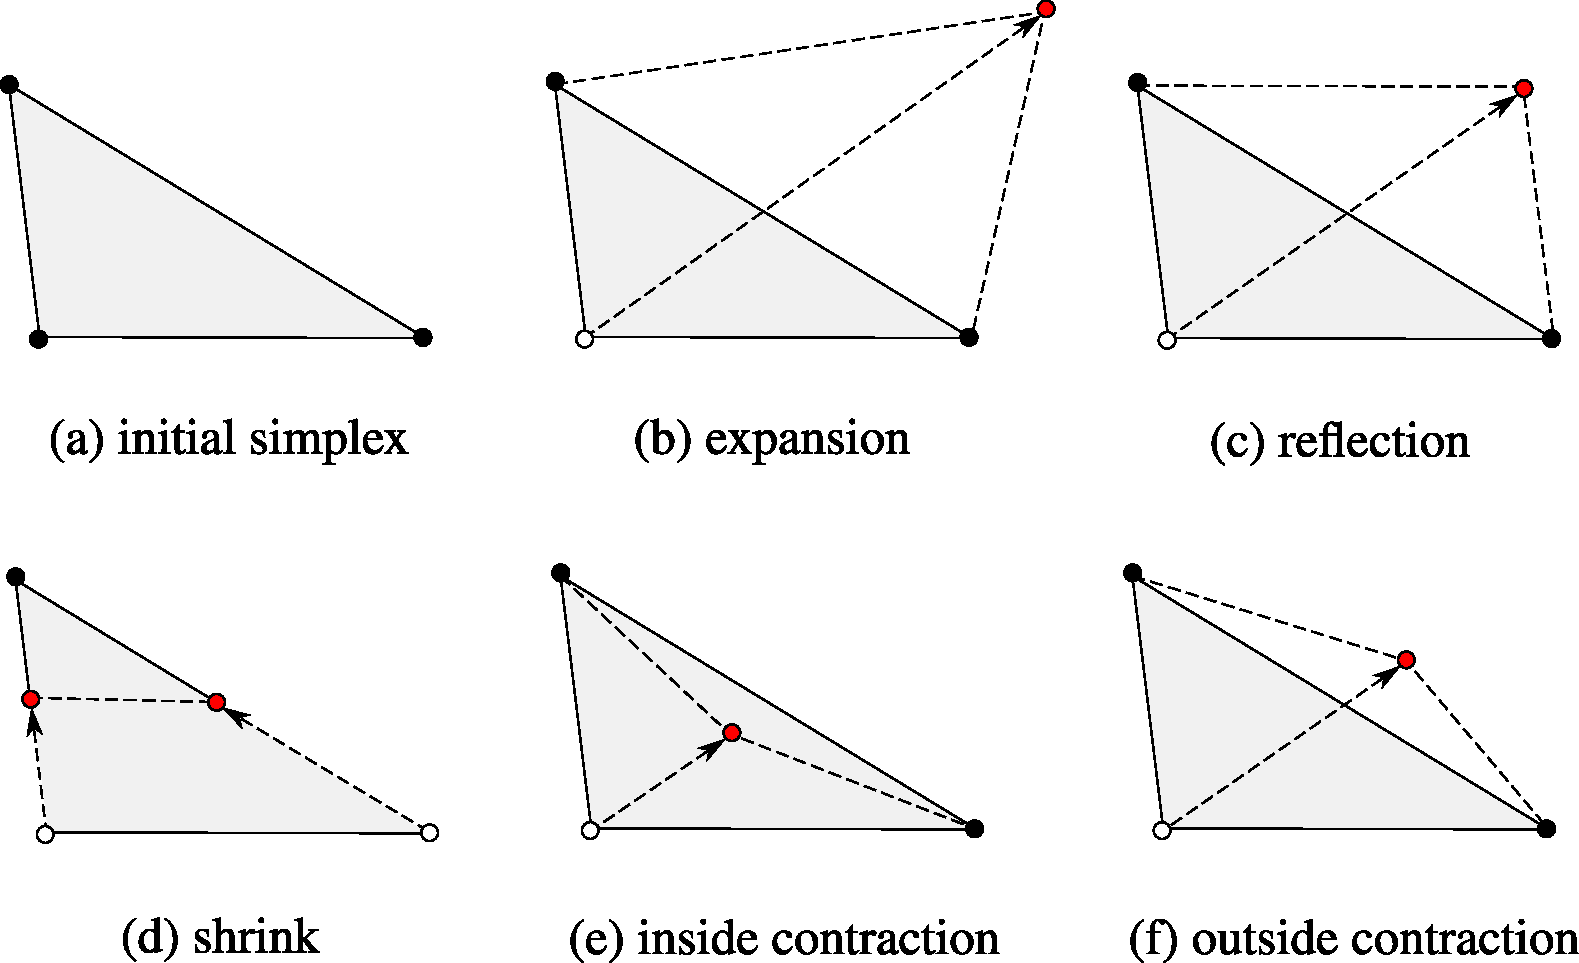
\includegraphics[width=0.96\textwidth]{figures/neldermead.pdf}
	\vspace{2mm}
	\caption{A schematic representation of the operations used to transform simplexes in the Nelder-Mead method. The vertices generated by applying each operation are shown in red. For clarity, the operations are depicted in $ \mathbb{R}^2 $.}
	%	\vspace{2mm}
	\label{fig:NM operations}
\end{figure}

The transformations performed during each iteration are determined by comparing the function values at the vertices of the simplex. The newly formed simplex shares either exactly one vertex or exactly $ n $ vertices with the simplex from the preceding iteration. The algorithm continues to iteratively transform the simplex until a stopping condition (specified by the user) is met \cite{BBO-textbook}. Details of the Nelder-Mead method, including the algorithm's description and the choice of stopping condition, are discussed in \cite{BBO-textbook, derivative-free-review, Nelder1965}. The full Nelder-Mead method algorithm is presented in Algorithm~\ref{neldermead}.

\begin{algorithm}
	\caption{Nelder-Mead algorithm}\label{neldermead}
	\begin{algorithmic}[1]
		\Require Initial simplex $S^0 = \{s^0, s^1, \dots, s^n\}$, function $f: \mathbb{R}^n \to \mathbb{R}$, parameters $\delta^{\text{e}}$, $\delta^{\text{oc}}$, $\delta^{\text{ic}}$, $\gamma$, iteration counter $k \gets 0$
		\Ensure Approximate optimal solution $\vec{x^{\star}}$ for function $f$
		
		\Procedure{Nelder-Mead}{$S^0$}
		\State Reorder $S^k$ so that $f(s^0) \leq f(s^1) \leq \dots \leq f(s^n)$
		\State Set $f^k_{\text{best}} = f(s^0)$
		
		\While{stopping condition not met}
		\Algphase{Reflection}
		\State Compute centroid $x^{\text{c}} = \frac{1}{n} \sum_{i=0}^{n-1} s^i$
		\State Set reflection point $x^{\text{r}} = x^{\text{c}} + (x^{\text{c}} - s^n)$ and compute $f^{\text{r}} = f(x^{\text{r}})$
		\If{$f^k_{\text{best}} \leq f^{\text{r}} < f(s^{n-1})$}
		\State Set $S^{k+1} = \{s^0, s^1, \dots, s^{n-1}, x^{\text{r}}\}$
		\State Increment $k \gets k+1$ and continue
		\EndIf
		
		\Algphase{Expansion}
		\If{$f^{\text{r}} < f^k_{\text{best}}$}
		\State Set expansion point $x^{\text{e}} = x^{\text{c}} + \delta^{\text{e}} (x^{\text{r}} - x^{\text{c}})$ and compute $f^{\text{e}} = f(x^{\text{e}})$
		\If{$f^e < f^r$}
		\State Set $S^{k+1} = \{s^0, s^1, \dots, s^{n-1}, x^\text{e}\}$
		\Else
		\State Set $S^{k+1} = \{s^0, s^1, \dots, s^{n-1}, x^\text{r}\}$
		\EndIf
		\State Increment $k \gets k+1$ and continue
		\EndIf
		
		\Algphase{Contraction}
		\If{$f^\text{r} \geq f(s^n)$}
		\State \textbf{Outside Contraction:} Compute $x^\text{oc} = x^\text{c} + \delta^{\text{oc}}(x^\text{c} - s^n)$ and $f^{\text{oc}} = f(x^{\text{oc}})$
		\If{$f^{\text{oc}} < f(s^n)$}
		\State Set $S^{k+1} = \{s^0, s^1, \dots, s^{n-1}, x^{\text{oc}}\}$
		\Else
		\State \textbf{Shrink:} Set $S^{k+1} = \{s^0, s^0 + \gamma(s^1 - s^0), \dots, s^0 + \gamma(s^n - s^0)\}$
		\EndIf
		\State Increment $k \gets k+1$ and continue
		\Else
		\State \textbf{Inside Contraction:} Compute $x^{\text{ic}} = x^\text{c} + \delta^{\text{ic}}(x^\text{c} - s^n)$ and $f^{\text{ic}} = f(x^{\text{ic}})$
		\If{$f^{\text{ic}} < f(s^n)$}
		\State Set $S^{k+1} = \{s^0, s^1, \dots, s^{n-1}, x^{\text{ic}}\}$
		\Else
		\State Set $S^{k+1} = \{s^0, s^0 + \gamma(s^1 - s^0), \dots, s^0 + \gamma(s^n - s^0)\}$
		\EndIf
		\State Increment $k \gets k+1$ and continue
		\EndIf
		\EndWhile
		\EndProcedure
	\end{algorithmic}
\end{algorithm}
%
The heuristic nature of the Nelder-Mead method stems from the fact that its principle is based on a somewhat random search of the space using predefined rules. Several iterations of space exploration using simplexes, for a specific choice of initial simplex and a specific function, are shown in Figure \ref{fig:NM}. While the convergence of this method has been proven, it is not guaranteed that the method will always converge to a stationary point \cite{BBO-textbook}. It should be noted that the Nelder-Mead method was primarily developed for unconstrained optimization problems, but it can be adapted for constrained optimization problems  \cite{BBO-textbook}.


\begin{figure}[H]
	\vspace{-5mm}
	\begin{subfigure}[b]{0.325\textwidth}
		\centering
		%		trim={<left> <lower> <right> <upper>}
		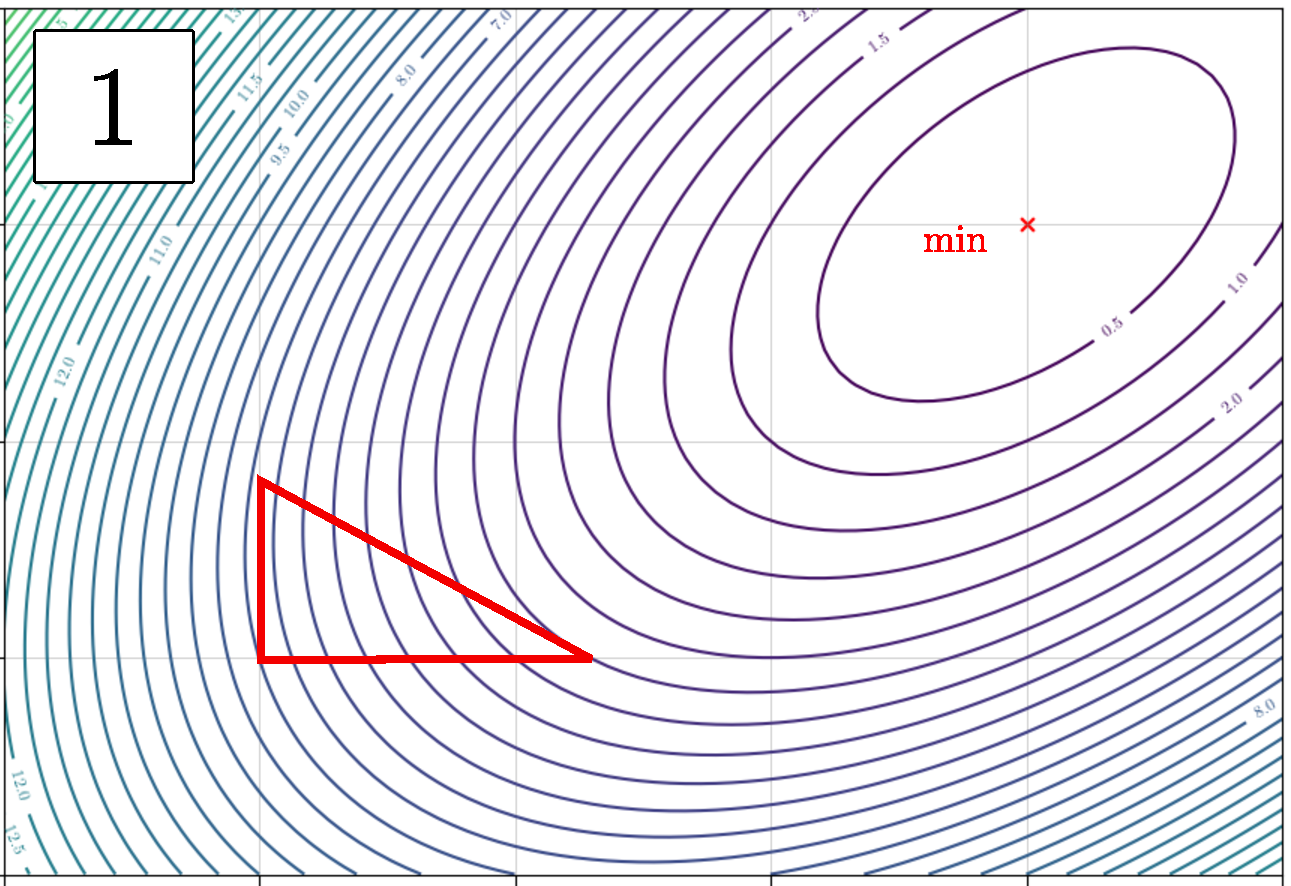
\includegraphics[width=0.96\textwidth, trim={0 0 0 0}, clip]{figures/nelder1.pdf}
	\end{subfigure}
	\begin{subfigure}[b]{0.325\textwidth}
		\centering
		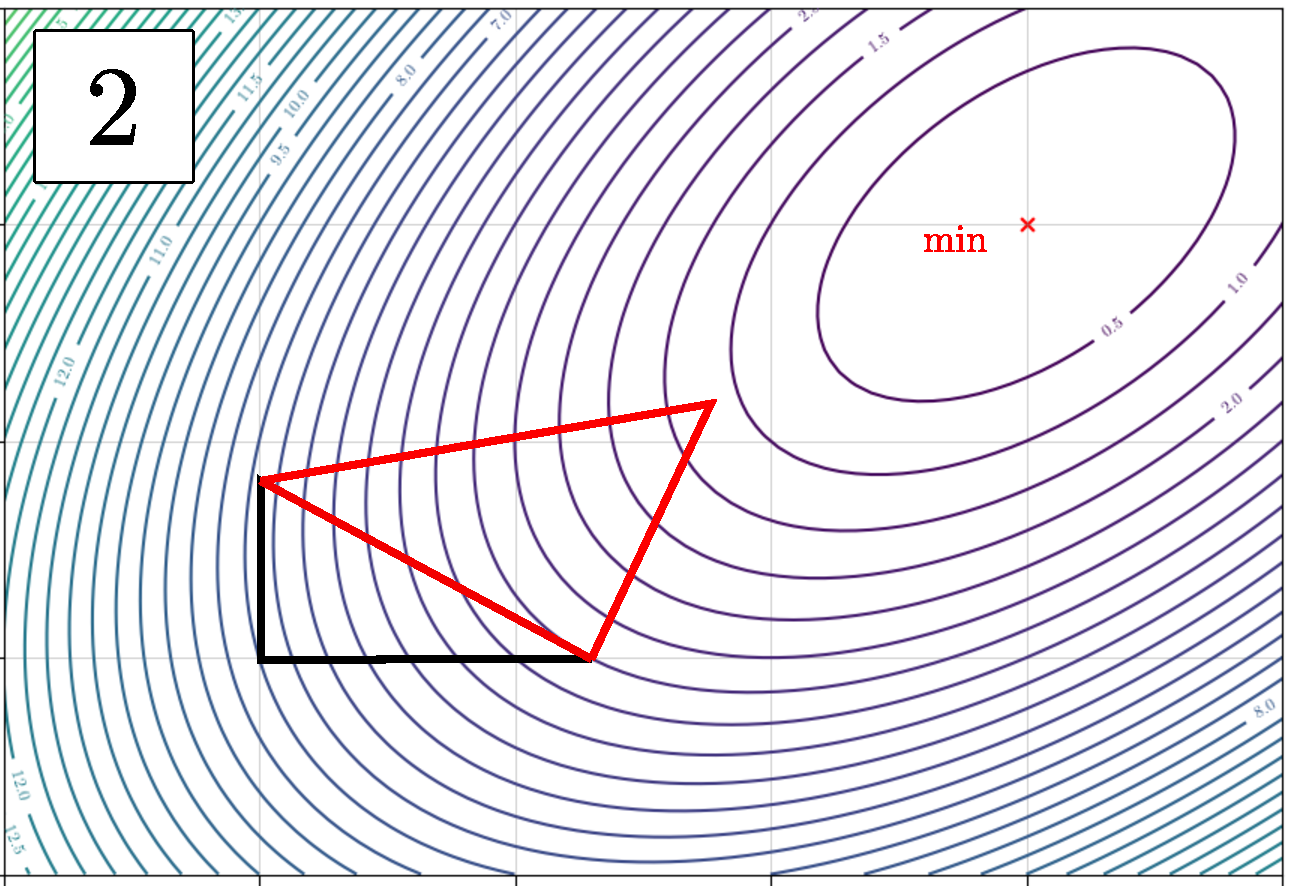
\includegraphics[width=0.96\textwidth, trim={0 0 0 0}]{figures/nelder2.pdf}
	\end{subfigure}
	\vspace{1mm}
	\begin{subfigure}[b]{0.325\textwidth}
		\centering
		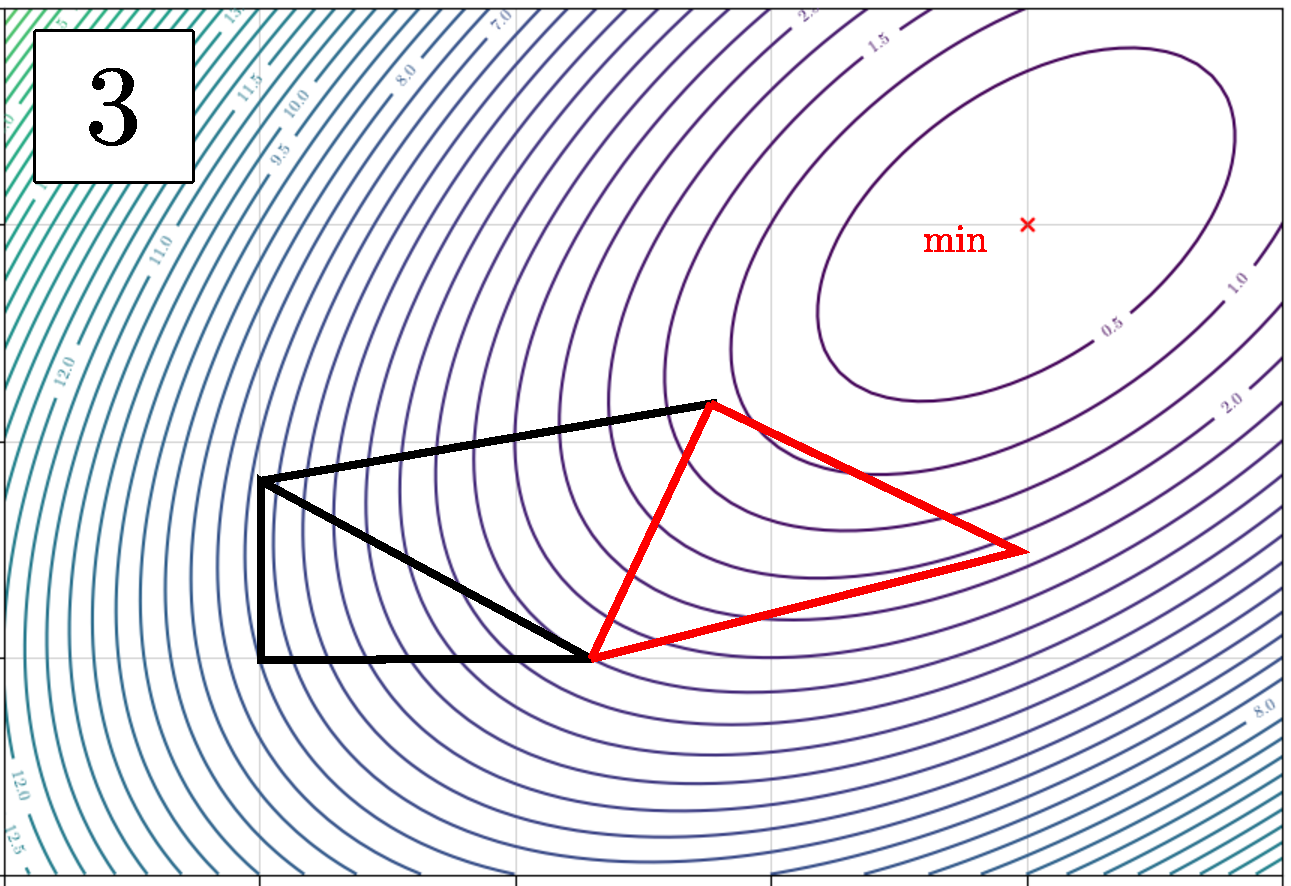
\includegraphics[width=0.96\textwidth, trim={0 0 0 0}]{figures/nelder3.pdf}
	\end{subfigure}
	\vspace{1mm}
	\begin{subfigure}[b]{0.325\textwidth}
		\centering
		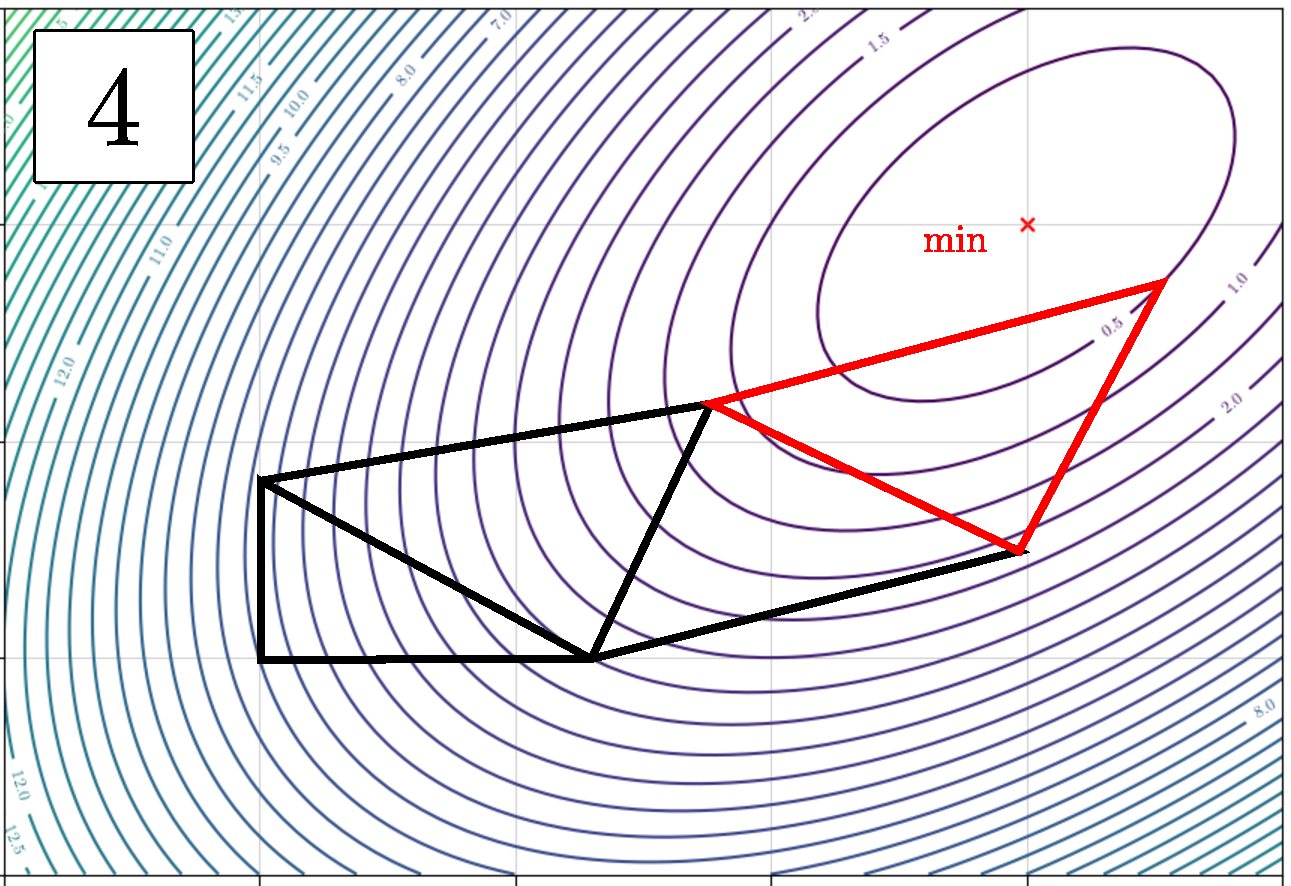
\includegraphics[width=0.96\textwidth, trim={0 0 0 0}]{figures/nelder4.pdf}
	\end{subfigure}
	\begin{subfigure}[b]{0.325\textwidth}
		\centering
		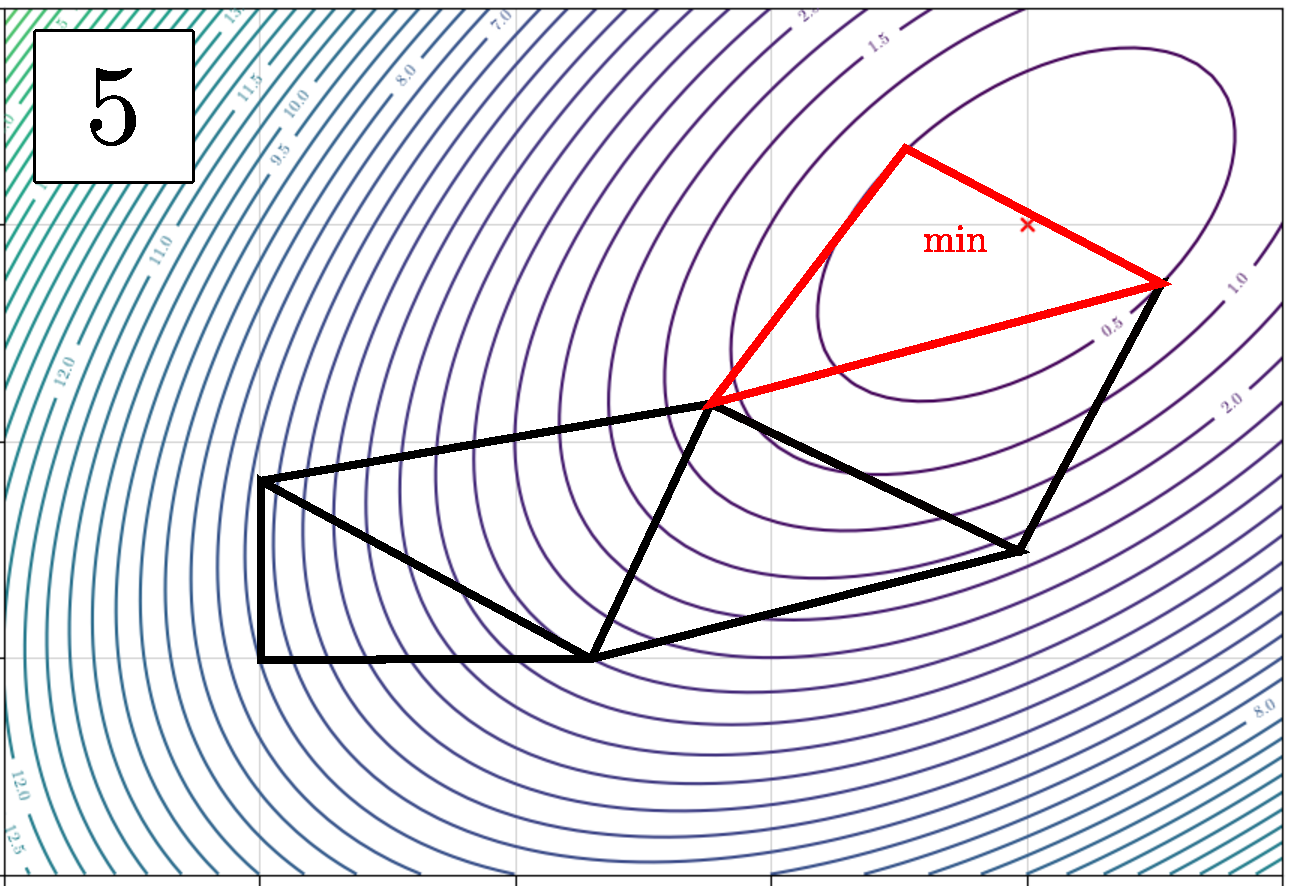
\includegraphics[width=0.96\textwidth, trim={0 0 0 0}]{figures/nelder5.pdf}
	\end{subfigure}
	\begin{subfigure}[b]{0.325\textwidth}
		\centering
		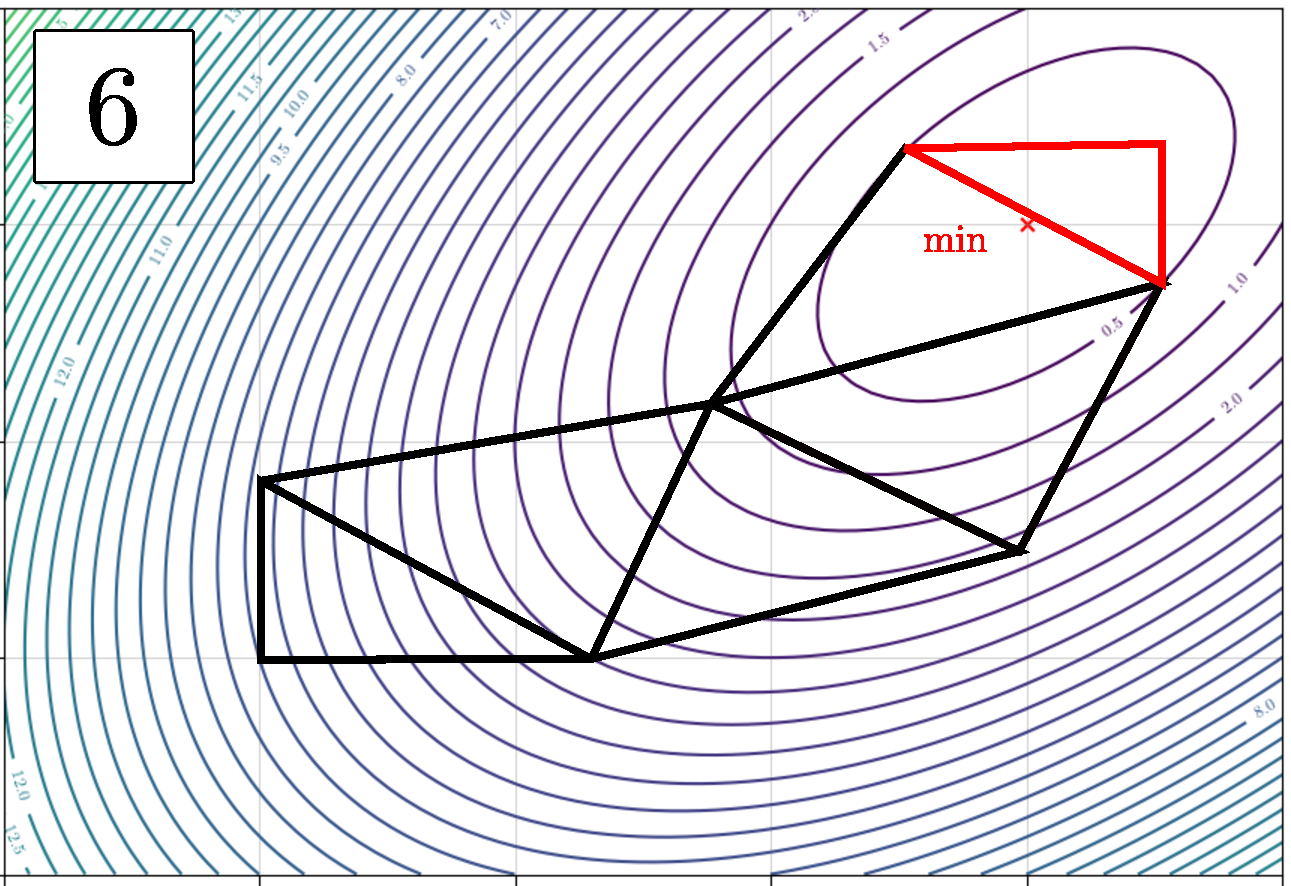
\includegraphics[width=0.96\textwidth, trim={0 0 0 0}]{figures/nelder6.pdf}
	\end{subfigure}
	\centering
	\begin{subfigure}[b]{0.325\textwidth}
		\centering
		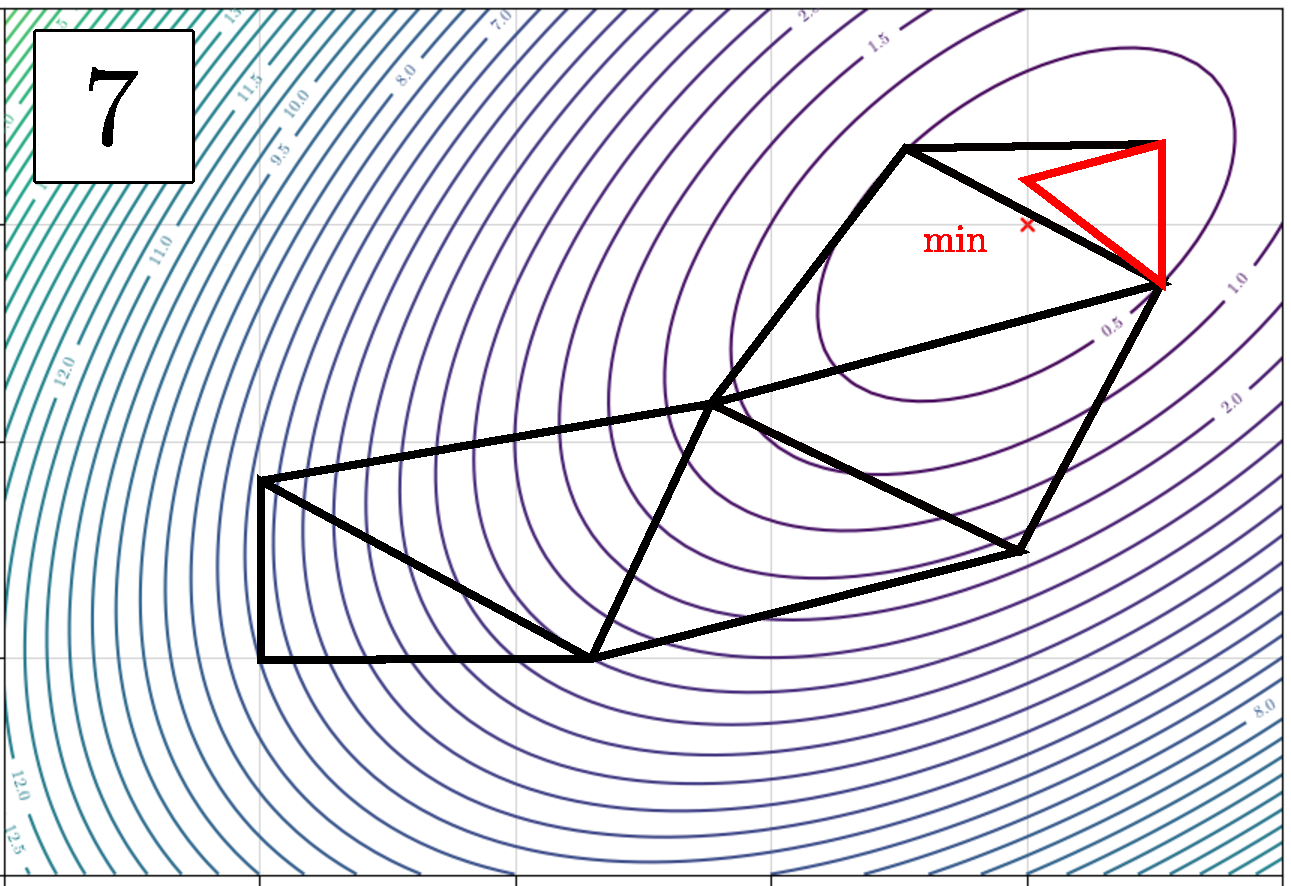
\includegraphics[width=0.96\textwidth, trim={0 0 0 0}]{figures/nelder7.pdf}
	\end{subfigure}
	\begin{subfigure}[b]{0.325\textwidth}
		\centering
		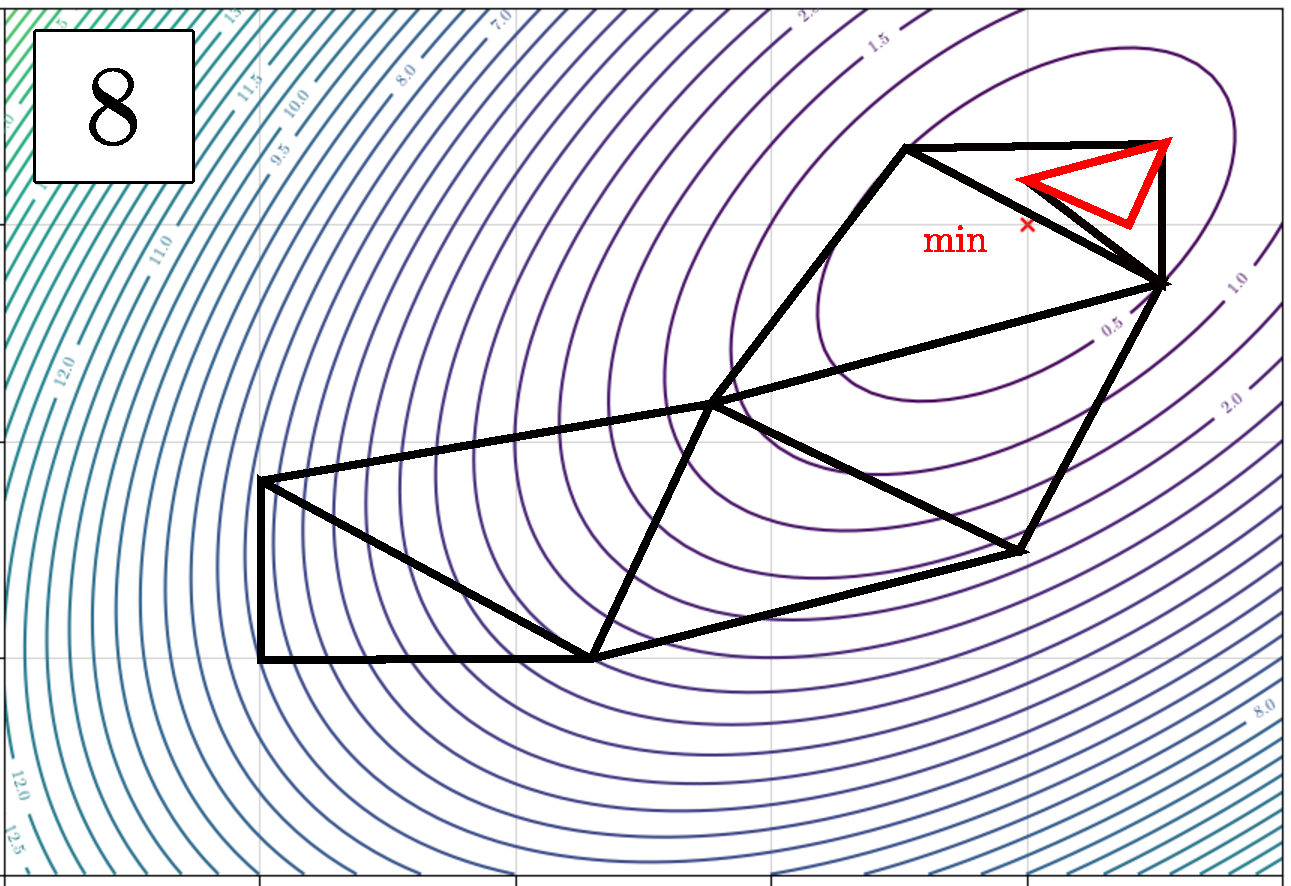
\includegraphics[width=0.96\textwidth, trim={0 0 0 0}]{figures/nelder8.pdf}
	\end{subfigure}
	\begin{subfigure}[b]{0.325\textwidth}
		\centering
		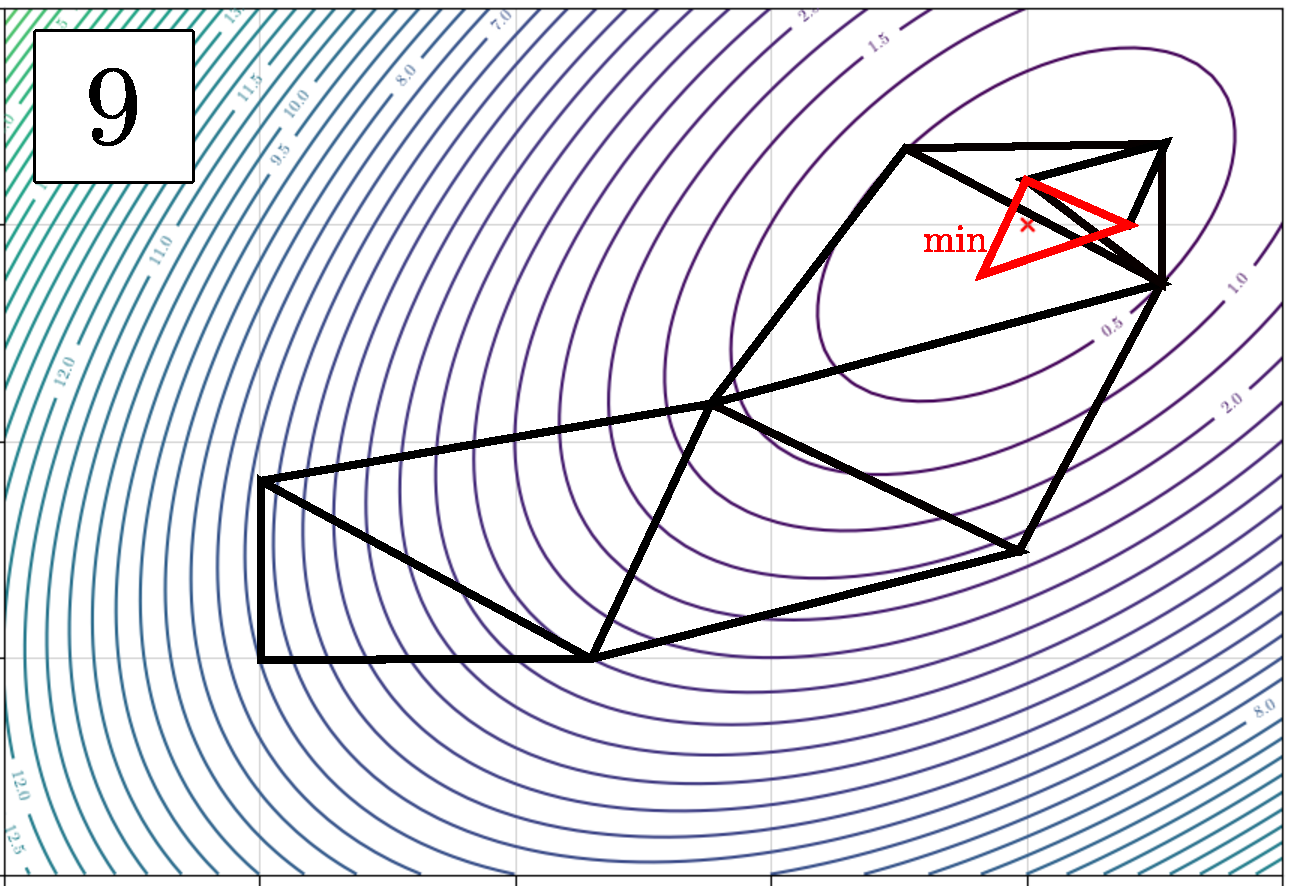
\includegraphics[width=0.96\textwidth, trim={0 0 0 0}]{figures/nelder9.pdf}
	\end{subfigure}
	\begin{center}
		\begin{subfigure}[b]{0.77\textwidth}
			\centering
			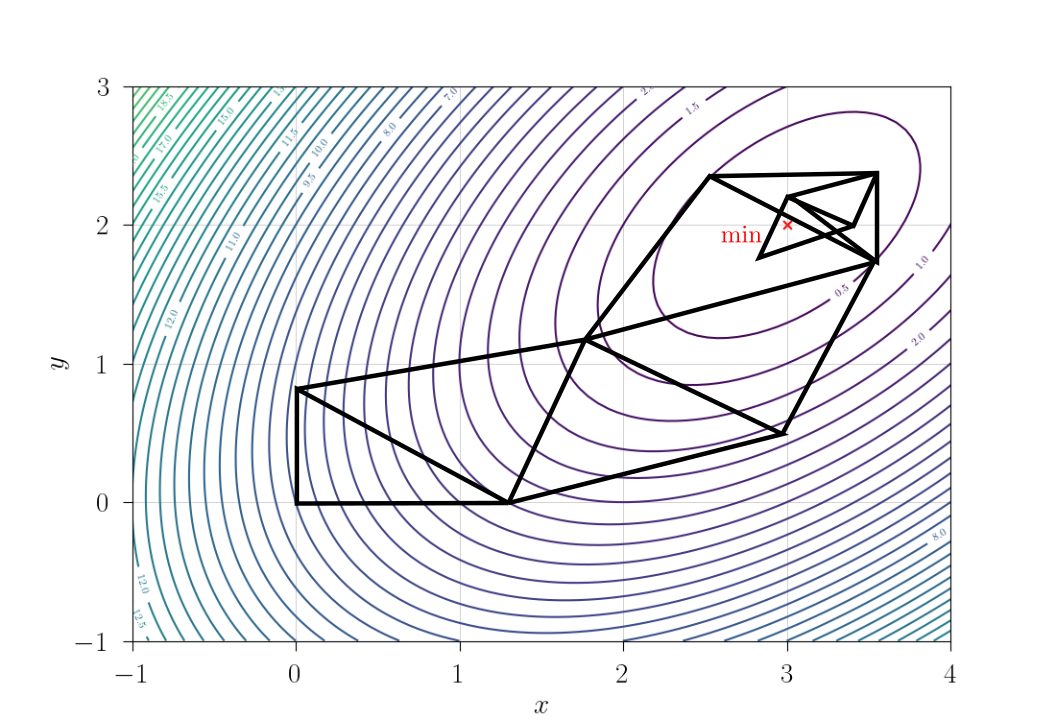
\includegraphics[width=0.985\textwidth, trim={0 6mm 0 7mm}]{figures/nelder.png}
		\end{subfigure}
	\end{center}
	
	\caption{Several iterations of the Nelder-Mead method for a specific choice of the initial simplex when minimizing the function $ x^2 - 4x + y^2 - y - xy + 7 $, with the minimum at the point (3,2) marked by a red cross.}
	\label{fig:NM}
\end{figure}


\subsection{Direct search methods}\label{direct-search}
In this part, we describe the \textit{generalized pattern search} (hereafter GPS) method \cite{Audet2002} and the \textit{mesh adaptive direct search} (hereafter MADS) method \cite{Audet2006}.

To describe the GPS algorithm, it is necessary to define a mesh, which is used to describe the search sets within the GPS algorithm. Let $ \mathbf{G} \in \mathbb{R}^{n \times n} $ be invertible and $ \mathbf{Z} \in \mathbb{Z}^{n \times p} $, $n, p \in \mathbb{N}$. Assume that every vector from $ \mathbb{R}^{n} $ can be expressed as a linear combination of the columns of matrix $ \mathbf{Z} $ (treated as vectors), such that all the coefficients in this linear combination are non-negative. Furthermore, let $ \mathbf{D} = \mathbf{G} \mathbf{Z} $. The mesh $ \mathbf{M} $ generated by $ \mathbf{D} $ centered at point $ \vec{x} $ is defined as
\begin{equation}
	\mathbf{M} = \left\{ \vec{x} + \delta \, \mathbf{D} y \, | \, y \in \mathbb{N}^p \right\},
\end{equation}
where $ \delta $ is called the mesh size parameter \cite{BBO-textbook, Audet2002}. In each iteration of the GPS algorithm, the shape of the mesh generally changes, as it is always centered at the point representing the best estimate in that iteration, and the size of the mesh step also changes. Let $ \vec{x}_k $ and $ \delta_k $ represent the estimate of the solution and the mesh size in the $ k $-th iteration, respectively. We 
then define the mesh in the $ k $-th iteration, denoted as $ \mathbf{M} _k $, as
\begin{equation}
	\mathbf{M} _k = \left\{ \vec{x}_k + \delta_k \, \mathbf{D} y \, | \, y \in \mathbb{N}^p \right\}.
\end{equation}
Note that the columns of matrix $ \mathbf{D} $, as defined above, can be interpreted as the possible directions in which the GPS algorithm searches the optimization space \cite{BBO-textbook, Audet2002}. Examples of search directions and meshes generated by different matrices $\mathbf{G}$ and $\mathbf{Z}$ are presented in Figure~\ref{fig:gps}.


\begin{figure}[H]
	\centering
	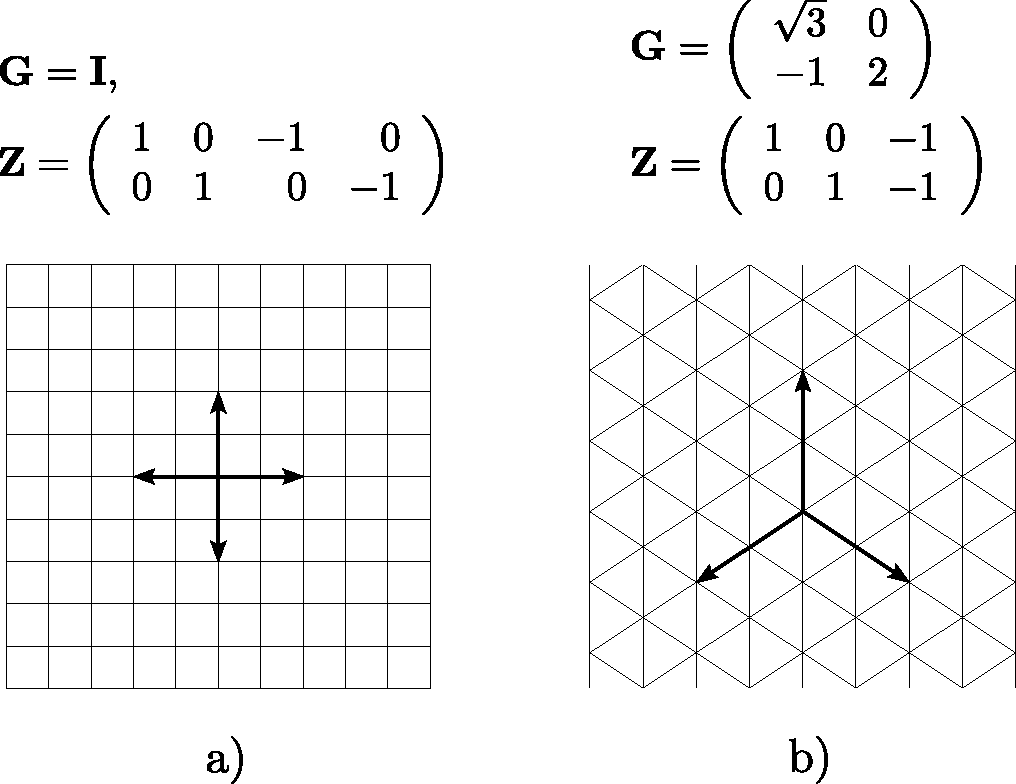
\includegraphics[width=0.70\textwidth]{figures/gps.pdf}
	\caption{Examples of search directions and meshes in $\mathbb{R}^2$ with
		obtained by different choices of $\mathbf{G}$ and~$\mathbf{Z}$. The mesh points
		are at the intersections of the lines, the arrows represent possible search directions.}
	\label{fig:gps}
\end{figure}


After initializing the necessary starting parameters, each iteration of the GPS algorithm is divided into two main steps. The first step is called the search step. During the search step, a finite set $S_k$ of candidate mesh points, selected according to a strategy specified by the user, is evaluated by computing the objective function at each one of the points. If none of the evaluated points represents an improvement over the value $ f(\vec{x}_k) $, the poll step follows. In the poll step, the objective function is evaluated at all neighboring mesh points of $ \vec{x}_k $. The poll set in $k$-th iteration is defined as $P_k = \{x_k + \delta_k d \, | \, d \in \mathbf{D}\}$. If none of the evaluated points represents an improvement over the value $ f(\vec{x}_k) $, we set $ \vec{x}_{k+1} = \vec{x}_k $ and decrease the mesh size, i.e., $ \delta_{k+1} < \delta_k $. However, if a point that improves the estimate of the solution is found in either the search or the poll step, this point is set as $ \vec{x}_{k+1} $, and the mesh size is increased, i.e., $ \delta_{k+1} > \delta_k $~\cite{BBO-textbook, Audet2002}.

The changes described above define a new mesh $ \mathbf{M} _k $ in each iteration. The mesh changes throughout the GPS algorithm. The algorithm terminates when $ \delta_{k+1} < \varepsilon $ for some user-specified $ \varepsilon > 0 $. It can be shown that the mesh step converges to zero, and under appropriate assumptions, the solution estimates converge to a stationary point of the objective function. Details can be found in \cite{BBO-textbook}. It should be noted that the convergence of GPS has been proven for unconstrained problems \cite{BBO-textbook}. The full GPS algorithm is presented in Algorithm~\ref{GPS-algo}.
\\[4pt]
\todo[inline]{Explain what is $t$ and $\tau$ in the algorithm, add typical ranges for $\tau$ maybe.}
\begin{algorithm}[H]
	\caption{Generalized Pattern Search (GPS) for unconstrained optimization}\label{GPS-algo}
	\begin{algorithmic}[1]
		\Require Function $f: \mathbb{R}^n \to \mathbb{R}$, initial point $x_0$, initial mesh size parameter $\delta_0$, positive spanning matrix $\mathbf{D}$, mesh size adjustment parameter $\tau \in (0, 1)$, stopping tolerance $\epsilon_{\text{stop}}$, iteration counter $k \gets 0$
		\Ensure Approximate optimal solution $\vec{x^{\star}}$ for function $f$
		
		\Procedure{GPS}{$x_0$}
		
		\While{$\delta_k > \epsilon_{\text{stop}}$}
		
		\Algphase{1. Search}
		\State Define a finite subset $S_k$ of the mesh $\mathbf{M}_k$
		\If{$f(t) < f(x_k)$ for some $t \in S_k$}
		\State Set $x_{k+1} \gets t$ and $\delta_{k+1} \gets \tau^{-1} \delta_k$
		\State \textbf{continue}
		\Else
		\State Go to Poll step
		\EndIf
		
		\Algphase{2. Poll}
		\State Select a positive spanning set $\mathbf{D}_k \subseteq \mathbf{D}$
		\State Define $P_k = \{x_k + \delta_k d : d \in \mathbf{D}_k\}$
		\If{$f(t) < f(x_k)$ for some $t \in P_k$}
		\State Set $x_{k+1} \gets t$ and $\delta_{k+1} \gets \tau^{-1} \delta_k$
		\Else
		\State $x_k$ is a mesh local optimizer
		\State Set $x_{k+1} \gets x_k$ and $\delta_{k+1} \gets \tau \delta_k$
		\EndIf
		
		\Algphase{3. Termination}
		\If{$\delta_{k+1} \leq \epsilon_{\text{stop}}$}
		\State \textbf{terminate}
		\Else
		\State Increment $k \gets k+1$ and continue
		\EndIf
		
		\EndWhile
		\EndProcedure
	\end{algorithmic}
\end{algorithm}

We turn our attention to the MADS algorithm, which generalizes the GPS algorithm by allowing for a different set of polling directions. The key difference is that MADS introduces the concept of a frame, which allows the poll directions to form a dense subset in $ \mathbb{R}^{n} $ as the algorithm progresses~\cite{BBO-textbook, derivative-free-review}. The frame $\mathbf{F}_k$ at iteration $k$ is defined as
\begin{equation}
	\mathbf{F}_k = \{ \vec{x} \in \mathbf{M}_k \ \big| \ \| \vec{x} - \vec{x}_k \|_\infty \leq \Delta_k b \},
\end{equation}
where $M_k$ represents the current mesh, $ \Delta_k $ is the frame size parameter, satisfying $ \delta_k \leq \Delta_k $, and $b = \max \ \{ \| d \| _\infty \ \big| \ d \in \mathbf{D} \}$. The extent of the frame is determined by the parameter $ \Delta_k $, and the polling directions are taken from this frame.

Each iteration of the MADS algorithm begins similarly to GPS, with a search step where a finite set $S_k$ of candidate points, selected based on the current mesh, is evaluated by computing the objective function at each of the points. If none of these points improves upon the current best solution, the algorithm proceeds to the poll step. 
 
The poll set $P_k$ is a subset of points selected from $\mathbf{F}_k$ and $\mathbf{M}_k$. Trivially, $P_k \subseteq \mathbf{F}_k \subseteq \mathbf{M}_k$. Importantly, the mesh size parameter $ \delta_k $ is allowed to decrease more rapidly than the  enabling the poll directions to asymptotically become arbitrarily dense~\cite{Audet2006}. This aspect is crucial, as it ensures that MADS can explore directions in a finer and more systematic manner than GPS, leading to better convergence properties.


\begin{figure}[H]
	\centering
	\vspace{0.5cm}
	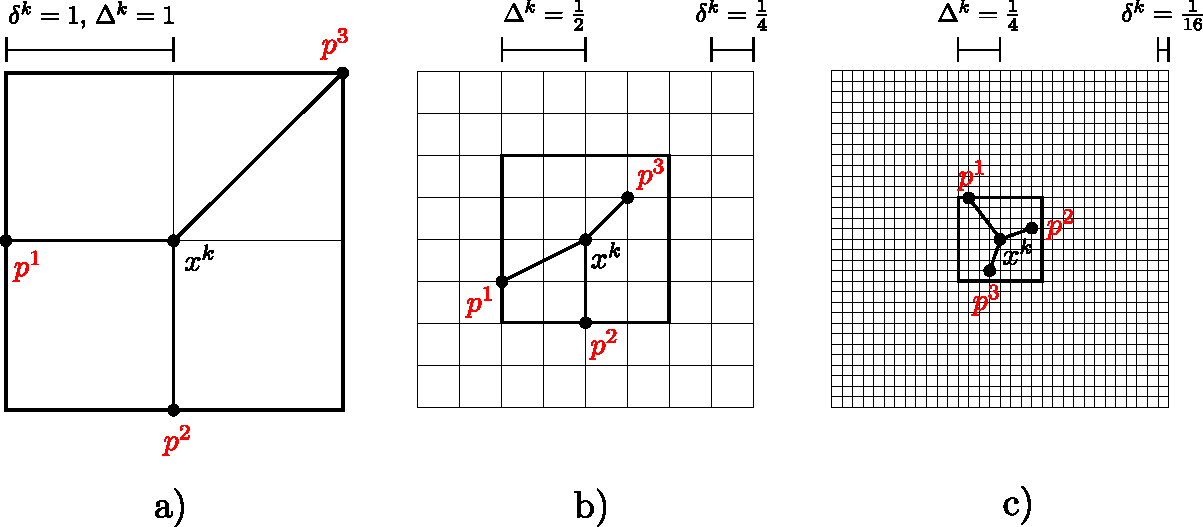
\includegraphics[width=1.01\textwidth]{figures/mads.pdf}
	\caption{Examples of meshes and frames $\mathbb{R}^2$ for different
		values of $\delta_k$ and $\Delta_k$}
	\label{fig:mads}
\end{figure}

If an improvement is found in the poll step, the new point is set as $ \vec{x}_{k+1} $, and the frame size $ \Delta_k $ and mesh size $ \delta_k $ may be increased to encourage further exploration. Conversely, if no improvement is found, $ \vec{x}_{k+1} = \vec{x}_k $, and the mesh size is reduced, i.e., $ \delta_{k+1} < \delta_k $, to allow for a more local search. The process of shrinking and refining the frame and mesh sizes continues until $ \delta_k $ falls below a user-specified threshold, at which point the algorithm terminates.

MADS also incorporates the \textit{extreme barrier function} to handle constraints, similarly to GPS. For constrained optimization problems, the objective function is modified into an extreme barrier function~\cite{BBO-textbook}, which penalizes any infeasible points by assigning them an infinite objective value. This simple yet effective strategy ensures that the optimization remains focused on feasible regions of the search space, and the algorithm converges to a stationary point even for constrained problems. A full description of the MADS algorithm and its implementation details can be found in~\cite{BBO-textbook}.



\begin{algorithm}[H]
	\caption{Mesh Adaptive Direct Search (MADS) for constrained optimization}\label{MADS}
	\begin{algorithmic}[1]
		\Require Function $f_{\infty}: \mathbb{R}^n \to \mathbb{R} \cup \{\infty\}$, initial point, initial frame size parameter $\Delta_0$, positive spanning matrix $\mathbf{D}$, mesh size adjustment parameter $\tau \in (0,1)$, stopping tolerance $\epsilon_{\text{stop}}$, iteration counter $k \gets 0$
		\Ensure Approximate optimal solution $\vec{x^{\star}}$ for function $f$
		
		\Procedure{MADS}{$x_0$}
		
		\While{$\Delta_k > \epsilon_{\text{stop}}$}
		
		\Algphase{1. Parameter Update}
		\State Set the mesh size parameter $\delta_k = \min \{\Delta_k, (\Delta_k)^2\}$
		
		\Algphase{2. Search}
		\State Define a finite set $S_k \subset \mathbf{M}_k$ such that:
		\If{$f_{\infty}(t) < f_{\infty}(x_k)$ for some $t \in S_k$}
		\State Set $x_{k+1} \gets t$ and $\Delta_{k+1} \gets \tau^{-1}\Delta_k$
		\State \textbf{continue}
		\Else
		\State Go to Poll step
		\EndIf
		
		\Algphase{3. Poll}
		\State Select a positive spanning set $\mathbf{D}_{k}$ and define:
		\State $P_k = \{x_k + \delta_k d : d \in \mathbf{D}_{k}\}$, a subset of the frame $\mathbf{F}_k$ with extent $\Delta_k$
		\If{$f_{\infty}(t) < f_{\infty}(x_k)$ for some $t \in P_k$}
		\State Set $x_{k+1} \gets t$ and $\Delta_{k+1} \gets \tau^{-1}\Delta_k$
		\Else
		\State Set $x_{k+1} \gets x_k$ and $\Delta_{k+1} \gets \tau\Delta_k$
		\EndIf
		
		\Algphase{4. Termination}
		\If{$\Delta_{k+1} \leq \epsilon_{\text{stop}}$}
		\State \textbf{terminate}
		\Else
		\State Increment $k \gets k+1$ and continue
		\EndIf
		
		\EndWhile
		\EndProcedure
	\end{algorithmic}
\end{algorithm}
\subsection{Optimization Using a Surrogate Model}\label{model-based}
In cases where evaluating the objective function at a specific point is time-consuming or computationally expensive, it can be useful to employ a surrogate model for the objective function during optimization. We define a surrogate model of the given problem as the problem

\begin{equation}
	\min_{\vec{x} \in \mathbf{\tilde{X}}} \tilde{f}(\vec{x}),
\end{equation}
where
\begin{equation}
	\mathbf{\tilde{X}} = \left\{ \vec{x} \in \mathbf{D} \subseteq \mathbb{R}^n \ \middle| \ \vec{\tilde{g}} (\vec{x}) \leq \vec{0} \wedge \vec{\tilde{h}} (\vec{x}) = \vec{0} \right\},
\end{equation}
and the functions \( \tilde{f}, \vec{\tilde{g}} \), and \( \vec{\tilde{h}} \) have characteristics similar to those of the functions \( f, \vec{g} \), and \( \vec{h} \) in the original problem. The characteristics of \( \tilde{f}, \vec{\tilde{g}} \), and \( \vec{\tilde{h}} \) are intentionally left undefined, reflecting the fact that the surrogate model does not necessarily need to be an accurate approximation of the original problem \cite{BBO-textbook, two-decades, Kramer2011}. A good approximative model may not always be a suitable surrogate for optimization purposes, a situation illustrated in Figure \ref{fig:surrogate}.

\begin{figure}[H]
	\centering
	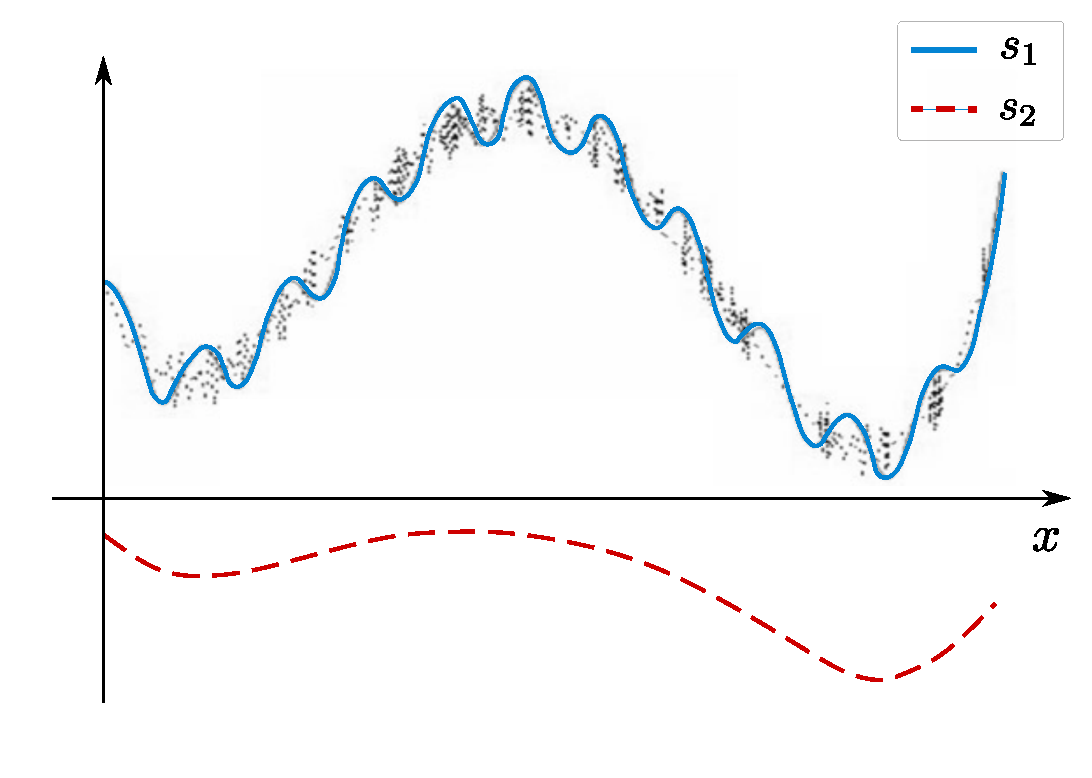
\includegraphics[width=0.6\textwidth]{figures/surrogate.pdf}
	\caption{An illustration of two surrogate models, $ s_1 $ and $ s_2 $. The black points represent noisy values of the objective function. While using surrogate model $ s_1 $ represents a better choice for approximating the function, it is not suitable for optimization since $ s_1 $ contains many undesirable stationary points that the original objective function does not have. On the other hand, while surrogate model $ s_2 $ is not as accurate in approximating the function's values, it is a better choice for optimization because the stationary points of $ s_2 $ are almost identical to those of the optimized objective function.}
	\label{fig:surrogate}
\end{figure}

Using a surrogate model in optimization is often just a part of a more complex optimization method. Surrogate models can, for example, be used within GPS and MADS methods described in section \ref{direct-search}, where, during the poll step, we first evaluate the surrogate function \( \tilde{f} \) at the points from the poll set, sort these values, and use them to sort the poll set used to evaluate the original function \( f \). This potentially allows us to significantly reduce the time required to complete the poll step, as sorting the points increases the probability of finding a better estimate of the solution at one of the first examined points \cite{BBO-textbook}. Surrogate models can also be used within other methods to accelerate the optimization process, and their application is discussed in detail in \cite{BBO-textbook, two-decades}.

\section{Description of the optimization framework}\label{framework}
A fully automated and modular optimization framework was developed to solve the optimization problems in this work. The proposed framework is composed of several components, which are described in detail below:

\begin{enumerate}
	\item \textbf{Optimization}:  
	The first component encompasses the optimization method, which governs the entire process. In this part, the optimization problem is defined along with any required constraints.
	
	In this study, we use the Nelder-Mead method, implemented in Python specifically for this work and detailed in Appendix~\ref{appendix B}. Additionally, the framework includes the MADS method (see Section~\ref{direct-search}), implemented in the open-source \texttt{NOMAD} library \cite{nomad} in C++. For handling constraints in both the Nelder-Mead and MADS methods, we use the extreme barrier function.
	
	\item \textbf{Geometry Generation}:  
	The optimization parameters, updated at each iteration, are passed to the geometry generator. For generating the geometries used in numerical simulations, we use the \texttt{meshgen} package detailed in Chapter~\ref{geometry}.
	
	\item \textbf{Numerical Simulation}:  
	The final component of the optimization framework is the numerical solver, which evaluates the objective function based on the generated geometry. Numerical simulations are performed using the LBM, which is described alongside additional implementation details in Chapter~\ref{lbm}.
\end{enumerate}

The interconnection of these components within the optimization framework is schematically illustrated in Figure~\ref{fig:framework}.


\begin{figure}[H]
	\vspace{5mm}
	\centering
	\includegraphics[width=0.95\textwidth]{figures/framework-en.pdf}
	\vspace{5mm}
	\caption{Schematic representation of the modular optimization framework. It consists of three main components: (1) Optimization, which defines the problem and governs the iterative process, (2) Geometry generation, where optimization parameters are translated into geometric models using \texttt{meshgen}, and (3) Numerical simulation, where the objective function is evaluated using the LBM.}
	\label{fig:framework}
	
\end{figure}
\chapter{Results}\label{results}

In this chapter, we analyze two proposed idealized models of the TCPC. These models are designed to incorporate key geometric modifications identified as beneficial in reducing energy dissipation, as described in \cite{Rijnberg2018}. These modifications, summarized in Figure~\ref{fig:positive_modifications}, serve as a foundation for investigating the effects of caval offsetting, curving, flaring, and other geometric factors on flow dynamics.

\begin{figure}[H]
	\centering
	\includegraphics[width=0.65\textwidth]{figures/energyloss-en.pdf}
	\caption[Positive Modifications for TCPC]{Key modifications to improve TCPC geometry and reduce energy dissipation: (a) caval offsetting, where the inferior and superior vena cava are misaligned to minimize flow collision; (b) curving, where the conduits are curved to enhance flow alignment; (c) the Y-graft configuration, which splits the flow evenly between outlets; and (d) flaring, where the connections are widened to reduce sharp corners and flow resistance. Adapted from \cite{Rijnberg2018}.}
	\label{fig:positive_modifications}
\end{figure}

\section{The Models}

To systematically evaluate the effects of geometric changes, the models were developed with varying levels of complexity, incorporating different numbers of degrees of freedom. Both models represent idealized TCPC geometries and share the same labeling convention for inlets and outlets. Specifically, the inlets are denoted as $\Gamma^{N}_{\text{in}}$ (top inlet representing the superior vena cava) and $\Gamma^{S}_{\text{in}}$ (bottom inlet representing the inferior vena cava with the conduit). The outlets are labeled as $\Gamma^{W}_{\text{out}}$ (left outlet representing the left pulmonary artery) and $\Gamma^{E}_{\text{out}}$ (right outlet representing the right pulmonary artery). The shared geometric framework, along with labeled boundaries, is illustrated in Figure~\ref{fig:junction schema}.

\begin{figure}[H]
	\centering
	\begin{subfigure}{0.45\textwidth}
		\centering
		\includegraphics[width=0.75\textwidth, trim={0mm -13mm 0mm 0mm}]{figures/3dschema.pdf}
		\caption{3D schematic of the idealized TCPC junction.}
		\label{fig:schema 3d}
	\end{subfigure}\hspace{2mm}
	\begin{subfigure}{0.53\textwidth}
		\centering
		\includegraphics[width=0.99\textwidth, trim={0mm -5mm 0mm 0mm}]{figures/2dschema.pdf}
		\caption{2D schematic of the idealized TCPC junction, highlighting labeled boundaries.}
		\label{fig:schema 2d}
	\end{subfigure}
	\vspace{2mm}
	\caption[Schematic of Idealized TCPC Geometry]{2D and 3D schematic illustrations of the idealized TCPC geometry, showing labeled inlets ($\Gamma^{N}_{\text{in}}$, $\Gamma^{S}_{\text{in}}$) and outlets ($\Gamma^{W}_{\text{out}}$, $\Gamma^{E}_{\text{out}}$).}
	\label{fig:junction schema}
\end{figure}


\subsection{Model 1: Simplified Cylindrical Junction}

The first model represents a basic cylindrical junction, where the bottom vertical cylinder corresponds to the inferior vena cava (IVC), the horizontal cylinder corresponds to the pulmonary artery, and the top vertical cylinder represents the superior vena cava (SVC). The IVC and SVC are connected perpendicularly to the pulmonary artery, creating a cross-like structure. 

Model 1 was chosen because it introduces only one degree of freedom: the vertical offset of the IVC relative to the SVC. This simplicity makes it feasible to sample and evaluate the optimization space exhaustively, providing an opportunity to study the behavior of the objective functions, namely wall shear stress (WSS) and turbulence kinetic energy (TKE), in detail.

\begin{figure}[H]
	\centering
	\includegraphics[width=0.8\textwidth]{figures/krizovatka-obecna.pdf} % Replace with your figure for Model 1
	\caption[Simplified Cylindrical Junction]{Schematic of Model 1: A simplified cylindrical junction with one degree of freedom, the vertical offset of the IVC relative to the SVC.}
	\label{fig:model1_schematic}
\end{figure}

\subsection{Model 2: Complex Geometric Model}

The second model introduces additional complexity by incorporating five degrees of freedom: the vertical offset of the IVC, the angles of connection for both the IVC and SVC to the pulmonary artery, the flaring of the IVC, and the width of the IVC. This model enables a more detailed investigation of the interaction between geometric parameters and hemodynamic efficiency.

Model 2 was selected because its higher complexity allows for greater variations in geometry and, consequently, a potentially larger impact on flow dynamics. However, the increased number of degrees of freedom makes it infeasible to sample the optimization space comprehensively, rendering the model more akin to a "black box" during optimization.

\begin{figure}[H]
	\centering
	\includegraphics[width=0.8\textwidth]{figures/krizovatka-obecna.pdf} % Replace with your figure for Model 2
	\caption[Complex Geometric Model]{Schematic of Model 2: A more complex model with five degrees of freedom—IVC offset, connection angles, flaring, and width of the IVC.}
	\label{fig:model2_schematic}
\end{figure}

\section{Objective functions and other monitored quantities}
Selecting appropriate objective functions is essential for guiding geometric optimization. In this work, we focus primarily on two such functions: the turbulence kinetic energy (TKE) and the shear rate near the walls. In addition, we also present other relevant metrics that are monitored during the computations.

\subsubsection*{Turbulence kinetic energy}
TKE, defined by~\eqref{eq:turb kin energy}, measures the intensity of velocity fluctuations within the flow. In the context of the TCPC, higher TKE generally corresponds to increased energy losses. Thus, reducing TKE in the TCPC region is desirable in order to improve hemodynamic efficiency. We sum TKE over a defined control volume within the computational domain, obtaining a global level of turbulent activity in the region. In the case of TCPC, TKE can serve as surrogate measure of how smoothly and efficiently blood flows through the connection.

\subsubsection*{Shear rate}
Shear rate, defined in \eqref{eq:dot gamma}, provides insight into the mechanical forces acting on the vessel walls. Excessive shear rate can negatively affect the vascular health, making controlling near-wall shear rates crucial for ensuring the long-term patency and physiological compatibility of the TCPC.

However, measuring shear rate directly at the wall in a computational framework -- especially using LBM -- poses a challenge. The discrete nature of the grid and the no-slip boundary condition mean that the resolution near the wall can affect the computed shear rate and make it sensitive to discretization details. To address this, we introduce a thin layer of thickness 1 mm adjacent to the vessel walls. Within this layer, we sum the shear rate values rather than relying solely on the cells immediately neighboring the walls. This approach was chosen to reduce the sensitivity on grid characteristics while maintaining the physiological relevance of the quantity, ensuring it provides representative measure of local flow behavior.

\subsubsection*{IVC flow split}
In addition to the main objective functions, we monitor how fluid from the inferior vena cava divides between the left and right pulmonary arteries. A balanced or at least minimally maintained split of inferior vena cava flow into both pulmonary artery branches is desirable. This metric is evaluated in post-processing using the computed mean velocity field.

\subsubsection*{Mean velocity vector angle at the pulmonary artery outlets}
It is beneficial for blood in the pulmonary arteries to flow downstream in a laminar manner. Thus, we examine the angle between the mean velocity vector and the outlet normal vector. This angle provides the information  for studying the laminarity of the flow.

\section{The models}

To systematically evaluate the effects of geometric changes, the models were developed with varying levels of complexity, incorporating different numbers of degrees of freedom. Both models represent idealized TCPC geometries and share the same labeling convention for inlets and outlets. 

The inlets are denoted as $\Gamma^{\text{N}}_{\text{in}}$ (representing the superior vena cava at the top) and $\Gamma^{\text{S}}_{\text{in}}$ (representing the inferior vena cava with the conduit at the bottom). Similarly, the outlets are labeled as $\Gamma^{\text{W}}_{\text{out}}$ (representing the left part of the pulmonary artery) and $\Gamma^{\text{E}}_{\text{out}}$ (representing the right part of the pulmonary artery).
The shared geometric framework and boundary labels, is illustrated in Figure~\ref{fig:junction schema}. The dimensions of cylindrical segments forming the simplified junction are presented in Table~\ref{tab:tcpc dims}.


\begin{figure}[H]
	\centering
	\vspace{2mm}
	\includegraphics[width=0.99\textwidth]{figures/3d-tcpc-schema-combined.pdf}
	\vspace{7mm}
	\caption{Schematic representation of the idealized TCPC geometry. The labeled inlets ($\Gamma^{\text{N}}_{\text{in}}$, $\Gamma^{\text{S}}_{\text{in}}$) and outlets ($\Gamma^{\text{W}}_{\text{out}}$, $\Gamma^{\text{E}}_{\text{out}}$), directions of inflows and outflows, and the dimensions of the cylindrical segments forming the junction are illustrated.}
	\label{fig:junction schema}
\end{figure}

\bgroup
\centering
\vspace{4mm}
\setlength\tabcolsep{3mm}
\def\arraystretch{1.7}%
\begin{tabular}{|l|l|c|c|}
	\hline
	Segment & Abbreviation & Length & Diameter \\ \hline
	Inferior vena cava 	& IVC 	&      39 mm        &     14 mm    \\ 
	Superior vena cava  & SVC 	&      39 mm     	&     14 mm     \\ 
	Pulmonary artery 	& PA 	&      170 mm     	&     22 mm     \\  \hline
\end{tabular}
\vspace{2mm}
\captionof{table}{Dimensions of the cylindrical segments forming the idealized TCPC junction.}
\vspace{4mm}
\label{tab:tcpc dims}
\egroup

In both models, the objective functions are studied within a defined control volume, denoted as A, which is a subset of the entire computational domain. By restricting the analysis to this region, we aim reduce potential errors introduced by the numerical boundary conditions. The control volume involves inlet and outlet boundaries named according to their respective vessel segments: \(\Gamma^{\text{SVC}}_{\text{in}}\) for the superior vena cava inlet, \(\Gamma^{\text{IVC}}_{\text{in}}\) for the inferior vena cava inlet, \(\Gamma^{\text{LPA}}_{\text{out}}\) for the left pulmonary artery outlet, and \(\Gamma^{\text{RPA}}_{\text{out}}\) for the right pulmonary artery outlet. The turbulence kinetic energy is evaluated in the entire control volume. The near-wall shear rate is examined along the boundaries of the control volume that are shared with the vessel walls.

\subsection*{Model 1: Simplified cylindrical junction}\label{mod:model1}
The first model represents a basic cylindrical junction where the IVC and SVC are connected perpendicularly to the PA, forming a cross-like structure, as illustrated in Figure~\ref{fig:model1_schematic}. Model 1 was chosen because it introduces only one degree of freedom, the horizontal offset of the IVC axis relative to the SVC, denoted by $o_1$. This simplicity makes it possible to sample the optimization space and evaluate the objective functions at the points of the sampling. This provides an opportunity to examine the behavior of the objective functions and verify the result generated by the optimization framework.

\subsection*{Model 2: More complex geometric model}\label{mod:model2}
Illustration of Model 2 is presented in Figure~\ref{fig:model1_schematic}. The second model introduces additional complexity by incorporating six degrees of freedom:
\begin{itemize}
	\item horizontal offset of the IVC axis, denoted by $o_1$,
	\item angle of the IVC axis, denoted by $\alpha_1$,
	\item angle of the SVC axis, denoted by $\alpha_2$,
	\item width and curvature of the IVC-PA connection, denoted by $f_1$,
	\item width and curvature of the SVC-PA connection, denoted by $f_2$,
	\item width of the IVC, denoted by $l_1$.
\end{itemize}
Model 2 was selected because its higher complexity allows for more geometric variations.

\begin{figure}[H]
	\begin{subfigure}{0.48\textwidth}
		\centering
		\includegraphics[width=0.91\textwidth, trim={0 0 0 0}]{figures/model1.pdf}
		\caption[Simplified Cylindrical Junction]{Schematic of Model 1: A simplified cylindrical junction with one degree of freedom, the horizontal offset of the IVC.}
		\label{fig:model1_schematic}
	\end{subfigure}\hfill%
	\begin{subfigure}{0.48\textwidth}
		\centering
		\includegraphics[width=0.91\textwidth]{figures/model2.pdf}
		\caption[Complex Geometric Model]{Schematic of Model 2: A more complex model introducing six degrees of freedom: IVC offset and width, connection angles and flaring.}
		\label{fig:model2_schematic}
	\end{subfigure}
	\vspace{4mm}
	\caption{Schematic illustrations of Model 1 and Model 2.}
	\label{fig:model schemas}
\end{figure}
\section{Problem with one optimization parameter}\label{optim1}
In this section, we focus on a simplified model of the TCPC in a form of a basic cylindrical junction to investigate the behavior of key hemodynamic quantities under varying caval offset. The problem setup is defined in Problem Setup \hyperlink{page.48}{1}. The dimensions of the domain, the value of the kinematic viscosity, and the value of the inflows are chosen to mimic real values occurring in physiological conditions \cite{Rijnberg2018}.

\vspace{2mm}
\begin{problem}{Basic cylindrical junction}
	\vspace{2mm}
	Physical setup:
	\begin{itemize}
		\item Domain: $ \Omega=(0 ; 170 \mathrm{~mm}) \times(0 ; 22 \mathrm{~mm}) \times(0 ; 100 \mathrm{~mm})$.
		\item Kinematic viscosity: $ \nu=3 \cdot 10^{-6} \mathrm{~m}^{2} \mathrm{~s}^{-1}$.
		\item Inflow at $\Gamma^{\text{IVC}}_{\text{in}}$: a constant velocity of magnitude $0{,}45$ \si{m s^{-1}},  aligned with the IVC axis in the positive $x_3$-direction.
		\item Inflow at $\Gamma^{\text{SVC}}_{\text{in}}$: a constant velocity of magnitude $0{,}35$ \si{m s^{-1}}, aligned with the SVC axis in the negative $x_3$-direction.
	\end{itemize} 
	LBM setup:
	\begin{itemize}
		\item Initial condition on $ \overline{\hat{\Omega}} $ set as described in Section~\ref{pocatecni podminka}.
		\item Boundary conditions at $\Gamma^{\text{W}}_{\text{out}}$ and $\Gamma^{\text{E}}_{\text{out}}$ set according to Section~\ref{symmetric bc}.
		\item Discretization: $\overline{\hat{\Omega}} = N_{x} \times N_{y} \times N_{z}$, $N_{x} = 768, \, N_{y} = 105, N_{z} = 453$.
		\item Kinematic viscosity in lattice units: $\nu^{L} = 10^{-3} $.
	\end{itemize}
	
\end{problem}

\subsection{Analysis of the system}
The main objective of this study is to minimize two studied quantities, $\dot{\gamma}^{A}_{\mathrm{nw}}$ and $T^{A}_{\mathrm{turb}}$. To study the system's behavior and to validate the result generated by the optimization framework, we systematically sample the optimization space prior to running the optimization algorithm.

Specifically, we discretize the $o_1$-parameter space with regular intervals of $0{,}1$ cm over the range $[0{,}1 \, \mathrm{cm}; 2{,}4 \, \mathrm{cm}]$, creating a set of sampling points
\begin{equation}
	P = \Big\{ \, \text{P}_i \, \big| \, i=0,1,2, \dots, 24 \, \Big\} = \Big\{ \, 0{,}1 \cdot i \: \big| \, i=0,1,2, \dots, 24 \, \Big\} \, .
\end{equation}
At each point of $P$, the system's response is evaluated by computing different flow characteristics. This study serves two purposes:
\begin{itemize}
	\item It provides insight into the system's behavior. Studying different geometrical setups helps with understanding of how flow characteristics vary with the changing value of parameter~$o_1$.
	\item By analyzing the sampled data, we can validate the performance of the optimization framework.
\end{itemize}
The results of the functions evaluations in the points of sampling are presented in Figure~\ref{fig:summary_metrics}.


\newgeometry{top=4.0cm}
\begin{figure}[H]
	\centering
	\begin{subfigure}{0.49\textwidth}
		\centering
		\includegraphics[
		width=\textwidth,
		trim={0mm 0mm 0mm 0mm}
		]{figures/mean_stress_3_interpolated.pdf}
		\caption{Near-wall shear rate ($\dot{\gamma}^{A}_{\mathrm{nw}}$) in lattice units, with the green region indicating flow from the IVC exceeding~25\%.}
		\label{fig:shear_rate}
	\end{subfigure}\hfill%
	\begin{subfigure}{0.49\textwidth}
		\centering
		\includegraphics[
		width=\textwidth,
		trim={0mm 0mm 0mm 0mm}
		]{figures/mean_turbulence_kinetic_energy_interpolated.pdf}
		\caption{Turbulent kinetic energy ($T^{A}_{\mathrm{turb}}$) in lattice units, with the green region indicating flow from the IVC exceeding~25\%.}
		\label{fig:tke}
	\end{subfigure}
	\\[10pt]
	\begin{subfigure}{0.49\textwidth}
		\centering
		\includegraphics[
		width=\textwidth,
		trim={0mm 0mm 0mm 0mm}
		]{figures/svc_lpa.pdf}
		\vspace{4mm}
		\caption{Percentage of flow directed from the SVC to the LPA (green dashed line) and RPA (orange dashed line).}
		\label{fig:svc_flow_split}
	\end{subfigure}\hfill%
	\begin{subfigure}{0.49\textwidth}
		\centering
		\includegraphics[
		width=\textwidth,
		trim={0mm 0mm 0mm 2.0mm}
		]{figures/ivc_lpa.pdf}
		\vspace{5mm}
		\caption{Percentage of flow directed from the IVC to the LPA and RPA. The red region highlights offsets where the flow fraction to the LPA is below 25\%.}
		\label{fig:ivc_flow_split}
	\end{subfigure}
	\begin{center}
		\vspace{-30mm}
		\includegraphics[
		width=0.25\textwidth,
		trim={0mm 0mm 0mm 0mm}
		]{figures/ivc-svc-leg.png}
		\vspace{20mm}
	\end{center}
	\vspace{2mm}
	\caption{Summary of key analyzed metrics. (a) Near-wall shear rate ($\dot{\gamma}^{A}_{\mathrm{nw}}$) in lattice units, with green region indicating offsets for which IVC-LPA flow exceeds 25\%; (b) Turbulent kinetic energy ($T^{A}_{\mathrm{turb}}$) in lattice units, with similar IVC-LPA flow threshold; (c) Flow distribution from the SVC to the LPA and the RPA; (d) Flow distribution from the IVC to the LPA and RPA, with the red region indicating offsets where IVC-LPA flow is below 25\%.}

	\label{fig:summary_metrics}
\end{figure}
\restoregeometry
\newpage

Figure~\ref{fig:shear_rate} shows the near-wall shear rate $\dot{\gamma}^{A}_{\mathrm{nw}}$ as a function of $o_1$. At~$o_1 = 0{,}0 \, \mathrm{cm}$, where the geometry is perfectly symmetric, the shear rate is comparatively lower than it is for slightly larger offsets. Notably, we can observe sharp decrease to a local minimum at~$o_1 = 0{,}7 \, \mathrm{cm}$, i.e., an offset almost equal to 0{,}5-diameter of the IVC.  Subsequently, the shear rate exhibits a slight increase and then steadily declines to minimal values at higher offsets--around 1{,}5-diameter of the IVC.

The turbulent kinetic energy $T^{A}_{\mathrm{turb}}$ is shown in Figure~\ref{fig:tke}. At $o_1 = 0{,}0 \, \mathrm{cm}$, the value is again lower compared to slightly larger offsets. The peak of the TKE occurs at $o_1 = 0{,}7 \, \mathrm{cm}$, i.e., at the offset equal to 0{,}5-diameter of the IVC. The values then steadily decrease with increasing offset.

Figure~\ref{fig:svc_flow_split} illustrates the percentage of flow from the SVC directed into the LPA and the RPA. At~$o_1 = 0{,}0 \, \mathrm{cm}$, the flow splits evenly between the LPA and RPA, reflecting the symmetry of the geometry. As the offset increases, the flow to the LPA steadily rises up to 100 \%, meaning the SVC blood flows exclusively toward the LPA. Conversely, the flow to the RPA steadily falls to 0 \%. 

The flow split from the IVC is presented in Figure~\ref{fig:ivc_flow_split}. At $o_1 = 0{,}0 \, \mathrm{cm}$, the flow splits evenly between the LPA and RPA. As the offset increases, the flow to the RPA steadily increases up to around 85 \%, where it eventually levels. As it was already described in Section \ref{objective funcs meaning}, a balanced or at least minimally maintained split of IVC blood to each pulmonary artery branch is desirable. A threshold of minimal acceptable percentage directed to either one of the parts of the pulmonary artery was set at 25 \%. The red shaded region in Figure~\ref{fig:ivc_flow_split} highlights offsets where the IVC flow fraction falls below 25 \%. This also determines a offsets considered as acceptable, i.e., those satisfying the aforementioned minimal IVC flow split. Such offsets are highlighted by the green shaded regions in Figure~\ref{fig:shear_rate} and Figure~\ref{fig:tke}.

To deepen our understanding of the system’s behavior, Table~\ref{tab:studied points} details four specific points of interest for which additional metrics and flow characteristics were examined. These points--P$_0$, P$_7$, P$_8$, P$_24$--represent notable points at the functions' behavior. The reason for why each one of the points were chosen for further examination are also detailed in Table~\ref{tab:studied points}.
\vspace{7mm}
\begin{table}[H]
	\bgroup
	\centering
	\setlength\tabcolsep{3mm}
	\def\arraystretch{2.2}%
	\begin{tabular}{|c|c|c|p{8cm}|}
		\hline
		\textbf{Point} & \boldmath{$o_1$} \textbf{[cm]} & \textbf{Pages} & \textbf{Reason for detailed investigation} \\ \hline
		P$_0$ & 0{,}0 & \hyperlink{page.51}{51--52} & Symmetrical geometry; local minima in both $\dot{\gamma}^{A}_{\mathrm{nw}}$ and $T^{A}_{\mathrm{turb}}$. \\ \hline
		P$_7$ & 0{,}7 & \hyperlink{page.53}{53--54} & Offset associated with the maximum $T^{A}_{\mathrm{turb}}$. \\ \hline
		P$_8$ & 0{,}8 & \hyperlink{page.55}{55--56} &  Offset associated with a local minimum in $\dot{\gamma}^{A}_{\mathrm{nw}}$. \\ \hline
		P$_{24}$ & 2{,}4 & \hyperlink{page.57}{57--58} & Large offset associated with minimal values of both $\dot{\gamma}^{A}_{\mathrm{nw}}$ and $T^{A}_{\mathrm{turb}}$. \\ \hline
	\end{tabular}
	 \caption{Key offset points selected for detailed analysis. Each point corresponds to notable extrema or special configurations of $\dot{\gamma}^{A}_{\mathrm{nw}}$ or $T^{A}_{\mathrm{turb}}$.}
	\label{tab:studied points}
	\egroup
\end{table}

\input{chapters/results/point1.tex}
\input{chapters/results/point2.tex}
\input{chapters/results/point3.tex}
\input{chapters/results/point4.tex}
\input{chapters/results/points_analysis.tex}
\newpage
\subsection{Optimization results}  
In this section, we present the outcomes of the optimization studies on the Model 1 configuration using the Nelder--Mead and MADS methods. The objective functions considered are the near-wall shear rate and the turbulent kinetic energy. Our primary goals are to evaluate the convergence behavior of both optimization techniques, compare their efficiency, and assess their associated computational costs. Details of the hardware used for these computations can be found in \cite{gpu}.

The custom Nelder--Mead implementation was parallelized and executed on four dedicated compute nodes, managed through a Slurm-based job submission system \cite{slurm}. This setup enabled multiple function evaluations to be performed simultaneously, thereby reducing the total wall time for the optimization process. In contrast, the MADS method was not parallelized and thus ran sequentially on single-node configurations.

To ensure that the optimized configurations remained physiologically meaningful, we imposed constraints on the offset parameter \(o_1\). First, a primary geometrical constraint defined the feasible offset range as \(0{,}0 \leq o_1 \leq 2{,}4\,\text{cm}\). Next, to achieve the clinically motivated target that at least 25\% of the inferior vena cava (IVC) blood flow must be directed into the left pulmonary artery (LPA), we refined the constraint further. Using precomputed postprocessing analyses to identify offsets that satisfied this flow distribution, the offset was ultimately constrained to \(0{,}0 \leq o_1 \leq 0{,}78\,\text{cm}\), as shown in Figure~\ref{fig:ivc_flow_split}. Note that this approach contrasts with the optimization setup in Section~\ref{optim2}, where the IVC flow split is directly incorporated into the computations rather than relying on precomputed feasibility ranges.

Finally, the initial starting point for the optimization was chosen at the center of the feasible design space, \(o_1^\text{init} = 0{,}39\,\text{cm}\). Selecting a midpoint as the initial guess is a common practice to ensure that the optimizer explores the search space efficiently from a neutral starting position.

\vspace{7mm}
\begin{table}[H]
	\bgroup
	\centering
	\setlength\tabcolsep{3mm}
	\def\arraystretch{2.2}%
	\begin{tabular}{|c|c|c|}
		\hline
		\textbf{Method} & \textbf{Objective function} & \textbf{Page} \\ \hline
		Nelder-Mead & $\dot{\gamma}^{A}_{\mathrm{nw}}$ &\hyperlink{page.61}{61} \\ \hline
		Nelder-Mead & $T^{A}_{\mathrm{turb}}$ & \hyperlink{page.62}{62} \\ \hline
		MADS & $\dot{\gamma}^{A}_{\mathrm{nw}}$ & \hyperlink{page.63}{63} \\ \hline
		MADS & $T^{A}_{\mathrm{turb}}$ & \hyperlink{page.64}{64} \\ \hline
	\end{tabular}
	\caption{Key offset points selected for detailed analysis. Each point corresponds to notable extrema or special configurations of $\dot{\gamma}^{A}_{\mathrm{nw}}$ or $T^{A}_{\mathrm{turb}}$.}
	\label{tab:optim configs}
	\egroup
\end{table}

\newpage
\input{chapters/results/optim1A.tex}
\input{chapters/results/optim1B.tex}
\input{chapters/results/optim1C.tex}
\input{chapters/results/optim1D.tex}


\section{Problem with multiple optimization parameters}

\subsection{Problem setup}

\subsection{Results and discussion}
\chapter*{Conclusion}

\pagestyle{plain}

\addcontentsline{toc}{chapter}{Conclusion}


%\appendixpage
\begin{appendices}
	\chapter{Example Gmsh geometry template}\label{appendix A}

\begin{lstlisting}[
	language=C++,
	caption={An example of \texttt{.geo} template file implemented in Gmsh.},
	label={lst:gmsh template}]
SetFactory("OpenCASCADE");
// 1 optimisation parameter - offset of the bottom cylinder
// Characteristic mesh length
h = 0.0005;
Mesh.CharacteristicLengthMin = h;
Mesh.CharacteristicLengthMax = h;

// Cylinder dimensions
LOWER_LENGTH = 0.05;  // Length of the lower cylinder in meters
LOWER_RADIUS = 0.007; // Radius of the lower cylinder in meters
UPPER_LENGTH = 0.05;  // Length of the upper cylinder in meters
UPPER_RADIUS = 0.007; // Radius of the upper cylinder in meters
MIDDLE_LENGTH = 0.17; // Length of the middle cylinder in meters
MIDDLE_RADIUS = 0.011;  // Radius of the middle cylinder in meters
// Offset for positioning along the X-axis
OFFSET = DEFINE_OFFSET;

////// First Cylinder - Lower //////
// Define points along the axis of the lower cylinder
Point(1) = {OFFSET, 0.0, LOWER_LENGTH, h};
Point(2) = {OFFSET, 0.0, 0.0, h};
// Create line and wire for lower cylinder extrusion
Line(1) = {2, 1};
Wire(2) = {1};
// Disk representing the base of the lower cylinder
Disk(1) = {OFFSET, 0.0, LOWER_LENGTH, LOWER_RADIUS};
// Extrude the surface to form the first cylinder volume
Extrude { Surface{1}; } Using Wire {2}

////// Second Cylinder - Upper //////
// Define points along the axis of the upper cylinder
Point(101) = {0.0, 0.0, LOWER_LENGTH + UPPER_LENGTH, h};
Point(102) = {0.0, 0.0, LOWER_LENGTH, h};
// Create line and wire for upper cylinder extrusion
Line(101) = {102, 101};
Wire(102) = {101};
// Disk representing the base of the upper cylinder
Disk(101) = {0.0, 0.0, LOWER_LENGTH + UPPER_LENGTH, UPPER_RADIUS};
// Extrude the surface to form the second cylinder volume
Extrude { Surface{101}; } Using Wire {102}

////// Third Cylinder - Middle //////
// Define points along the axis of the middle cylinder
Point(10001) = {-MIDDLE_LENGTH / 2.0, 0.0, LOWER_LENGTH, h};
Point(10002) = {MIDDLE_LENGTH / 2.0, 0.0, LOWER_LENGTH, h};
// Create line and wire for middle cylinder extrusion
Line(10001) = {10002, 10001};
Wire(10002) = {10001};
// Disk representing the base of the middle cylinder
Disk(10001) = {-MIDDLE_LENGTH / 2.0, 0.0, LOWER_LENGTH, MIDDLE_RADIUS};
// Orient disk along the XY plane
Rotate{{0, 1, 0}, {-MIDDLE_LENGTH / 2.0, 0.0, LOWER_LENGTH}, Pi/2}{Surface{10001};}
// Extrude the surface to form the third cylinder volume
Extrude { Surface{10001}; } Using Wire {10002}

////// Union and Cleanup //////
// Unite the three volumes and delete original parts
BooleanUnion{ Volume{1}; Delete; }{ Volume{2, 3}; Delete; }
// Delete any remaining surfaces
Recursive Delete { Surface{1, 101, 10001 }; }
// Delete any remaining lines
Recursive Delete { Line{1, 101, 10001}; }
\end{lstlisting}
	
	\chapter{Custom Nelder-Mead algorithm implementation}\label{appendix B}

\section{Key features}

\subsection*{Initialization}
The simplex is initialized around the starting point \texttt{x\_start} using a defined step size. The function values for each vertex of the simplex are evaluated to initialize scores.

\subsection*{Stopping criteria}
The algorithm stops when:
\begin{itemize}
	\item The maximum number of iterations (\texttt{max\_iter}) is reached.
	\item The objective function improvement over consecutive iterations is below a defined threshold\\ (\texttt{no\_improve\_thr}) for a specified number of iterations (\texttt{no\_improv\_break}).
\end{itemize}

\subsection*{Function evaluations}
While the implementation is suboptimal in terms of the total number function evaluations, this design choice was made because, in the case specific for this work, a single function evaluation usually takes up to several hours. Thus, the algorithm prioritizes evaluating all candidate points (with potential parallelization) before making comparisons or updates to the simplex. This approach ensures that computational resources are utilized efficiently, even at the cost of additional function evaluations in some scenarios.

\section{The implementation}

The main part of the custom implementation is presented in Listing~\ref{lst:NM}. Full implementation is available upon request on Github at \href{https://github.com/buresjan/nelder-mead}{\texttt{https://github.com/buresjan/nelder-mead}}. The online code also includes several test cases showing the functionality of the custom implementation.

\newpage
\begin{lstlisting}[
	language=Python,
	caption={Main part of the custom Nelder-Mead algorithm implementation.  Full implementation is available on Github at \href{https://github.com/buresjan/nelder-mead}{\texttt{https://github.com/buresjan/nelder-mead}}.},
	label={lst:NM}]
def nelder_mead(
	f,
	x_start,
	step=0.01,
	no_improve_thr=1e-6,
	no_improv_break=20,
	max_iter=1000,
	# Standard Nelder-Mead parameters
	delta_e=2.0,  # expansion coefficient
	delta_oc=0.5,  # outside contraction coefficient
	delta_ic=0.5,  # inside contraction coefficient
	gamma=0.5,  # shrink coefficient
	verbose=False,
):
simplex, scores = initialize_simplex(f, x_start, step, verbose)
prev_best = scores[0]
no_improv = 0
iter_count = 0

while True:
	# Order simplex by score
	simplex, scores = order_simplex(simplex, scores)
	best = scores[0]

	# Verbose output
	if verbose:
		print(
			f"Iteration {iter_count}: Best estimate = {simplex[0]}, "
			f"Function value = {best}, "
			f"Simplex: {simplex}"
		)

	# Check stopping criteria
	if max_iter and iter_count >= max_iter:
		return simplex[0], best
	if no_improv >= no_improv_break:
		return simplex[0], best

	iter_count += 1
	if best < prev_best - no_improve_thr:
		prev_best = best
		no_improv = 0
	else:
		no_improv += 1
	
	# Compute centroid (excluding the worst point)
	centroid = compute_centroid(simplex)
	
	# Generate candidate points
	candidates = generate_candidate_points(
		centroid, simplex[-1], delta_e, delta_oc, delta_ic
	)
	
	# Evaluate candidates in parallel
	candidate_keys = [
		"reflection",
		"expansion",
		"outside_contraction",
		"inside_contraction",
	]
	candidate_values = [candidates[key] for key in candidate_keys]
	
	with concurrent.futures.ProcessPoolExecutor() as executor:
		future_to_key = {
			executor.submit(f, candidate): key
			for key, candidate in zip(candidate_keys, candidate_values)
		}
		results = {}
		for future in concurrent.futures.as_completed(future_to_key):
			key = future_to_key[future]
			results[key] = future.result()
	
	f_r = results["reflection"]
	f_e = results["expansion"]
	f_oc = results["outside_contraction"]
	f_ic = results["inside_contraction"]
	
	# Nelder-Mead logic:
	# 1. If reflection is better than the best point, try expansion
	if f_r < scores[0]:
		if f_e < f_r:
			# Expansion is better than reflection
			simplex[-1] = candidates["expansion"]
			scores[-1] = f_e
			continue
		else:
			# Keep reflection
			simplex[-1] = candidates["reflection"]
			scores[-1] = f_r
			continue
	
	# 2. If reflection is not better than best, but better than second-worst, accept reflection
	elif f_r < scores[-2]:
		simplex[-1] = candidates["reflection"]
		scores[-1] = f_r
		continue
	
	# 3. If reflection is worse or equal to second-worst but better than worst, do outside contraction
	elif f_r < scores[-1]:
		if f_oc <= f_r:
			# Outside contraction improved over worst
			simplex[-1] = candidates["outside_contraction"]
			scores[-1] = f_oc
			continue
		else:
			# Outside contraction didn't improve, shrink
			simplex, scores = shrink_simplex(simplex, scores, gamma, f)
			continue
	
	# 4. Reflection is not better than worst, try inside contraction
		else:
		if f_ic < scores[-1]:
			# Inside contraction improved over worst
			simplex[-1] = candidates["inside_contraction"]
			scores[-1] = f_ic
			continue
		else:
			# Inside contraction didn't improve, shrink
			simplex, scores = shrink_simplex(simplex, scores, gamma, f)
			continue
\end{lstlisting}	
	\chapter{Custom Nelder-Mead algorithm implementation}\label{appendix C}

\section{Key features}

\subsection*{Initialization}
The simplex is initialized around the starting point \texttt{x\_start} using a defined step size. The function values for each vertex of the simplex are evaluated to initialize scores.

\subsection*{Stopping criteria}
The algorithm stops when:
\begin{itemize}
	\item The maximum number of iterations (\texttt{max\_iter}) is reached.
	\item The objective function improvement over consecutive iterations is below a defined threshold\\ (\texttt{no\_improve\_thr}) for a specified number of iterations (\texttt{no\_improv\_break}).
\end{itemize}

\subsection*{Function evaluations}
While the implementation is suboptimal in terms of the total number function evaluations, this design choice was made because, in the case specific for this work, a single function evaluation usually takes up to several hours. Thus, the algorithm prioritizes evaluating all candidate points (with potential parallelization) before making comparisons or updates to the simplex. This approach ensures that computational resources are utilized efficiently, even at the cost of additional function evaluations in some scenarios.

\section{The implementation}

The main part of the custom implementation is presented in Listing~\ref{lst:NM}. Full implementation is available upon request on Github at \href{https://github.com/buresjan/nelder-mead}{\texttt{https://github.com/buresjan/nelder-mead}}. The online code also includes several test cases showing the functionality of the custom implementation.

\newpage
\begin{lstlisting}[
	language=Python,
	caption={Main part of the custom Nelder-Mead algorithm implementation.  Full implementation is available on Github at \href{https://github.com/buresjan/nelder-mead}{\texttt{https://github.com/buresjan/nelder-mead}}.},
	label={lst:NM}]
def nelder_mead(
	f,
	x_start,
	step=0.01,
	no_improve_thr=1e-6,
	no_improv_break=20,
	max_iter=1000,
	# Standard Nelder-Mead parameters
	delta_e=2.0,  # expansion coefficient
	delta_oc=0.5,  # outside contraction coefficient
	delta_ic=0.5,  # inside contraction coefficient
	gamma=0.5,  # shrink coefficient
	verbose=False,
):
simplex, scores = initialize_simplex(f, x_start, step, verbose)
prev_best = scores[0]
no_improv = 0
iter_count = 0

while True:
	# Order simplex by score
	simplex, scores = order_simplex(simplex, scores)
	best = scores[0]

	# Verbose output
	if verbose:
		print(
			f"Iteration {iter_count}: Best estimate = {simplex[0]}, "
			f"Function value = {best}, "
			f"Simplex: {simplex}"
		)

	# Check stopping criteria
	if max_iter and iter_count >= max_iter:
		return simplex[0], best
	if no_improv >= no_improv_break:
		return simplex[0], best

	iter_count += 1
	if best < prev_best - no_improve_thr:
		prev_best = best
		no_improv = 0
	else:
		no_improv += 1
	
	# Compute centroid (excluding the worst point)
	centroid = compute_centroid(simplex)
	
	# Generate candidate points
	candidates = generate_candidate_points(
		centroid, simplex[-1], delta_e, delta_oc, delta_ic
	)
	
	# Evaluate candidates in parallel
	candidate_keys = [
		"reflection",
		"expansion",
		"outside_contraction",
		"inside_contraction",
	]
	candidate_values = [candidates[key] for key in candidate_keys]
	
	with concurrent.futures.ProcessPoolExecutor() as executor:
		future_to_key = {
			executor.submit(f, candidate): key
			for key, candidate in zip(candidate_keys, candidate_values)
		}
		results = {}
		for future in concurrent.futures.as_completed(future_to_key):
			key = future_to_key[future]
			results[key] = future.result()
	
	f_r = results["reflection"]
	f_e = results["expansion"]
	f_oc = results["outside_contraction"]
	f_ic = results["inside_contraction"]
	
	# Nelder-Mead logic:
	# 1. If reflection is better than the best point, try expansion
	if f_r < scores[0]:
		if f_e < f_r:
			# Expansion is better than reflection
			simplex[-1] = candidates["expansion"]
			scores[-1] = f_e
			continue
		else:
			# Keep reflection
			simplex[-1] = candidates["reflection"]
			scores[-1] = f_r
			continue
	
	# 2. If reflection is not better than best, but better than second-worst, accept reflection
	elif f_r < scores[-2]:
		simplex[-1] = candidates["reflection"]
		scores[-1] = f_r
		continue
	
	# 3. If reflection is worse or equal to second-worst but better than worst, do outside contraction
	elif f_r < scores[-1]:
		if f_oc <= f_r:
			# Outside contraction improved over worst
			simplex[-1] = candidates["outside_contraction"]
			scores[-1] = f_oc
			continue
		else:
			# Outside contraction didn't improve, shrink
			simplex, scores = shrink_simplex(simplex, scores, gamma, f)
			continue
	
	# 4. Reflection is not better than worst, try inside contraction
		else:
		if f_ic < scores[-1]:
			# Inside contraction improved over worst
			simplex[-1] = candidates["inside_contraction"]
			scores[-1] = f_ic
			continue
		else:
			# Inside contraction didn't improve, shrink
			simplex, scores = shrink_simplex(simplex, scores, gamma, f)
			continue
\end{lstlisting}	
\end{appendices}


\bibliographystyle{unsrt}
\bibliography{reference}

\end{document}

